% file: AGAT_dump.tex
% Algebraic Geometry, Algebraic Topology, in unconventional ``grande'' format; fitting a widescreen format
% 
% github        : ernestyalumni
% linkedin      : ernestyalumni 
% wordpress.com : ernestyalumni
%
% This code is open-source, governed by the Creative Common license.  Use of this code is governed by the Caltech Honor Code: ``No member of the Caltech community shall take unfair advantage of any other member of the Caltech community.'' 
% 

\documentclass[10pt]{amsart}
\pdfoutput=1
%\usepackage{mathtools,amssymb,lipsum,caption}
\usepackage{mathtools,amssymb,caption}


\usepackage{graphicx}
\usepackage{hyperref}
\usepackage[utf8]{inputenc}
\usepackage{listings}
\usepackage[table]{xcolor}
\usepackage{pdfpages}
%\usepackage[version=3]{mhchem}
%\usepackage{mhchem}

\usepackage{tikz}
\usetikzlibrary{matrix,arrows,backgrounds} % background for framed option
\usetikzlibrary{arrows.meta}

\usepackage{multicol}

% ----------------------------------------------------------------------------------------
% 20180203

\usetikzlibrary{calc}

% ----------------------------------------------------------------------------------------


\hypersetup{colorlinks=true,citecolor=[rgb]{0,0.4,0}}

\oddsidemargin=15pt
\evensidemargin=5pt
\hoffset-45pt
\voffset-55pt
\topmargin=-4pt
\headsep=5pt
\textwidth=1120pt
\textheight=595pt
\paperwidth=1200pt
\paperheight=700pt
\footskip=40pt








\newtheorem{theorem}{Theorem}
\newtheorem{corollary}{Corollary}
\newtheorem{axiom}{Axiom}
%\newtheorem*{main}{Main Theorem}
\newtheorem{lemma}{Lemma}
\newtheorem{proposition}{Proposition}

\newtheorem{definition}{Definition}
\newtheorem{remark}{Remark}

\newenvironment{claim}[1]{\par\noindent\underline{Claim:}\space#1}{}
\newenvironment{claimproof}[1]{\par\noindent\underline{Proof:}\space#1}{\hfill $\blacksquare$}

%This defines a new command \questionhead which takes one argument and
%prints out Question #. with some space.
\newcommand{\questionhead}[1]
  {\bigskip\bigskip
   \noindent{\small\bf Question #1.}
   \bigskip}

\newcommand{\problemhead}[1]
  {
   \noindent{\small\bf Problem #1.}
   }

\newcommand{\exercisehead}[1]
  { \smallskip
   \noindent{\small\bf Exercise #1.}
  }

\newcommand{\solutionhead}[1]
  {
   \noindent{\small\bf Solution #1.}
   }


\title{The Algebraic Geometry Algebraic Topology Dump}
\author{Ernest Yeung \href{mailto:ernestyalumni@gmail.com}{ernestyalumni@gmail.com}}
\date{5 mars 2017}
\keywords{Algebraic Geometry, Algebraic Topology}
\begin{document}

\definecolor{darkgreen}{rgb}{0,0.4,0}
\lstset{language=Python,
 frame=bottomline,
 basicstyle=\scriptsize,
 identifierstyle=\color{blue},
 keywordstyle=\bfseries,
 commentstyle=\color{darkgreen},
 stringstyle=\color{red},
 }
%\lstlistoflistings

\maketitle

From the beginning of 2016, I decided to cease all explicit crowdfunding for any of my materials on physics, math.  I failed to raise \emph{any} funds from previous crowdfunding efforts.  I decided that if I was going to live in \emph{abundance}, I must lose a scarcity attitude.  I am committed to keeping all of my material \textbf{open-sourced}.  I give all my stuff \emph{for free}.   

In the beginning of 2017, I received a very generous donation from a reader from Norway who found these notes useful, through \emph{PayPal}.  If you find these notes useful, feel free to donate directly and easily through \href{https://www.paypal.com/cgi-bin/webscr?cmd=_donations&business=ernestsaveschristmas%2bpaypal%40gmail%2ecom&lc=US&item_name=ernestyalumni&currency_code=USD&bn=PP%2dDonationsBF%3abtn_donateCC_LG%2egif%3aNonHosted}{PayPal}, which won't go through a 3rd. party such as indiegogo, kickstarter, patreon.  Otherwise, under the \emph{open-source MIT license}, feel free to copy, edit, paste, make your own versions, share, use as you wish.    

\noindent gmail        : ernestyalumni \\
linkedin     : ernestyalumni \\
twitter      : ernestyalumni \\

\begin{multicols*}{2}

  
\setcounter{tocdepth}{1}
\tableofcontents



\begin{abstract}
Everything about Algebraic Geometry, Algebraic Topology

\end{abstract}

\part{Algebra; Groups, Rings, R-Modules, Categories}

We should know some algebra.  I will follow mostly Rotman (2010) \cite{JRotman2010}.  

\section{Prime numbers, GCD (greatest common denominator), integers, Euler's totient, Chinese Remainder Theorem, integer divison, modulus, remainders; Euclid's Lemma}


%--------------------------------------------------------------------------------
% 20180311 
%-------------------------------------------------------------------------------

\begin{definition}[natural numbers $\mathbb{N}$]
	natural numbers $\mathbb{N}$  
	
	\begin{equation}
	\mathbb{N} = \lbrace \text{ integers } n | n \geq 0 \rbrace  
	\end{equation}
i.e. $\mathbb{N}$ is set of all nonnegative integers.  	
\end{definition}

\begin{definition}[prime]
natural number $p$ is \textbf{prime} if $p\geq 2$, and $\nexists$ \emph{ factorization} $p=ab$, where $a<p$, $b<p$ are natural numbers.  	
\end{definition}

\begin{definition}
	$a,b\in \mathbb{Z}$ \textbf{relatively prime} if $\gcd(a,b)=1 $
\end{definition}



%--------------------------------------------------------------------------------
% END of 20180311 
%-------------------------------------------------------------------------------



\begin{axiom} \textbf{Least Integer Axiom}
	$\exists \, $ smallest integer in every $C \subset \mathbb{N}$, $C\neq \emptyset$
\end{axiom}
cf. pp. 1, Ch. 1 Things Past of Rotman (2010) \cite{JRotman2010}  


\begin{theorem}[\textbf{Division Algorithm}] 
	$\forall \, a , b \in \mathbb{Z}$, $a\neq 0$, $\exists \, ! \, q,r \in \mathbb{Z}$ s.t. 
	\[
	b = qa + r \text{ and } 0 \leq r < |a|
	\]
\end{theorem}


\begin{proof}
	Consider $n \in \mathbb{Z}$, $b-na \in \mathbb{Z}$ \\
	Let $C= \lbrace b - na | n \in \mathbb{Z} \rbrace \bigcap \mathbb{N}$.  \\
	\phantom{\quad} $C\neq \emptyset$ (otherwise, consider $b-na < 0$, $b<na$, then contradiction) \\
	By Least Integer Axiom, $\exists \, $ smallest $r\in C$, $r= b-na$.  \\
	\phantom{\quad } define $q=n$ when $r=b-na$.  \\
	Suppose \\
	$\begin{aligned}  & \quad \\ & qa + r = q'a + r' \\ & (q-q')a = r'-r \\ & |(q-q')a| = |r'-r| \end{aligned}$, \\

	$0\leq r' < |a|$.  Now $0\leq |r'-r | < |a|$ \\
	\phantom{\quad } if $|q-q'| \neq 0$, $|(q-q')a | \geq |a|$ 
	\[
	\Longrightarrow q=q', r=r'
	\]
	Conclude both sides are $0$ (by contradiction)
\end{proof}
cf. pp. 2, Thm. 1.4, Ch. 1 Things Past of Rotman (2010) \cite{JRotman2010}  

\begin{definition}[divisor]
	$a,b \in \mathbb{Z}$, $a$ \textbf{divisor} of $b$ if $\exists \, d \in \mathbb{Z}$ s.t. $b=ad$. \\
	$a$ \textbf{divides} $b$ or $b$ multiple of $a$, denote 
	\[
	a | b
	\]
	$a|b$ iff $b$ has remainder $r=0$ after dividing by $a$
\end{definition}
cf. pp. 3, Ch. 1 Things Past of Rotman (2010) \cite{JRotman2010}  


\subsection{Greatest Common Denominator (GCD); Euclid's Lemma}

\begin{definition}[common divisor]
	\textbf{common divisor} of integers $a$ and $b$, is integer $c$, s.t. $ c | a$ \emph{and} $c|b$.  

\textbf{greatest common divisor} or \textbf{gcd} of $a$ and $b$, denoted $(a,b) \equiv \text{gcd}(a,b)$ defined by 
\[
(a,b) \equiv \text{gcd}(a,b) = \begin{cases} 0 & \text{ if } a = 0 = b \\ 
& \text{ the largest common divisor of $a$ and $b$ otherwise } \end{cases}  
\]
	\end{definition} 
cf. pp. 3, Ch. 1 Things Past of Rotman (2010) \cite{JRotman2010}  


\begin{theorem}\label{Thm:lincombgcd}
	If $a,b\in \mathbb{Z}$, then $\text{gcd}(a,b) \equiv (a,b)=d$ is linear combination of a and b, i.e. $\exists \, s,t \in \mathbb{Z}$ s.t.
\begin{equation}
d= sa + tb
\end{equation}
\end{theorem}
cf. pp.4, Thm. 1.7, Ch. 1 Things Past of Rotman (2010) \cite{JRotman2010}

\begin{proof}
Let $I:=$ 
\[
I :=\lbrace sa+tb|s,t\in \mathbb{Z} \rbrace
\]
If $I\neq \lbrace 0 \rbrace$, let $d$ be smallest positive integer in $I$.   \\
$d\in I$, so $d=sa + tb$ for some $s,t\in \mathbb{Z}$.  

Claim: $I=(d) \equiv \lbrace kd| k\in \mathbb{Z} \rbrace = $ set of all multiples of $d$.  

Clearly $(d)\subseteq I$, since $kd=k(sa+tb) = (ks)a+(kt)b\in I$.  

Let $c\in I$.  

By division algorithm, $c=qd + r$, $0\leq r <d$
\[
r=c-qd = s'a+t'b - qsa - qtb = (s'-sq)a + (t'-qt)b \in I
\]
If $r\in I$, but $r<d$, contradiction that $\min_{ \substack{ i \in I \\ i>0 \\ } } i =d$.  

So $r=0$, and $d|c=c/d$.  
\[
c \in (d), \text{ so } I\subseteq (d) \Longrightarrow I =(d)
\]
\end{proof}


\begin{theorem}[\textbf{Euclid's Lemma}; 1.10 of Rotman (2010) \cite{JRotman2010}]
If $p$ prime and $p|ab$, then $p|a$ or $p|b$.  

More generally,  \\
if prime $p$ divides product $a_1a_2\dots a_n$, \\
then it must divide at least 1 of the factors $a_i$.  

i.e. (notation),  

If prime $p$, and $ab/p \in \mathbb{Z}$, \\
then $a/p\in \mathbb{Z}$ or $b/p \in \mathbb{Z}$.  

More generally, \\
if prime $p$, s.t. $a_1a_2 \dots a_n/p \in \mathbb{Z}$, \\
then $\exists \, $ 1 \, $a_i$ s.t. $a_i/p \in \mathbb{Z}$
\end{theorem}
\begin{proof}
If $p\nmid a$, i.e. $a/p \notin \mathbb{Z}$, then $\text{gcd}(p,a)  \equiv (p,a) =1$.  

From Thm. \ref{Thm:lincombgcd}, 
\[
1 = sp+ta
\]
\[
\Longrightarrow b = spb + tab = p(sb+td)
\]
$ab/p$ and so $ab=pd$, so $b=spb+tdp$, i.e. $b$ is a multiple of $p$ ($b/p \in \mathbb{Z} \equiv p | b$).  




\end{proof}

\begin{corollary}[1.11 of Rotman (2010) \cite{JRotman2010}]\label{Cor:relprimefactors}
Let $a,b,c \in \mathbb{Z}$.  

If $c,a$ relatively prime, i.e. $\text{gcd}(c,a)=1$, and if $c|ab \equiv ab/c\in \mathbb{Z}$,
then $c|b \equiv b/c \in \mathbb{Z}$
\end{corollary}
\begin{proof}
\[
\text{gcd}(c,a)=1 = sc+ta \Longrightarrow b=sbc + tab = sbc + t(qc) = c(sb+tq) \Longrightarrow b/c = sb+tq 
\]
\end{proof}

\begin{theorem}[Euclidean Algorithm]
	Let $a,b \in \mathbb{Z}^+$.  \\
	$\exists \, $ algorithm that finds $d= \gcd{a,b}$
\end{theorem}

cf. pp. 5, Thm. 1.14 (Euclidean Algorithm), Ch. 1 Things Past of Rotman (2010) \cite{JRotman2010}.  

\begin{proof}
	\end{proof}

\begin{definition}
	Let fixed $m\geq 0$.  Then $a,b \in \mathbb{Z}$ are \textbf{congruent modulo } $m$, denoted by 
	\[
	a \equiv b \bmod{m} 
	\]
if $m|(a-b)$, i.e. $(a-b)/m \in \mathbb{Z}$, i.e. if $(a-b)/m\in\mathbb{Z}$, i.e. $(a-b)$ integer multiple of $m$
\end{definition}

\begin{proposition}
	If $m\geq 0$ is fixed, $m\in \mathbb{Z}$, then $\forall \, a,b,c \in \mathbb{Z}$
	\begin{enumerate}
		\item $a \equiv a\bmod{m}$ 
		\item if $a \equiv b\bmod{m}$, then $b \equiv a\bmod{m}$
		\item if $a \equiv b\bmod{m}$, and $b \equiv c\bmod{m}$, then $a \equiv c\bmod{m}$
	\end{enumerate}
\end{proposition}

cf. Prop. 1.18 of Rotman (2010) \cite{JRotman2010}

\begin{proof}
	\begin{enumerate}
		\item $(a-a)/m=0/m=0$
		\item $(b-a)/m=(-1)(a-b)/m \in \mathbb{Z}$
		\item $(a-c)/m=(a-b+b-c)/m=(a-b)/m+(b-c)/m\in\mathbb{Z}$  
	\end{enumerate}
\end{proof}

EY : 20171225 to recap, 

\begin{equation}
\boxed{ 
	\begin{gathered}
	a \equiv b \bmod{n} \\
	\text{ meaning } \\ 
	\frac{a-b}{n} \in \mathbb{Z} \text{ or }  a- b =kn, \  k\in \mathbb{Z} \text{ or } a  = b+kN \text{ but rather } \\
	\begin{aligned}
	& a = pn + r \\
	& b= qn +r
	\end{aligned}
	\end{gathered}	
}
\end{equation}
for $a= b+ kn$, but $b$ need not be a remainder of division of $a$ by $n$.  More precisely, $a= b\bmod{n}$ asserts that $a,b$ have the same remainder when divided by $n$, i.e. 
\[
\begin{aligned}
& a = pn + r \\ 
& b = qn + r
\end{aligned}
\]


So $a\sim b$ or $[a] = [b]$ is an equivalence relation since \\
$a\sim a$ since $a\equiv a \bmod{N}$, since $a=a+0N$, \\
if $a\sim b$, then $b\sim a$, since $a-b=kN$, then $b=a-kN$ \\
if $a\sim b$, $b\sim c$, then $a\sim c$, since $\begin{aligned} & \quad \\ 
	& a-b = kN \\
	& b-c = lN \end{aligned}$, then $a-c = (k+l)N$.  
	
	



cf. Prop. 1.19 of Rotman (2010) \cite{JRotman2010}  
\begin{proposition}
Let $m\geq 0$ be fixed 
\begin{enumerate}
	\item If $a=qm +r$, then $a \equiv r \bmod{m}$ 
	\item  If $0\leq r' <r <m$, then $r \not\equiv\bmod{m}$ i.e. $r$ and $r'$ aren't congruent $\bmod{m}$  
	\item $a \equiv b \bmod{m}$ iff $a,b$ leave same remainder after dividing by $m$  
	\item If $m\geq 2$, $\forall \, a \in \mathbb{Z}$, $a \equiv b \bmod{m}$ for some $b\in 0,1,\dots m-1$  
\end{enumerate}	
\end{proposition}

\begin{proof}
\begin{enumerate}
	\item If $a=qm +r$, then $a \equiv r \bmod{m}$ 
	\[
	\frac{a-r}{m} = q \in \mathbb{Z}  
	\]
	\item  \emph{Want}: If $0\leq r' <r <m$, then $r \not\equiv\bmod{m}$.  
	
	Suppose $\frac{r-r'}{m} = k \in \mathbb{Z}$.  Then $r-r' = km$ or $r=r' + km$.  
	\[
	\begin{gathered}
	m > r > r' \leq 0 \\
	m > r' + km > r' \leq 0 \\
	m-r' > km > 0 
	\end{gathered}
	\]
	But $k>0$ (since $m>0$ and $r-r' = km >0$) and $m-r' > km > 0$ is a contradiction.  
	
	\item \emph{Want}: $a \equiv b \bmod{m}$ iff $a,b$ leave same remainder after dividing by $m$.  By 
	
	By Division Algorithm, this is true: 
	\[
	\begin{aligned}
	& a=q_a m + r_a \\ 
	 & b= q_b m + r_b 
	\end{aligned}
	\] 
	\[
	\begin{gathered}
	\frac{a-b}{m} = q_a + \frac{r_a}{m} - q_b - \frac{r_b}{m} = k = q_a - q_b + \frac{r_a - r_b}{m} \in \mathbb{Z}
	\end{gathered}
	\]
	Now 
	\[
	\begin{aligned}
	& |m| > r_a \leq 0 \\ 
	& |m| > r_b \leq 0 
	\end{aligned}
		\]
		$2|m| > r_a + r_b$.  
		
		And if $r_a > r_b$, $|m| > r_a > r_a -r_b > 0$.  
		
		In both cases, $r_a=r_b$ since $q_a - q_b + \frac{r_a - r_b}{m} \in \mathbb{Z}$ needs to be enforced.   
		
	\item \emph{Want}: If $m\geq 2$, $\forall \, a \in \mathbb{Z}$, $a \equiv b \bmod{m}$ for some $b\in 0,1,\dots m-1$.  
	
	By Division Algorithm, $a = q_a m + r_a$, \, $0 \leq r_a < |m|$.  $\frac{a-r_a}{m} = q_a \in \mathbb{Z}$ so let $b= r_a$.  
	
\end{enumerate}	
\end{proof}

\begin{theorem}[1.26 of Rotman (2010) \cite{JRotman2010}]\label{Thm:relprimeinvertible} 
If $\text{gcd}(a,m) \equiv (a,m) = 1$, then $\forall \, b \in \mathbb{Z}$, $\exists \, x $ s.t. 
\[
ax \equiv b\bmod{m}
\]
In fact, $x=sb$, where $sa\equiv 1\bmod{m}$ is 1 solution.  Moreover, any 2 solutions are congruent $\bmod{m}$.

i.e.  % \\

If $\gcd{a,b} = 1$, then $\forall \, y \in \mathbb{Z}$, $\exists \, x$ s.t. $ax \equiv y \bmod{b}$, $x=sy$, where $sa\equiv 1\bmod{b}$ is 1 solution.  \\
Moreover, any 2 solutions are congruent $\bmod{m}$.  This implies that    \\

$ax\equiv y \bmod{b}$ or $\frac{Ax-y}{b} \in \mathbb{Z}$, and $\frac{(as-1)y }{b} \in \mathbb{Z}$.  \\
$sa \equiv 1 \bmod{b}$ or $\frac{sa-1}{b} \in \mathbb{Z}$, which implies that $sa-1 = b(-t)$ or 

\[
sa + tb =1
\]
for some $s,t\in \mathbb{Z}$.  
\end{theorem}
\begin{proof}
$\gcd(a,m) = 1=sa+tm$, by Thm. \ref{Thm:lincombgcd}   

Then $b=b\cdot 1=  b(sa+tm) = sab+tmb$ or $b=tbm+sab$ or $a(sb) = -tbm + b$.  

So $a(sb)\bmod{m}  \equiv b$.  

Let $x:= sb$ and so $ax \bmod{m}=b$.   \\
Now suppose $x \neq sb$ s.t. $ax\bmod{m}=b$.  Then $ax=qm +b$.  From $a(sb) \bmod{m}=b$, we also get $a(sb) = q'm + b$.  Then $a(x-sb) \bmod{m}=0$, so $m|a(x-sb) \equiv a(x-sb)/m\in \mathbb{Z}$.  

By Corollary \ref{Cor:relprimefactors} (which says, if $\gcd(c,a)=1$ and if $ab/c\in\mathbb{Z}$, then $b/c \in \mathbb{Z}$), 
since $\gcd(m,a) = (m,a)=1$, and since $a(x-sb)/m \in \mathbb{Z}$, then $(x-sb)/m\in\mathbb{Z}$.  So $(x-sb)=qm$ or $(sb)\bmod{m} = x$.  


\end{proof}



\begin{proposition}[3.1 of Scheinerman (2006) \cite{Sche2006}]\label{Prop:commongcd}
Let $a,b\in \mathbb{Z}$, let $c=a\bmod{b}$, i.e. $a=qb+c$ s.t. $0\leq c <b$.  

Then 
\begin{equation}
\text{gcd}(a,b) = \text{gcd}(b,c)
\end{equation}
\end{proposition}
cf. Sec. 3.3 Euclid's method of Scheinerman (2006) \cite{Sche2006}

\begin{proof}
If $d$ common divisor of $a,b$, i.e. $a/d, b/d \in \mathbb{Z} \equiv d|a, d|b$.   \\
$c/d \in \mathbb{Z} \equiv d|c$ since $c=a-qb$.  

If $d$ is common divisor of $b,c$, i.e. $d|b, d|c \equiv c/d, b/d\in\mathbb{Z}$, \\
then $d|a \equiv a/d \in \mathbb{Z}$ since $a=qb+c$.  So set of common divisors of $a,b$ same as set of common divisors of $b$ and $c$.  

Then $\text{gcd}(a,b) = \text{gcd}(b,c)$.  
\end{proof}




\subsection{Euler's totient; relatively prime}

%\begin{definition}
%if $a,b \in \mathbb{Z}$, \\
%a \textbf{divisor} of b, if $\exists \, d\in \mathbb{Z}$ s.t. $b=ad$.   \\
%Also, $a$ \textbf{divides} $b$ or $b$ multiple of $a \equiv a | b$.  \\
%$a|b \equiv b/a \in \mathbb{Z}$  
%\end{definition}
%cf. pp. 3 of Ch. 1 Things Past, Sec. 1.1 Some Number Theory of Rotman (2010) \cite{JRotman2010}.  

cf. Ch. 5 Arrays, Sec. 5.1 Euler's totient of Scheinerman (2006) \cite{Sche2006}

For 
\[
\begin{aligned}
	& \varphi : \mathbb{Z}^+ \to \mathbb{Z}^+ \\ 
	& \varphi : n \mapsto \varphi(n) := \text{ number of elements of } \lbrace 1,2, \dots n \rbrace \\
	\text{ that are relative prime to } \\
	& n = | \lbrace i | i \in \lbrace 1,2, \dots n \rbrace , (n,i)=1 \text{ or equivalently } n \propto i \rbrace |
\end{aligned}
\]

e.g. $\varphi(10) = 4$ since $\varphi(10) = | \lbrace 1,3,7,9\rbrace|$.  

we want $|(a,b) | 1 \leq a,b, \leq n , \text{gcd}(a,b) \equiv (a,b) = 1 |$.  

\[
\begin{gathered}
p_n = \frac{1}{n^2} \left[ -1 + 2\sum_{i=1}^n \varphi(k) \right] = \\
= \text{ probability that 2 integers, chosen uniformly and independently from $\lbrace 1,2,\dots n\rbrace$ are relatively prime }
\end{gathered}
\]

If $p$ is prime, $\forall \, i \in \lbrace 1,2,\dots p \rbrace$, $(p,i) \equiv \text{gcd}(p,i)=1$, i.e. relatively prime to $p$, except 1 $i\in \lbrace 1,2,\dots p\rbrace$.  

Therefore 
\[
\varphi(p) = p-1
\]
Consider $\varphi(p^2)$.  

$\lbrace 1,2,\dots p^2\rbrace$, only numbers \emph{not} relatively prime to $p^2$ are multiples of $p$ since \\
$p,2p, 3p, \dots p^2$ all divide $p^2$, i.e. $p|p^2, 2p|p^2 \dots (p-1)p | p^2 \equiv p^2 /p , p^2 /2p , \dots p^2 / p(1-p)$.  

Assume $\varphi(p^n) = p^2 - p^{n-1} = p^{n-1}(p-1)$.  

\[
\varphi(p^{n+1}) = \varphi(pp^{n}) = p^n\varphi(p) = p^n(p-1)
\]
Therefore,
\begin{proposition}[5.1]
Let $p$ prime, $n\in \mathbb{Z}^+$
\end{proposition}


e.g. $\varphi(77)$.  

$\forall \, n $ s.t. $1\leq n \leq 77$.  
\[
\begin{aligned}
	& \text{gcd}(n,77)=1 \\ 
	& \text{gcd}(n,7)=1 \\ 
	& \text{gcd}(n,11)=1  
\end{aligned}
\]
By Prop. \ref{Prop:commongcd}, 
\[
\begin{aligned}
	& \text{gcd}(n,7) = \text{gcd}(7, n\mod{7}) \\ 
	& \text{gcd}(n,11) = \text{gcd}(11, n\mod{11}) 
\end{aligned}
\]

%--------------------------------------------------------------------------------
% 20180311 
%-------------------------------------------------------------------------------
cf. Example (10) of Dummit and Foote \cite{DuFo2003}.  

To recap, 
\begin{definition}[Euler $\varphi$-function]
$\forall \, n \in \mathbb{Z}^+$, \\
let $\varphi(n)  := $ number of positive integers $a \leq n$ with a relatively prime to $n$, i.e. $\gcd(a,n) = 1 \equiv (a,n)$
\end{definition}
e.g. $\varphi(12)=4$, since $1,5,7,11$ are only positive integers less than or equal to 12.  

If $p$ prime, 
$\varphi(p) = p-1$.  \\
More generally, \\
$\forall \, a \geq 1$, 
\begin{equation}\label{Eq:EulerTotientOfPrimeFactor}
\boxed{ \varphi(p^a) = p^a - p^{a-1} = p^{a-1} (p-1) }
\end{equation}

$\varphi$ is multiplicative in the sense that 
\begin{equation}\label{Eq:EulerTotientIsMultiplicative}
\varphi(ab) = \varphi(a) \varphi(b)  \text{ if } \gcd(a,b) = 1
\end{equation}
$\Longrightarrow $ general formula.  

If $n=p_1^{\alpha_1}p_2^{\alpha_2} \dots p_s^{\alpha_s}$ (Fumdanetal Thm. of Arithmetic, $\forall \, n \in \mathbb{Z}, n>1$), then 
\begin{equation}
\boxed{ 
	\begin{aligned}
	\varphi(n) & = \varphi(p_1^{\alpha_1})  \varphi(p_2^{\alpha_2}) \dots \varphi(p_s^{\alpha_s}) \\ 
	& p_1^{\alpha_1 - 1 } (p_1 - 1) p_2^{\alpha_2 - 1} (p_2 - 1 ) \dots p_s^{\alpha_s -1} (p_s - 1) 
	\end{aligned} }
\end{equation}


cf. pp. 69 Thm. 5.4 (Chinese Remainder) of Scheinerman (2006) \cite{Sche2006}.  
\begin{theorem}
	Let $n\in \mathbb{Z}^+$, \\
	let $p_1,p_2, \dots p_t$ be distinct prime divisors of $n$ (i.e. $\forall \, p_i$, $\frac{n}{p_i^{k_i}} \in \mathbb{Z}$ for some $k_i \geq 1$) \\
	Then
	\begin{equation}
	\varphi(n) = n\left( 1 - \frac{1}{p_1} \right)\left( 1- \frac{1}{p_2} \right) \ldots \left( 1 - \frac{1}{p_t} \right) 	
	\end{equation}
\end{theorem}

\begin{proof}
	By Fundamental Thm. of Arithmetic, 
	\[
	n = p_1^{e_1} p_2^{e_2} \dots p_t^{e_t} 
	\]
	where $p_j$ are distinct primes, and $e_j$ are positive integers.  
	
	From Eqns. \ref{Eq:EulerTotientOfPrimeFactor}, \ref{Eq:EulerTotientIsMultiplicative}, i.e. where 
	\[
	\begin{gathered}
	\varphi(p^a) = p^a - p^{a-1} = p^{a-1} (p-1) \\
	\varphi(ab) = \varphi(a) \varphi(b)  \text{ if } \gcd(a,b) = 1
		\end{gathered}
		\]
		\[
		\begin{gathered}
	\varphi(n) = \varphi(p_1^{e_1}p_2^{e_2} \dots p_t^{e_t}) = \varphi(p_1^{e_1}) \varphi(p_2^{e_2}) \dots \varphi(p_t^{e_t}) = \\
	= p_1^{e_1} (1- \frac{1}{p_1} )p_2^{e_2} (1- \frac{1}{p_2} ) \dots p_t^{e_t} (1- \frac{1}{p_t} ) = n(1- \frac{1}{p_1}) (1- \frac{1}{p_2}) \dots (1- \frac{1}{p_t})
		\end{gathered}
		\]
	\end{proof}


\exercisehead{10}
cf. pp. 7 Exercise 10 Dummit and Foote \cite{DuFo2003}.  

Prove: $\forall \, $ given $N \in \mathbb{Z}^+$ (positive number), \\
$\exists \, $ only finite many integers $n$ with $\varphi(n) = N$, where $\varphi$ denotes Euler's $\varphi$-function.  

EY, Indeed, by definition, \\
\[
\begin{gathered}
\varphi(n) = N \\
a_1, a_2 \dots a_N \text{ s.t. } a_i \leq n \\
\gcd(a_i,n)=1 \text{ i.e. } 1 = s_i a_i + t_i n 
\end{gathered}
\]


Given $N \in \mathbb{Z}^+$, let $n \in \mathbb{Z}$, s.t. $\varphi(n) = N$ (given hypothesis).  

Let $p= $ least (i.e. smallest) prime s.t. $p > N+1$.  

If $q\geq p$ is a prime divisor of $n$, i.e. 
\[
n = q^k m 
\]
for some $k\geq 1$, and $m$ with $q$ not dividing $m$.  

Then 
\[
\varphi(n) = \varphi(q^k) \varphi(m) = q^{k-1}(q-1) \varphi(m) \geq q-1 \geq p -1 > N
\]
Contradiction.  

Thus, $\nexists$ prime divisor of $n$ greater than $N+1$.  

Particularly, distinct prime divisors of $n$ belong to a finite set, say these primes are $p_1,p_2 \dots p_m$.  

\begin{definition}
	prime divisor $q$ of $n$ if $q$ is prime and 
	\begin{equation}
	 \frac{n}{q} \in \mathbb{Z} \text{ i.e. } n =q^k m \text{ for some } k \geq 1 \text{ and } \frac{m}{q} \notin \mathbb{Z}^+
	\end{equation}
\end{definition}

Now
\[
n=p_1^{a_1}p_2^{a_2} \dots p_m^{a_m} 
\]
for some $0<a_i$, so 
\[
\varphi(n) = \varphi(p_1^{a_1}) \varphi(p_2^{a_2}) \dots \varphi( p_m^{a_m}), \text{ so } \varphi(n) = \prod_{i=1}^m p_i^{ a_i -1} (p_i-1)
\]
Note, $\forall \, $ prime $p_i$, $\varphi(n) \geq p_i^{a_i -1}(p_i-1) \geq p_i - 1 > N$ for sufficiently large $a_i$.  

Thus, $\forall \, p_i$, $\exists \, $ only finitely many permissible choices for exponents $a_i$.  \\
So set of all $n$ with $\varphi(n) = N$ is subset of finite set, hence finite.  

$\forall \, N \in \mathbb{Z}^+$, $\exists \, $ largest integer $n$ with $\varphi(n) = N$.  \\
Thus, as $n\to \infty$, $\varphi(n) \to \infty$.  




%--------------------------------------------------------------------------------
% END of 20180311 
%-------------------------------------------------------------------------------



Scheinerman (2006) \cite{Sche2006}

cf. Ex. 1.19, pp. 13, Sec. 1.1 Some Number Theory of Rotman (2010) \cite{JRotman2010}
\exercisehead{1.19}
If $a$ and $b$ are relatively prime and if each divides an integer $n$, then their product $ab$ also divides $n$, i.e. 
\begin{theorem}\label{Thm:relprimeproddivisible}
	If $\gcd{a,b}=1$, and if $n/a \in \mathbb{Z} \equiv a | n$, and $n/b \in \mathbb{Z} \equiv b | n$, then $n/ab \in \mathbb{Z} \equiv ab | n$.  
\end{theorem}
\begin{proof}
	$\gcd{a,b}=1$, so $sa + tb= 1$ for some $s,t \in \mathbb{Z}$ (Thm. \ref{Thm:relprimeinvertible}).  
	
	$\frac{n}{a}, \frac{n}{b} \in \mathbb{Z}$, so $n=au$, $n=bv$  
	
	$n = n\cdot 1 = n(sa+tb) = bvsa + autb = ab(vs + ut)$, so $\frac{n}{ab} = vs + ut \in \mathbb{Z}$.  
	\end{proof}

\subsubsection{Chinese Remainder Theorem}

\begin{theorem}
	If $m,m'$ relatively prime (i.e. $\gcd(m,m')=1$), then for 
\[
\begin{aligned}
	& x \equiv b \bmod{m} \\ 
	& x\equiv b'\bmod{m'}
\end{aligned}
\]
i.e. given $b,b'm,m'$, and wanting to find $x$, 
$\exists \, x$ and $\forall \, 2 x$'s, $x=x'\mod{mm'}$, i.e.  \\  

  Let $m,n$ relatively prime positive integers (i.e. $\gcd{m,n}=1$), \\
  $\forall \, a,b\in \mathbb{Z}$, \\
  then pair of congruences \\
  $\begin{aligned}
  & x \equiv a\bmod{m} \\
  & x \equiv b\bmod{n} 
  \end{aligned}$
 
 has a solution ($x$), and this solution $x$ is uniquely determined, modulo $mn$.  
\end{theorem}


\begin{proof}
cf. \href{http://www.math.uconn.edu/~kconrad/blurbs/ugradnumthy/crt.pdf}{The Chinese Remainder Theorem by Keith Conrad}


Suppose  \\
$
\begin{aligned}
& (x-a) / m \in \mathbb{Z} \text{ or } x - a = my \\ 
& (x-b)/n \in \mathbb{Z} \text{ or } x-b= nz \text{ or } a + my - b = nz 
\end{aligned}
$ \\
$\gcd{m,n}  =1$, so then $\forall \, b \in \mathbb{Z}$, $\exists \, w$ s.t. $mw \equiv b \bmod{n}$ i.e. $\frac{mw-b}{n} \in \mathbb{Z}$, in fact, $w=sb$, where $sm \equiv 1\bmod{n}$, or $\frac{sm-1}{n} \in \mathbb{Z}$, is 1 solution (Thm. \ref{Thm:relprimeinvertible}).  

\[
\begin{aligned}
my & = b-a+nz \\
smy & = sb - sa + snz = (1+nv) y = s(b-a) + snz \text{ or } y = s(b-a) + n(sz-vy) \\
\text{ or } y & \equiv s(b-a) \bmod{n}  
\end{aligned}\]

\[
\begin{aligned}
x = a+my & = a+m(s(b-a) + n(sz-vy)) = a+ ms(b-a) + mn(sz-vy) \equiv a+ms(b-a) + mnu \\ 
x-a & = m(s(b-a) + nu) \Longrightarrow x = a\bmod{m} \\
x-b & = a+ms(b-a) + mnu -b = a+(1+m)(b-a) + mnu -b = m(b-a) + mnu \Longrightarrow x \equiv b\bmod{n}
\end{aligned}
\]

%\textbf{Second way to prove existence of solution}:  
\textbf{Uniqueness}:  
Suppose $x,y \in \mathbb{Z}$ s.t. 
\[
\begin{aligned} 
& x \equiv a \bmod{m} \\
& x \equiv b \bmod{n} \end{aligned} \qquad \  
\begin{aligned} 
& y \equiv a \bmod{m} \\
& y \equiv b \bmod{n} \end{aligned}
\]

Given $\gcd{m,n}=1$, $sm+tn=1$.  

Since $\frac{x-a}{m}, \frac{y-a}{m} \in \mathbb{Z}$, $\frac{x-y}{m} \in \mathbb{Z}$, likewise, $\frac{x-a}{n}, \frac{y-a}{n} \in \mathbb{Z}$, $\frac{x-y}{n} \in \mathbb{Z}$ \\
Since $\frac{x-y}{m}, \frac{x-y}{n} \in \mathbb{Z}$, $\frac{x-y}{mn} \in \mathbb{Z}$ by Thm. \ref{Thm:relprimeproddivisible}.  

Thus, $x-y = mn k$ for some $k\in \mathbb{Z}$.  For instance, $k=0$, $x=y$.  

This shows any 2 solutions are the same, modulo $mn$.  
\end{proof}


cf. Ch. 1 Things Past, Thm. 1.28 of Rotman (2010) \cite{JRotman2010}, pp. 68 Thm. 5.2 (Chinese Remainder) of Scheinerman (2006) \cite{Sche2006}.  




\section{Groups}
cf. pp. 16 Chapter 1 Introduction to Groups. Dummit and Foote (2004) \cite{DuFo2003}
\begin{definition}[binary operation]
	\begin{enumerate}
		\item binary operation $*$ on set $G$ is a function $*: G \times G \to G$.  $\forall \, a, b \in G$, $a* b \equiv *(a,b)$
		\item binary operation $*$ on set $G$ is \emph{associative}: if $\forall \, a, b, c \in G$, $a*(b*c) = (a*b) * c$ 
		\item If $*$ is binary operation on set $G$, $a,b $ of $G$ commut if $a*b = b*a$. \\
		$*$ (or $G$) is \textbf{commutative} if $\forall \, a, b \in G$ $a* b = b*a$.  
	\end{enumerate}
\end{definition}
cf. pp. 16. Sec. 1.1. Basic Axioms and Examples, Dummit and Foote (2004) \cite{DuFo2003} 

\begin{definition}[Group]
\begin{enumerate}
\item Group is an ordered pair $(G, *)$ where $G$ is a set, $*$ is a binary operation on $G$ s.t. 
\begin{enumerate}
\item $(a*b)*c = a*(b*c)$, $\forall \, a,b ,c \in G$, i.e. $*$ \emph{associative}
\item $\exists \, e \in G$, s.t. $\forall \, a\in G$, $a*e = e*a = a$  ($\exists \, $ \emph{identity} $e$)
\item $\forall \, a\in G$, $\exists \, a^{-1}\in G$, called an \emph{inverse} of $a$, s.t. $a*a^{-1} = a^{-1} * a = e$
\end{enumerate}
\item (optional; abelian or \emph{commutative}) $(G,*)$ abelian (or commutative) if $a*b = b*a$, $\forall \, a,b \in G$. 
\end{enumerate}
\end{definition}
e.g.
\begin{enumerate}
\item  $\mathbb{Z}$, $\mathbb{Q}$, $\mathbb{R}$, $\mathbb{C}$ are groups under $+$ with $e=0$ and $a^{-1} = -a$, $\forall \, a$. 
\item $\mathbb{Q} - \lbrace 0 \rbrace$, $\mathbb{R} - \lbrace 0 \rbrace$, $\mathbb{C} - \lbrace 0 \rbrace, \mathbb{Q}^+, \mathbb{R}^+$ groups under $\times$ with $e=1$, $a^{-1} = \frac{1}{a}$
\item (\textbf{direct product of groups})If $(A,*), (B,\circ)$ are groups, we can form new group $A\times B$ called \textbf{direct product} s.t.
\[
A \times B = \lbrace (a,b) | a\in A, b\in B\rbrace
\] and $(a_1,b_1)(a_2,b_2) = (a_1*a_2, b_1 \circ b_2)$ cf. Example 6, Sec. 1.1 Dummit and Foote (2004) \cite{DuFo2003}
\end{enumerate}

\begin{proposition}
If $G$ group under operation $*$, then 
\begin{enumerate}
\item identity of $G$ is unique
\item $\forall \, a \in G$, $a^{-1}$ uniquely determined.
\item $(a^{-1})^{-1} = a \quad \, \forall \, a \in G$ 
\item $(a*b)^{-1} = (b^{-1}) * (a^{-1})$ 
\item $\forall \, a_1, a_2, \dots a_n \in G$, $a_1 , a_2 \dots a_n $ independent of how expression is bracketed (generalized associative law)
\end{enumerate}
\end{proposition}
cf. Prop. 1, Sec. 1.1 Dummit and Foote (2004)\cite{DuFo2003}

\section{Groups; normal subgroups}  

\begin{definition}[normal subgroup $K \lhd G$] \qquad \, \\
\textbf{normal subgroup} $K$ of $G \equiv K \lhd G$   - 

subgroup $K\subset G$, if $\forall \, k \in K$, $\forall \, g \in G$, 
\[
gkg^{-1} \in K
\]
\end{definition}

\begin{definition}[quotient group] \qquad \, \\
\textbf{quotient group} $G\mod{K} \equiv G/K$ -  

if $G/K = $ family of all left cosets of subgroups $K\subset G = $
\[ 
= \lbrace gK | g\in G, K = \lbrace gk | k \in K \rbrace 
\]
and 

$K = $ normal subgroup of $G$, i.e. $K \lhd G$, and so 
\[
aK bK = abK \qquad \, \forall \, a,b \in G, 
\]
so $G/K $ group.  
\end{definition}





% 20170925 

\begin{definition}[exact sequence of groups]
	\textbf{exact sequence} if $\text{im}f_{n+1} = \text{ker}f_n$  \qquad \, $\forall \, n $ for sequence of group homomorphisms and groups 
\begin{equation}
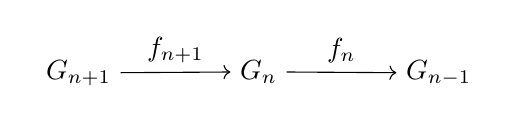
\begin{tikzpicture}
%\matrix(m)[matrix of math nodes, row sep=3em, column sep=3em, text height=1.5ex, text depth=0.25ex]
\matrix(m)[matrix of math nodes, row sep=4em, column sep=4em]
{
	G_{n+1}   &  G_n & G_{n-1} \\
};
%\path[->,font=\scriptsize]
\path[->]
(m-1-1) edge node[auto]{$f_{n+1}$} (m-1-2)
(m-1-2) edge node[auto]{$f_n$} (m-1-3);
\end{tikzpicture} 
\end{equation}
\end{definition}

	
\begin{theorem}
	\begin{enumerate}
		\item \[
		\begin{tikzpicture}
		%\matrix(m)[matrix of math nodes, row sep=3em, column sep=3em, text height=1.5ex, text depth=0.25ex]
		\matrix(m)[matrix of math nodes, row sep=4em, column sep=4em]
		{
			1   &  A & B \\
			%\path[->,font=\scriptsize]
		};
		\path[->]
		(m-1-2) edge node[auto]{$f$} (m-1-3);
		\end{tikzpicture} 
		\]
		\item \[
		\begin{tikzpicture}
		%\matrix(m)[matrix of math nodes, row sep=3em, column sep=3em, text height=1.5ex, text depth=0.25ex]
		\matrix(m)[matrix of math nodes, row sep=4em, column sep=4em]
		{
			B   &  C & 1 \\
		};
		%\path[->,font=\scriptsize]
		\path[->]
		(m-1-1) edge node[auto]{$g$} (m-1-2);
		\end{tikzpicture} 
		\]
		\item \[
		\begin{tikzpicture}
		%\matrix(m)[matrix of math nodes, row sep=3em, column sep=3em, text height=1.5ex, text depth=0.25ex]
		\matrix(m)[matrix of math nodes, row sep=4em, column sep=4em]
		{
			1 & A   &  B & 1 \\
		};
		%\path[->,font=\scriptsize]
		\path[->]
		(m-1-2) edge node[auto]{$h$} (m-1-3);
		\end{tikzpicture} 
		\]
		
	\end{enumerate}
\end{theorem}

\begin{proof}
	\begin{enumerate}
		\item $\text{im}(1\to A)=1$, since $1\to A$ is a group homomorphism $((1\to A)(1) = 1_A)$.  \\
		if $1\to A \xmapsto[]{f} B$ exact, $\text{ker}f = \text{im}(1\to A)=1$, so if $f(x)=1$, $x=1$, $f$ injective.  \\
		If $f$ injective, $\text{ker}f=1$.  $1=\text{im}(1\to A)$.  $1\to A \xmapsto{f}B$, exact.  
		\item $\text{ker}(C\to 1) = C$, by def. of $C\to 1$ \\
		if $B \xmapsto{g} C \to 1$ exact, $\text{im}g = g(B) = \text{ker}(C\to 1)= C$.  $g(B) = C$ implies $g$ surjective.  \\
		If $g$ surjective, $g(B) = C =\text{ker}(C\to 1)$.  $B\xmapsto{g} C \to 1$ exact.  
		\item From (i), $1\to A \xmapsto{h}B$ exact iff $h$ injective.  
		From (ii), $A\xmapsto{h}B \to 1$, exact iff $h$ surjective.  \\
		$h$ isomorphism.  
	\end{enumerate}
\end{proof}








% 20170925 END





\subsection{1st, 2nd, 3rd Isomorphism Theorems}

\begin{theorem}[1st Isomorphism Theorem (Modules) Thm. 7.8 of Rotman (2010) \cite{JRotman2010}]
If $f:M\to N$ is $R$-map of modules, then $\exists \, R$-isomorphism s.t. 
\begin{equation}
	\begin{aligned}
	& \varphi : M /\text{ker}f \to \text{im}f \\ 
	& \varphi: m + \text{ker}f \mapsto f(m)
\end{aligned} \qquad \qquad \, 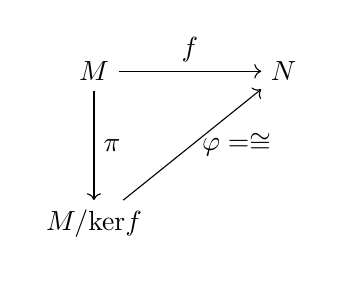
\begin{tikzpicture}
%\matrix(m)[matrix of math nodes, row sep=3em, column sep=3em, text height=1.5ex, text depth=0.25ex]
\matrix(m)[matrix of math nodes, row sep=4em, column sep=4em]
{
M   &  N \\
M/\text{ker}f  &  \\};
%\path[->,font=\scriptsize]
\path[->]
(m-1-1) edge node[auto]{$f$} (m-1-2)
edge node[auto]{$\pi$} (m-2-1) 
(m-2-1) edge node[right]{$\varphi = \cong$} (m-1-2);
\end{tikzpicture} 
\end{equation}
%Essentially, 
%\begin{equation}

%\end{equation}
\end{theorem}

\begin{proof}
	View $M,N$ as abelian groups.  

Recall natural map $ \begin{aligned} & \quad \\ 
	& \pi : M \to M/N \\
& m\mapsto m + N \end{aligned}$  

Define $\varphi$ s.t. $\varphi \pi = f$.  

($\varphi$ well-defined).  Let $m+\text{ker}f = m' + \text{ker}f$, $m,m' \in M$, then $\exists \,  n \in \text{ker}f$ s.t. $m=m'+n$.  
\[
\varphi(m+\text{ker}f) = \varphi\pi (m) = f(m) = f(m' +n ) = f(m') + f(n) = \varphi \pi(m') + 0 = \varphi(m' + \text{ker}f )
\]
$\Longrightarrow \varphi $ well-defined.  

($\varphi$ surjective).  Clearly, $\text{im}\varphi \subseteq  \text{im} f$.   \\
Let $y\in \text{im}f$.  So $\exists \,  m \in M$ s.t. $y=f(m)$.  $f(m) = \varphi \pi (m) = \varphi(m+\text{ker}f) = y$.  So $y\in \text{im}\varphi$.  $\text{im}f\subseteq \text{im}\varphi$.  \\
$\Longrightarrow \varphi $ surjective.  

($\varphi$ injective)  If $\varphi(a+\text{ker}f) = \varphi(b+\text{ker}f)$, then 
\[
\begin{gathered}
\varphi\pi(a) = \varphi\pi(b) \text{ or } f(a) = f(b) \text{ or } 0 = f(a) -f(b) = f(a-b) \text{ so } a-b \in \text{ker}f
	(a-b) + \text{ker}f = \text{ker}f \text{ so } a + \text{ker}f = b +\text{ker}f 
\end{gathered}
\]
$\varphi$ isomorphism.  

$\varphi$ $R$-map.  $\varphi(r(m+N)) = \varphi(rm+N) = f(rm)$.    \\
Since $f$ $R$-map, $f(rm) = rf(m) = r\varphi(m+N)$.  $\varphi$ is $R$-map indeed.  


\end{proof}


\begin{theorem}[2nd Isomorphism Theorem (Modules) Thm. 7.9 of Rotman (2011) \cite{JRotman2010}]
If $S,T$ are submodules of module $M$, i.e. $S,T \in M$, then $\exists \, $ $R-$isomorphism  
\begin{equation}
\begin{gathered}
	S/(S\cap T) \to (S+T)/T
\end{gathered} \qquad \, 
\qquad \qquad \, 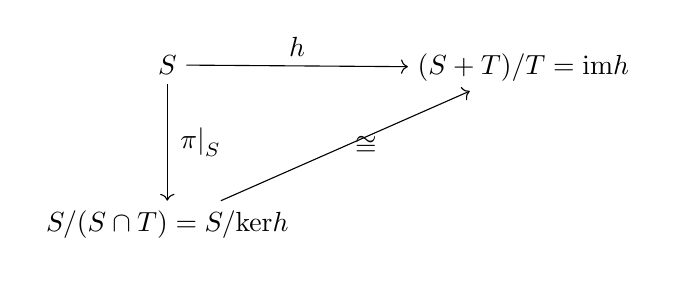
\begin{tikzpicture}
\matrix(m)[matrix of math nodes, row sep=4em, column sep=4em]
{
S   &  (S+T)/T = \text{im}h \\
S/(S\cap T) = S/\text{ker}h  &  \\};
\path[->]
(m-1-1) edge node[auto]{$h$} (m-1-2)
edge node[auto]{$\left. \pi \right|_S$} (m-2-1) 
(m-2-1) edge node[right]{$ \cong$} (m-1-2);
\end{tikzpicture} 
\end{equation}
\end{theorem}

\begin{proof}
Let natural map $\pi : M \to M/T$.   \\
\phantom{Let} So $\text{ker}\pi = T$.  

Define $h:= \left. \pi \right|_S$, so $h: S\to M/T$, so $\text{ker}h = S\cap T$, 
\[
(S+T)/T = \lbrace (s+t) + T | a\in S+T, s\in S, t\in T \rbrace
\]
i.e. $(S+T)/T$ consists of all those cosets in $M/T$ having a representation in $S$.  

By 1st. isomorphism theorem, 
\[
S/S\cap T \xrightarrow{ \cong} (S+T)/T
\]

\end{proof}  % END of pf. of 2nd Isomorphism Theorem (Modules) Thm. 7.9 of Rotman (2011)

\begin{theorem}[3rd Isomorphism Theorem (Modules) Thm. 7.10 of Rotman (2011) \cite{JRotman2010}]
If $T\subseteq S \subseteq M$ is a tower of submodules, then $\exists \, $ $R$-isomorphism
\begin{equation}
\begin{gathered}
	(M/T)/(S/T) \to M/S
\end{gathered} \qquad \,  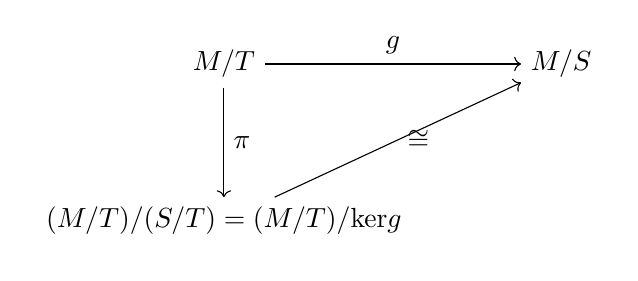
\begin{tikzpicture}
\matrix(m)[matrix of math nodes, row sep=4em, column sep=4em]
{
M/T   &  M/S\\
(M/T)/(S/ T) = (M/T)/\text{ker}g  &  \\};
\path[->]
(m-1-1) edge node[auto]{$g$} (m-1-2)
edge node[auto]{$ \pi $} (m-2-1) 
(m-2-1) edge node[right]{$ \cong$} (m-1-2);
\end{tikzpicture} 
\end{equation}
\end{theorem}

\begin{proof}
	Define $g:M/T \to M/S$ to be \textbf{coset enlargement}, i.e. 
\begin{equation}
	g:M +T \mapsto m+S
\end{equation}
$g$ well-defined: if $m+T = m'+T$, then $m-m' \in T\subseteq S$, and $m+S = m'+S \Longrightarrow g(m+T) = g(m'+T)$

$\text{ker}g = S/T$ since 
\[
\begin{aligned}
	& g(s+T) = s+S = S  \qquad \, (S/T \subseteq \text{ker}g)   \\
	& g(m+T) = m + S = 0 = S = s + S, \text{ so } m=s \Longrightarrow \text{ker}g \subseteq S/T
\end{aligned}
\]
$\text{im}g = M/S $ since 
\[
\begin{aligned}
	& g(m+T) = m+S \Longrightarrow \text{ im}g \subseteq M/S \\ 
 	& m+S = g(m+T)
\end{aligned}
\]
Then by 1st isomorphism, and commutative diagram, done.  
\end{proof} % END of pf. of 3rd Isomorphism Theorem (Modules) Thm. 7.10 of Rotman (2011) 

\section{Rings} 

\begin{definition}[division ring]
	ring $R$ with identity $1$, where $1\neq 0$ is a \textbf{division ring} (or skew field) if $\forall \, a \in R$, $a\neq 0$, $\exists \, $ multiplicative inverse $1/a$, i.e. $\exists \, b\in R$ s.t. $ab=ba = 1$
\end{definition}

e.g. 
\begin{enumerate}
	\item rational numbers $\mathbb{Q}$ \\
	real numbers $\mathbb{R}$ \\
	complex numbers $\mathbb{C}$ \\ 
	are commutative rings with identity (in fact, they're fields) \\
	Ring axioms for each follow ultimately from ring axioms for $\mathbb{Z}$ \\
	(verified when $\mathbb{Z}$ constructed from $\mathbb{Z}$ (Sec. 7.5)), $\mathbb{C}$ from $\mathbb{R}$ (Example 1, Sec. 13.1). \\
	Construction of $\mathbb{R}$ from $\mathbb{Z}$ carried out in basic analysis texts
	\item \textbf{quotient group} $\mathbb{Z}/n\mathbb{Z}$ is a commutative ring with identity (element 1) under operations of addition and multiplication of residue classes (frequently referred to as "modular arithmetic").  \\
	We saw additive abelian groups axioms followed from general principles of theory of quotient groups ($\mathbb{Z}/n\mathbb{Z}$) was prototypical quotient group. cf. Example 4, pp. 224, Dummit and Foote (2014)\cite{DuFo2003}
	\item \textbf{the (real) Hamiltonian Quaternions}.  
	\begin{definition}[(real) Hamiltonian Quaternions]
		Let $\mathbb{H} = \lbrace a+ bi + cj + dk | a,b,c,d \in \mathbb{R} \rbrace$ s.t. 
		"componentwise" addition is defined as 
		\begin{equation}
		(a+bi + cj+dk) + (a' + b'i + c'j + d'k) = (a+a') + (b+b')i + (c+c')j + (d+d')k
		\end{equation} and multiplication defined by expanding using distributive laws 
		\[
		(a+bi + cj +dk)(a' + b'i + c'j +d' k)
		\]
		using 
		\begin{equation}
		\begin{aligned}
		& i^2 = j^2 =k^2 = -1 \\
		& ij = -ji = k \\
		& jk = -kj = i \\
		& ki = -ik = j
		\end{aligned}
		\end{equation}
	\end{definition}
Working out the multiplication
\[
\begin{gathered}
(a+bi + cj + dk)(a'+b'i + c'j + d'k) =  \\
= \begin{aligned}
& aa' + ab' i + ac'j + ad'k + ba' i - bb' + bc' k -bd' j + \\
& ca'j - cb' k - cc' + cd' i + da' k + db' j - dc' i -dd' = \\
\end{aligned} \\
= aa' - bb' -cc' -dd' + (ab' + ba' + cd' -dc')i + (ac' - bd' + ca' +db')j + (ad' + bc' - cb' + da')k 
\end{gathered}
\]
Hamiltonian Quaternions are noncommutative ring with identity ($1= 1 + 0i + 0j + 0k$). 

Similarly define \emph{rational} Hamiltonian Quaternions ring by taking $a,b,c,d\in \mathbb{Q}$.  

real and rational Hamiltonian Quaternions both are divison rings, where inverse of nonzero element defined as 


\begin{equation}
(a+bi +cj + dk)^{-1} = \frac{ a-bi -cj -dk}{ a^2 + b^2 + c^2 + d^2 }
\end{equation} cf. Example 5, pp. 224, Dummit and Foote (2014)\cite{DuFo2003}

\item \textbf{rings of functions} (important class) \\
Let $X$ be any nonempty set. \\
Let $A$ be any ring. 

\begin{definition}[function ring]
	collection $R= \lbrace f:X\to A \rbrace$ is a ring under pointwise addition and multiplication of functions s.t. 
	\begin{equation}
	\begin{aligned}
	(f+g)(x) & = f(x) + g(x) \\
	(fg)(x) & = f(x)g(x)
	\end{aligned}
	\end{equation}
\end{definition}
	
cf. Example 6, pp. 225, Dummit and Foote (2014)\cite{DuFo2003}
	
\end{enumerate}

\section{Commutative Rings}

cf. Ch. 3 "Commutative Rings I" of Rotman (2010) \cite{JRotman2010}


\begin{definition} commutative ring $R$ is a set with 2 binary operations, addition and multiplication, s.t.
	\begin{enumerate}
		\item[(i)] $R$ abelian group under addition 
		\item[(ii)] (commutativity) $ab=ba$ \quad $\forall \, a,b \in R$  (this isn't there for noncommutativity)
		\item[(iii)] (associativity) $a(bc) = (ab)c$ \quad \, $\forall \, a,b,c\in R$
		\item[(iv)] $\exists \, 1 \in R$ s.t. $1a = a$ \, $\forall \, a  \in R$ \quad \, (many names used: one, unit, identity)
		\item[(v)] (distributivity) $a(b+c) = ab+ac$ \quad \, $a,b,c \in R$ (this splits up into 2 distributivity laws for noncommutativity)
	\end{enumerate}
\end{definition}

To reiterate, abelian group under addition $R$ (is defined as)
\begin{enumerate}
	\item associative $\forall \, x , y ,z \in R$, $x + (y+z) = (x+y)+z$ 
	\item $\exists \, 0 \in R$, $0+x = x + 0$, \, $\forall \, x \in R$ 
	\item $\forall \, x \in R$, $\exists \, (-x) \in R$ s.t. $x+(-x) = 0 = (-x) + x$
\end{enumerate}
abelian, if commutativity: $x+y=y+x$.  

\subsection{Linear Algebra; Linear Algebra with commutative rings as fields}

\subsubsection{Linear Algebra}

\begin{definition}[subspace]
	If $V$ vector space over field $k$, \\
	then \textbf{subspace} of $V$ is subset $U$ of $V$ s.t. 
	\begin{enumerate}
		\item $0\in U$
		\item $u,u' \in U$ imply $u+u' \in U$ 
		\item $u\in U$, and $a\in k$ imply $au \in U$
	\end{enumerate}
	\textbf{proper subspace} of $V \equiv U \subsetneq V$ is subspace $U \subseteq V$ with $U \neq V$.
\end{definition}
$U =V$, $U = \lbrace 0 \rbrace$ are always subspaces of a vector space $V$. 

\textbf{Examples} (Example 3.70 Rotman (2010) \cite{JRotman2010}) 
\begin{enumerate}
	\item[(ii)] If $V=(a_1, \dots a_n)$, $v\neq 0$, $v\in \mathbb{R}^n$, \\
	line through origin $l = \lbrace av | a \in \mathbb{R} \rbrace$ is a subspace of $\mathbb{R}^n$. \\
	plane through origin $=\lbrace av_1 + bv_2 | v_1 , v_2 \text{ fixed pair of noncollinear vectors, } a,b \in \mathbb{R} \rbrace$ are subspaces of $\mathbb{R}^n$
	\item[(iii)] If $m\leq n$, $\mathbb{R}^m$ regarded as set of all vectors in $\mathbb{R}^n$ s.t. last $n-m$ coordinates are $0$, then $\mathbb{R}^m$ subspace of $\mathbb{R}^n$.
	e.g. $\mathbb{R}^2 = \lbrace (x,y,0) \in \mathbb{R}^3 \rbrace \subsetneq \mathbb{R}^3$
	\item[(iv)] If $k$ field, \textbf{homogeneous linear system over $k$ } of $m$ equations in $n$ unknowns is a set of equations
	\[
	\begin{aligned}
	a_{11} x_1 + \dots + a_{1n} x_n = 0 & \\
	a_{21} x_1 + \dots + a_{2n} x_n = 0 & \\
	\vdots \vdots & \\
		a_{m1} x_1 + \dots + a_{mn} x_n = 0 & 
	\end{aligned}
	\] 
	where $a_{ji} \in k$.
	
	\textbf{solution} of this system is vector $(c_1 \dots c_n) \in k^n$ s.t. $\sum_i a_{ji} c_i  =0$, $\forall \, j$. \\
	solution $(c_1 \dots c_n)$ \textbf{nontrivial} if $\exists$ some $c_i \neq 0$. \\
	\textbf{solution space} (or null space) of system $=$ set of all solutions. \\
	solution space also a subspace of $k^n$
\end{enumerate}

e.g. $k = \mathbb{I}_p$, 
\[
\begin{aligned}
& 3x - 2y + z \equiv 1 \bmod{7} \\
& x + y -2 z \equiv 0 \bmod{7} \\
& -x + 2y + z \equiv 4 \bmod{7}
\end{aligned}
\]
\begin{definition}[list]
	list $:=$ vector space $V$ is ordered set $v_1 \dots v_n$ of vectors in $V$, i.e. 
	$\exists \, $ some $n\geq 1$, $\exists \, $ some function $\varphi$ 
	\[
	\varphi : \lbrace 1,2\dots n \rbrace \to V
	\]
	with $\varphi(i) = v_i \quad \, \forall \, i$
\end{definition}

Thus, $X = \text{im}\varphi$.

$X$ ordered, $\varphi$ need not be injective. 

\begin{definition}[k-linear combination]
	$k$-linear combination of list $v_1\dots v_n$ in $V$, $V\equiv $ vector space over field $k$, is vector $v$ of form 
	\[
	v = a_1 v_1 + \dots + a_n v_n  = \sum_{i=1} a_i v_i \quad \, \forall \, a_i \in k, \, \quad \, \forall \, i
	\]
\end{definition}

\begin{definition}[list]
	If list $X = v_1 \dots v_m$ in vector space $V$, then \\
	\textbf{subspace spanned by } $X$, $\langle v_1 \dots v_m \rangle := $ set of all $k$-linear combinations of $v_1 \dots v_m$.  Also, say $v_1 \dots v_m $ spans $\langle v_1 \dots v_m\rangle$. 
\end{definition}

\begin{lemma}[$\langle v_1 \dots v_m \rangle$ is smallest subspace of $V$ containing $v_1\dots v_m$]\label{Lemma:smallest_subspace}
\begin{enumerate}
	\item[(i)] Every intersection of subspaces of $V$ is itself a subspace.
	\item[(ii)] If $X= v_1 \dots v_m$ list in $V$, then intersection of all subspaces of $V$ containing $X$ is $\langle v_1 \dots v_m \rangle$, subspace spanned by $v_1\dots v_m$, so $\langle v_1 \dots v_m \rangle$ is smallest subspace of $V$ containing $X$. 
\end{enumerate}
\end{lemma}
cf. (Lemma 3.71 Rotman (2010) \cite{JRotman2010}) 

\begin{proof}
\begin{enumerate}
	\item[(i)] Consider $\bigcap_{\alpha \in I} V_{\alpha}$, $\forall \, \alpha \in I$, $V_{\alpha} $ subspace of $V$
	\begin{enumerate}
		\item[(i)] $0\in V_{\alpha}$, $\forall \, \alpha \in I$, so $0\in \bigcap_{\alpha \in I} V_{\alpha}$,
		\item[(ii)] Let $u,u' \in \bigcap_{\alpha \in I} V_{\alpha}$. Then $u,u' \in V_{\alpha}$, $\forall \, \alpha \in I$. Consider $\beta \in I$. $u, u' \in V_{\beta}$, so $u+u' \in V_{\beta}$.  Without loss of generality, $u + u' \in V_{\alpha}$, $\forall \, \alpha \in I$.  Then $u+u' \in \bigcap_{\alpha \in I} V_{\alpha}$
		\item[(iii)] Let $u\in \bigcap_{\alpha \in I} V_{\alpha}$.  Consider $\alpha \in k$. Since $u\in V_{\alpha}$, $\forall \, \alpha \in I$, $au\in V_{\alpha}$, $\forall \, \alpha \in I$.  \\
		Then $au \in \bigcap_{\alpha \in I} V_{\alpha}$
	\end{enumerate}
\item[(ii)] Let $X = \lbrace v_1 \dots v_m \rbrace$, let $\mathcal{S} \equiv $ family of all subspaces of $V$ containing $X$. 

$\bigcap_{S \in \mathcal{S}} S \subseteq \langle v_1 \dots v_m \rangle$ because $\langle v_1 \dots v_m \rangle \in \mathcal{S}$, since, \\
\qquad \, $\langle v_1 \dots v_m \rangle$ is \emph{a} subspace of $V$ containing $X$. 

If $S\in \mathcal{S}$, then $S\ni v_1 \dots v_m$.  As shown above, $\forall \, v\in \langle v_1 \dots v_m \rangle$, $v\in S$, and thus $v\in \bigcap_{S\in \mathcal{S}} S$. $\langle v_1 \dots v_m \rangle \subseteq \bigcap_{S\in \mathcal{S}} S$.  
\end{enumerate}
	\end{proof}

Were all terminology in algebra consistent, \\
$\langle v_1 \dots v_m \rangle \equiv $ subspace \emph{generated} by $X$.  

Reason for different terms is that group theory, rings, vector spaces developed independently of each other.

\textbf{Example 3.72 of Rotman (2010) \cite{JRotman2010}}
\begin{enumerate}
	\item[(i)]
	\item[(ii)]
	\item[(iii)] \textbf{polynomial vector space; polynomials as a vector space}.  \\
	Vector space need not be spanned by finite list. \\
	e.g. $V=k[x]$, \\
	Suppose $X= f_1(x) \dots f_m(x)$ finite list in $V$. \\
	If $d= $ largest degree of any of $f_i(x)$, \\
	then every (nonzero) $k$-linear combination of $f_1(x), \dots f_m(x)$ has degree at most $d$. \\
	Thus $x^{d+1} \notin \langle f_1(x) \dots f_m(x) \rangle$, so $X$ doesn't span $k[x]$
\end{enumerate}

\begin{definition}[finite-dimensional vector space; infinite-dimensional vector space]
	Vector space $V$ is \textbf{finite-dimensional} if it's spanned by a finite list; otherwise $V$ is \textbf{infinite-dimensional}.
\end{definition}

\begin{proposition}[linear dependent span properties]
If vector space $V$, list $X=v_! \dots v_m$ spanning $V$, following are equivalent:
	\begin{enumerate}
		\item[(i)] $X$ isn't shortest spanning list 
		\item[(ii)] some $v_i$ is in subspace spanned by others, i.e. $v_i \in \langle v_i \dots \widehat{v}_i \dots v_m \rangle$, 
		\item[(iii)]		$\exists \, a_1 \dots a_m$ not all $0$ s.t. $\sum_{l=1}^m a_l v_l = 0$
	\end{enumerate}
\end{proposition}

\begin{proof}
(i) $\Longrightarrow$ (ii). If $X$ isn't hosrtest spanning list, then 1 of vectors in $X$ can be thrown out, and shorter list still spans, i.e. cf. Lemma \ref{Lemma:smallest_subspace}(Lemma 3.71, Rotman (2010) \cite{JRotman2010}); let $\mathcal{S} \equiv $ family of all subspaces of $V$ containing $X$. 

EY: 20180610 
Let $\bigcap_{S\in \mathcal{S}} S$. $\bigcap_{S \in \mathcal{S}} S \neq \langle v_1 \dots v_m \rangle$, $\bigcap_{S \in \mathcal{S}} S \subset \langle v_1 \dots v_m \rangle$ \\
$\exists \, v \in \langle v_1 \dots v_m \rangle$, say$v= \sum_{i=1}^m a_i v_i$ s.t. $\exists \, S \in \mathcal{S}$, s.t. $v\notin S$.  

(ii) $\Longrightarrow$ (iii) If $v_i = \sum_{j\neq i} c_j v_j$, define $a_i  = -1 \neq 0$, $a_j = c_j$, $\forall \, j \neq i$.  Then $\sum_{l=1}^m a_l v_l = -v_i + \sum_{j\neq i } c_j v_j = 0$

(iii) $\Longrightarrow$ (i) Suppose for $i \in 1 \dots m$, $a_i \neq 0$.  $v_i = -\sum_{j\neq i} \frac{a_j}{a_i} v_j$.  $\langle v_1 \dots \widehat{v}_i \dots v_m\rangle$ still spans $V$ (i.e. deleting $v_i$ gives a shorter list, which still spans).  

For instance, if $v\in \langle v_1 \dots v_m \rangle$, $v= \sum_{l=1}$%m c_l v_l = \sum_{j\neq i} c_j v_j + c_i \left( - \sum_{j\neq i} \frac{a_j}{a_i} v_j \right) = \sum_{j\neq i } \left( c_j - \frac{ c_i a_j}{a_i} \right) v_j$ so $\langle v_1\dots v_m \rangle$ wasn't shortest spanning list.





	\end{proof}

\exercisehead{3.67} Suppose $\text{dim}V >1$. Then $\exists \, $ at least 2 elements in a basis of $V$, say $e_1$, $e_2$. (Thm. 3.78 of Rotman (2010) \cite{JRotman2010}, "Every finite-dim. vector space $V$ has a basis; Def. of $\text{dim}$, "number of elements in a basis of $V$").   

Consider subspaces $\langle e_1 \rangle$, $\langle e_2 \rangle$, subspaces spanned by $e_1,e_2$, respectively. Whether $V= \langle e_1, e_2 \rangle$ or $V= \langle e_1, e_2\rangle$, $\langle e_1 \rangle , \langle e_2 \rangle \neq \lbrace 0 \rbrace$ nor $V$. Contradiction of hypothesis.  

Thus, "If only subspaces of a vector space $V$ are $\lbrace 0 \rbrace$ and $V$ itself, $\text{dim}(V) \leq 1$."



\begin{proposition}[Matrix representation of linear transformation; 3.94 of Rotman (2010) \cite{JRotman2010}]\label{Prop:MatRepofLinearTransform}
	If linear transformation $T: k^n \to k^m$, then $\exists \,  A \in \text{Mat}_k(m,n)$ s.t. 
	\[
	T(y) = Ay, \qquad \  \forall \, y \in k^n
	\]
\end{proposition}

\begin{proof}
	Let $\begin{aligned} & (e_1\dots e_n) & \text{standard basis of $k^n$ }   \\
	& (e_1' \dots e_m') & \text{standard basis of $k^m$ }  \end{aligned}$

Define $A=[a_{ij}]$, s.t. $T(e_j) = A_{*j} = A_{ij} e_i'$ ($j$th column), 

If $\begin{aligned} 
& S:k^n \to k^m \\ 
& S(y) = A(y) \end{aligned}$, then 
\[
T(e_j) = a_{ij}e_i' = Ae_j
\]
and so $\forall \, y = y_je_j \in k^n$, 
\[
T(y) = T(y_je_j) = y_j T(e_j) = y_j A_{ij}e'_i = Ay
\]


	\end{proof}


\section{R-modules}

cf. Sec. 7.1 Modules of Rotman (2010) \cite{JRotman2010}

\begin{definition}[$R$-module]
	$R$-module is (additive) abelian group $M$, \\
	equipped with scalar multiplication $\begin{aligned} & \quad \\
	& R \times M \to M \\
	& (r,m) \mapsto rm \end{aligned}$ 
	
	s.t. $\forall \, m,m' \in M$, $\forall \, r,r',1 \in R$
	\begin{enumerate}
		\item[(i)] $r(m+m')=rm+rm'$
		\item[(ii)] $(r+r')m = rm+r'm$
		\item[(iii)] $(rr')m = r(r'm)$
		\item[(iv)] $1m = m$
	\end{enumerate}
\end{definition}

Example 7.1 \begin{enumerate}
	\item[(i)] $\forall \, $ \emph{vector space} over field $k$ is a $k$-module.  (by inspection of the axioms for a vector space, associativity, distributivity!)
	\item[(ii)] $\forall \, $ abelian group is a $\mathbb{Z}$-module, by laws of exponents (Prop. 2.23)
	
	Indeed, for
	\[
	\begin{aligned}
	\mathbb{Z} \times M & \to M \\ 
	(r,m) & \mapsto rm \equiv m^r 
	\end{aligned}
	\]
	and so
	\[
	r(m\cdot m') \equiv (m\cdot m')^r = m^r (m')^r = rm + rm' 
	\]
	(since $M$ abelian)
	\item[(iii)] For commutative ring, scalar multiplication, defined to be given multiplication of elements of $R$
	\[
	\begin{aligned}
	R\times R & \to R \\
	(a,b) & \mapsto ab 
	\end{aligned}
	\]
	For reference, recall some of the properties of a commutative ring:
	\[
	\begin{aligned}
	& ab = ba \\ 
	& a(bc) = (ab)c \\ 
	& 1a = a \\ 
	& a(b+c) = ab + ac
	\end{aligned}
	\]
	
	$\forall \, $ ideal $I$ in $R$ is an $R$-module, \\
	for if $\begin{aligned} & \quad \\
	& i \in I \\
	& r\in R \end{aligned}$ , then $ri \in I$.
	
	$0\in I$ \\
	$\forall \, a,b \in I, \, a+b \in I$
	
	
	If $a\in I$, $r\in R$, then $ra \in I$.
	
	
	\item[(iv)]
	\item[(v)] Let linear $T:V \to V$, $V$ finite-dim. vector space over field $k$.  
	
	Recall $k[x] \equiv $ set of polynomials with coefficients in $k$.  
	
	Define $\begin{aligned} & \quad \\
	& k[x] \times V \to V \\
	& f(x)v =\left(\sum_{i=0}^m c_i x^i\right)v =\sum_{i=0}^m c_iT^i(v) \end{aligned}$ \quad \, $\forall \, f(x) = \sum_{i=0}^m c_ix^i \in k[x]$
	
	$\Longrightarrow $ denote $k[x]$-module $V^T$.  
	
	Special case: Let $A \in \text{Mat}_k(n,n)$, let linear $\begin{aligned} & \quad \\
	& T :k^n \to k^n \\
	& T(w) = Aw \end{aligned}$.  
	
	vector space $k^n$ is $k[x]$-module if we define scalar multiplication 
	\[
	\begin{aligned} & \quad \\
	& k[x] \times k^n \to k^n \\
	& f(x)w = \left( \sum_{i=0}^m c_ix^i \right)w = \sum_{i=0}^m c_i A^i w \end{aligned}
	\] 
	\quad \, $\forall \, f(x) = \sum_{i=0}^m c_ix^i \in k[x]$
	
	In $(k^n)^T$, $xw = T(w)$ \\
	In $(k^n)^A$, $xw = Ax $ \\
	$T(w) = Ax$ and so $(k^n)^T = (k^n)^A$  (EY : 20151015 because of induction?)
\end{enumerate}


\begin{definition}[R-homomorphism (or R-map)]
If ring $R$, $R$-modules $M,N$, then \\
function $f: M\to N$, \\
if $\forall \, m, m' \in M$, $\forall \, r\in R$, 
\[
\begin{gathered}
	f(m+m') = f(m) + f(m') \\ 
f(rm) = rf(m)
\end{gathered}
\]
\end{definition}

Example 7.2. of Rotman (2011) on pp. 425 \cite{JRotman2010}] 

\begin{enumerate}
	\item[(i)] If $R$ field, then $R$-modules are vector spaces and $R$-maps are linear transformations.  Isomorphisms are then nonsingular linear transformations.  
	\item[(ii)] 
	\item[(iii)]
	\item[(iv)]
	\item[(v)] Let linear $T:V \to V$, let $v_1 \dots v_n$ be basis of $V$, let $A$ be matrix of $T$ relative to this basis.  
	
	Let $e_1 \dots e_n$ be standard basis of $k^n$.  \\
	Define $\begin{aligned} & \quad \\
	& \varphi : V \to k^n \\
	& \varphi(v_i) = e_i \end{aligned}$
	
	\[
	\begin{aligned}
	& \varphi(xv_i) = \varphi(T(v_i)) = \varphi(v_j a_{ji} ) = a_{ji} \varphi(v_j) = a_{ji}e_j \\
	& x\varphi(v_i) = A\varphi(v_i) = Ae_i
	\end{aligned}
	\]
	$\Longrightarrow \varphi(xv) = x\varphi(v) \quad \, \forall \, v \in V$
	
	By induction on $\text{deg}(f)$, $\varphi(f(x)v) = f(x) \varphi(v)$ \quad \, $\forall \, f(x) \in k[x]$ \quad \, $\forall \, v \in V$ 
	
	$\Longrightarrow \varphi$ is $k[x]$-map \\
	$\Longrightarrow \varphi$ is $k[x]$-isomorphism of $V^T$ and $(k^n)^A$.  
	
\end{enumerate}


\begin{proposition}[7.3 of Rotman (2011) \cite{JRotman2010}]\label{Prop:kxmoduleisomorphism}
	Let vector space over field $k$, $V$, let linear $T,S : V \to V$ \\
	Then $k[x]$-modules $V^T, V^S$ are $k[x]$-isomorphic iff $\exists \, $ vector space isomorphism $\varphi : V \to V$ s.t. $S = \varphi T \varphi^{-1}$.  
\end{proposition}

\begin{proof}
	If $\varphi:V^T \to V^S$is a $k[x]$-isomorphism, 
	\[
	\varphi(f(x)v) = f(x)\varphi(v) \quad \, \forall \, v \in V , \, \forall \, f(x) \in k[x]
	\]
	if $f(x)=x$, then $\varphi(xv) = x\varphi(v)$
	\[
	\begin{aligned}
	& xv = T(v) \\ 
	& x\varphi(v) = S(\varphi(v)) \\ 
	\Longrightarrow & \varphi \circ T(v) = S \circ \varphi(v) \Longrightarrow \varphi \circ T = S \circ \varphi 
	\end{aligned}
	\]
	$\varphi$ isomorphism, so $S = \varphi \circ T \circ \varphi^{-1}$
	
	Conversely, if given isomorphism $\varphi: V \to V$ s.t. $S = \varphi T \varphi^{-1}$, then $S\varphi = \varphi T$.  
	\[
	S\varphi(v) = \varphi T(v) = \varphi(xv) = x\varphi(v)
	\]
	Then by induction, $\varphi(x^nv) = x^n\varphi(v)$ (for $S^n\varphi(v) = x^n\varphi(v) = (\varphi T \varphi^{-1})^n \varphi(v) = \varphi T^n v = \varphi(x^nv)$).  \\
	By induction on $\text{deg}(f)$, $\varphi(f(x)v) = f(x)\varphi(v)$.  
	
	
\end{proof}



\begin{corollary}[7.4 of Rotman (2011) \cite{JRotman2010}] 
	Let $k$ be a field, \\
	Let $A,B \in \text{Mat}_k(n,n)$.  \\
	Then $k[x]$-modules $(k^n)^A$, $(k^n)^B$ are $k[x]$-isomorphic.  
	
	(recall, $k[x]\equiv $ set of polynomials with coefficients in $k = \lbrace \sum_{i=0}^m c_ix^i | c_i \in k \rbrace$, and define scalar multiplication 
	\[
	\begin{aligned}
		& k[x] \times k^n \to k^n \\
		& f(x) w = \left( \sum_{i=0}^m c_i x^i \right) w = \sum_{i=0}^m c_iA^i w, \qquad \  \forall \, f(x) = \sum_{i=0}^m c_i x^i \in k[x] 
	\end{aligned}
	\]
	)
	
	iff $\exists \, $ nonsingular $P$ with 
	\[
	B=PAP^{-1}
	\]
	
	\end{corollary}

\begin{proof}
	Define 
	
	$\begin{aligned} & T:k^n \to k^n \\
	& T(y) = A(y) \end{aligned}$
where $y\in k^n $ is a column.  

By Example 7.1 (v) of Rotman (2011)  \cite{JRotman2010}, recall, 

and so for $k[x]$-module, $(k^n)^T = (k^n)^A$.  

Similarly, define 
\[
\begin{aligned} 
	& S: k^n \to k^n  \\
	& S(y) = B(y) 
	\end{aligned}
	\]
	Denote corresponding $k[x]$-module by $(k^n)^B$.  
	
	Given $(k^n)^A \cong (k^n)^B$ (isomorphic), by Prop. \ref{Prop:kxmoduleisomorphism}, \\
	$\exists \, $ isomorphism $\varphi :k^n \to k^n$ s.t. $B=\varphi A \varphi^{-1}$.  

By Prop. \ref{Prop:MatRepofLinearTransform}, i.e. Prop. 3.94 of Rotman (2011)  \cite{JRotman2010}, in that every linear transformation has a matrix representation (even in the standard "Euclidean" basis), $\exists \,  P \in \text{Mat}_{k}(n,n)$, s.t. 
\[
\varphi(y) = Py \qquad \  y\in k^n
\]
($P$ nonsingular because $\varphi$ isomorphism)

Thus, 
\[
\begin{aligned}
& B\varphi(y) = \varphi A(y)  \\ 
& BPy = P(Ay) \qquad \  \forall \, y \in k^n  \\
\Longrightarrow & PA = BP \text{or } B= PAP^{-1}
\end{aligned}
\]

Conversely, given $B=PAP^{-1}$, $P$ nonsingular matrix,  \\
define isomorphism 
\[
\begin{aligned}
& \varphi :k^n \to k^n \\ 
& \varphi(y) = Py \qquad \  \forall \, y \in k^n
\end{aligned}
\]

By Prop. \ref{Prop:kxmoduleisomorphism}, \\
$(k^n)^B$, $(k^n)^A$ are $k[x]$-isomorphic.  \\
i.e. $\varphi : (k^n)^A \to (k^n)^B $ is a $k[x]$-module isomorphism.  


	\end{proof}

\begin{definition}[$\text{Hom}_R(M,N)$]
\begin{equation}
\text{Hom}_R(M,N) = \lbrace \text{ all $R$-homomorphisms $M\to N$ } \rbrace = \lbrace f | f:M\to N , \text{ s.t. } \forall \, m,m' \in M, \, \forall \, r \in R, \begin{aligned} & f(m+m') =f(m) + f(m') \\ & f(rm) = rf(m) \end{aligned} \rbrace
\end{equation}
If $f,g \in \text{Hom}_R(M,N)$, \\
define
\begin{equation}
\begin{aligned}
& f+g:M \to N \\
& f+g:m\mapsto f(m) + g(m)
\end{aligned}
\end{equation}
\end{definition}

\begin{proposition}[$\text{Hom}_R(M,N)$ $R$-module, 7.5 of Rotman (2011)  \cite{JRotman2010}]
	If $M,N$ $R$-modules, where $R$ commutative ring, \\
	then $\text{Hom}_R(M,N)$ $R$-module, \\
	with addition 
	\[
	\begin{aligned}
	& f+g: M\to N \qquad \  \forall \, f,g \in \text{Hom}_R(M,N) \\
	& f+g:m\mapsto f(m) + g(m)
	\end{aligned}
	\]
and scalar multiplication 
\[
rf:m \mapsto f(rm)
\]
	Moreover, distributive laws: \\
	If $p:M'\to M$, $q:N\to N'$, then 
	\[
	(f+g)p = fp+gp \text{ and } q(f+g) = qf + qg
	\]
$\forall \, f,g \in \text{Hom}_R(M,N)$	
	
	
	
\end{proposition}

\begin{proof}
	$\forall \, f,g \in \text{Hom}_R(M,N)$, $\forall \, r,r', 1 \in R$, 
	\begin{enumerate}
		\item[(i)] 
		\[
		r(f+g)(m) = (f+g)(rm) = f(rm) + g(rm) = rf(m) + rg(m) = (rf+rg)(m) 
		\]
		\item[(ii)]
		\[
		(r+r')f(m) = f((r+r')m) = f(rm+r'm) = f(rm) + f(r'm) = (rf+ r'f)(m)
		\]
		\item[(iii)]
		\[
		(rr')f(m) = f(rr'm) = rf(r'm) = f(r'rm) = f(rr'm) \Longrightarrow (rr')f = r(r'f)
		\]
		\item[(iv)]
		\[
		1f(m) = f(1m) = f(m) \Longrightarrow 1f =f
		\]
	\end{enumerate}
	\end{proof}



\begin{definition}
	if $R$-module $M$, the submodule $N$ of $M$, denoted $N\subseteq M$, is additive subgroup $N$ of $M$, \\
	closed under scalar multiplication $rn \in N$ whenever $n\in N$, $r\in R$
\end{definition}




\begin{definition}[quotient module $M/N$] \qquad \, \\ 
\textbf{quotient module} $M/N$  -

For submodule $N$ of $R$-module $M$, then, \\
remember $M$ abelian group, $N$ subgroup, \\
quotient group $M/N$ equipped with scalar multiplication 
\[
\begin{gathered}
	r(m+N) = rm+N \\ 
M/N = \lbrace m +N | m \in M \rbrace
\end{gathered}
\]
\textbf{natural map} 
\begin{equation}
\begin{aligned}
& \pi : M \to M /N \\ 
& m\mapsto m + N 
\end{aligned}
\end{equation}
easily seen to be $R$-map.  

Scalar multiplication in quotient module well-defined: \\
If $m+N=m'+N$, $m-m' \in N$, so $r(m-m') \in N$ (because $N$ submodule), so 
\[
rm - rm' \in N \text{ and } rm+ N = rm' +N
\]


\end{definition}


\begin{proposition}[7.15 of Rotman (2010) \cite{JRotman2010}]  
\begin{enumerate}
\item[(i)] $S \bigsqcup T \simeq M$ 
\item[(ii)] $\exists \, $ injective $R$-maps $\begin{aligned} & \quad \\ 
	& i : S\to M \\ 
& j :T \to M \end{aligned}$, s.t. 

\begin{equation}
\begin{gathered} 
M = \text{im}(i) + \text{im}(j)  \text{ and } \\ 
\text{im}(i) \bigcap \text{im}(j) = \lbrace 0 \rbrace  
\end{gathered}
\end{equation}
\item[(iii)] $\exists \, $ R-maps 
\[
\begin{aligned}
	& i : S\to M \\ 
	& j : T\to M 
\end{aligned}
\]
s.t. $\forall \, m \in M$, $\exists \, !$ 
\[
\begin{aligned}
	& s \in S \\ 
	& t \in T 
\end{aligned}
\] with $m=is + jt$.  
\item[(iv)] $\exists \, $ R-maps 
\[
\begin{gathered}
\begin{aligned}  & i: S\to M \\ 
& j:T \to M \end{aligned} \qquad \, \begin{aligned}
& p : M \to S \\ 
& q : M \to T \end{aligned}
\end{gathered}
\]
s.t. 
\[
\begin{gathered}
	\begin{aligned}
	& pi = 1_S \\ 
& qj = 1_T 
\end{aligned} \qquad \ , \begin{aligned}
	& pj = 0  \\
	& qi = 0 
\end{aligned} \qquad \, ip + jq = 1_M
\end{gathered}
\]
\end{enumerate}
\end{proposition}

\begin{proof}
\begin{itemize}
\item (i)$\to$ (ii)  Given $S \bigsqcup T \simeq  M$,  \\ 
 let $\varphi : S \bigsqcup T \to   M$ be this isomorphism.  

Define
\[
\begin{aligned}
	& i:= \varphi \lambda_S \qquad \, & (\lambda_S : s\mapsto (s,0)) \qquad \, & i :S \to M \\ 
	& j:= \varphi \lambda_T \qquad \, & (\lambda_T : t\mapsto (0,t)) \qquad \, & j :T \to M 
\end{aligned}
\]
$i,j$ are injections, being composites of injections.  

If $m\in M$, $\exists \, ! \, (s,t) \in S\bigsqcup T$, s.t. $\varphi(s,t)=m$.  

Then 
\[
m = \varphi(s,t) = \varphi((s,0) + (0,t)) = \varphi\lambda_S(s)  \varphi \lambda_T(t) = is + jt \in \text{im}(i) + \text{im}(j)
\]

Let $c\in \text{im}(i) + \text{im}(j)$.  Since $\begin{aligned}  & \quad \\ 
	& i : S\to M \\
& j : T \to M \end{aligned}$, $c\in M$.  

$\Longrightarrow M = \text{im}(i) + \text{im}(j)$.  



If $x\in \text{im}(i) \bigcap \text{im}(j)$, 
\[
\begin{aligned}
	& x = i(s) \text{ for some } s\in S \\ 
		& x = j(t) \text{ for some } t\in T  
\end{aligned}
\]

\[
\begin{gathered}
	is=jt = \varphi \lambda_S(s) = \varphi \lambda_T(t) = \varphi(s,0) = \varphi(0,t) 
\end{gathered}
\]
$\varphi$ isomorphism, so $\exists \, \varphi^{-1}$ $\Longrightarrow (s,0) = (0,t)$, so $s=t=0$.  $x=0$  
\item (ii)$\to $ (iii) Given $\begin{aligned} & \quad \\ & i:S\to M \\ & j:T\to M \end{aligned}$, s.t. $M= \text{im}(i) + \text{im}(j)$, so \\

$\forall \, m \in M$, $m=i(s) + j(t)$ for some $s\in S,t\in T$.  

Suppose $\begin{aligned} & \quad \\ 
	& s' \in S \\
& t' \in T \end{aligned}$, s.t. $m=i(s'_ + j(t')$.  
\[
i(s-s') = j(t-t') \in \text{im}(i) \bigcap \text{im}(j) = \lbrace 0 \rbrace
\]
So $s=s',t=t'$, since $i,j$ injective.  
\item (iii)$\to$ (iv)   

Given $\forall \, m \in M$, $\exists \, ! \, s\in S,t\in T$ s.t. 
\[
m=i(s) + j(t)
\]
Define 
\[
\begin{aligned}
	& p:M \to S \\ 
	& p(m) := s
\end{aligned} \qquad \, \begin{aligned}
	& q: M \to T \\ 
	& q(m) := t
\end{aligned}
\]
\[
\begin{aligned}
	& pi(s) = s \\ 
	& qj(t) = t 
\end{aligned} \qquad \, \begin{aligned}
& pj(t) =0  \\
& qi(s) = 0 \end{aligned} \qquad \, 
(ip+jq)(m) = ip(m) + jq(m) = i(s) + j(t) = m 
\]
\end{itemize}
\end{proof}

\section{Categories; Category Theory}  

\subsection{Categories}

cf. 7.2 Categories of Rotman (2010) \cite{JRotman2010}

\subsubsection{Russell paradox, Russell set}  

\begin{definition}[Russell set]
Russell set  - set $S$ that's not a member of itself, i.e. $S\notin R$
\end{definition}

If $R$ is family of all Russell sets,  \\
Let $X\in R$.  Then $X\notin X$.  But $X\in R$.  $X\notin R$.  \\
Let $R\notin R$.  Then $R$ in family of Russell Sets.  $R\in R$.  Contradiction.  

Then consider \emph{class} as primitive term, instead of set.  

\begin{definition}[Category]
Category $\mathcal{C}$ (Rotman's notation) $\equiv \mathbf{C}$ (my notation), consists of class $\text{obj}(\mathcal{C})$ (Rotman's notation) $\equiv \text{Obj}(\mathbf{C}) \equiv \text{Obj}\mathbf{C}$ (my notation) of objects, set of  morphisms $\text{Hom}(A,B)$ $\forall \,  (A,B)$ of ordered tuples of objects, composition 
\[
\begin{gathered} 
	\text{Hom}(A,B)\times \text{Hom}(B ,C) \to \text{Hom}(A,C) \\
(f,g)\mapsto gf \end{gathered}
\], s.t.
\begin{enumerate}
\item $\exists \, \mathbf{1}$, $\forall \, f:A\to B$, $\exists \, \begin{aligned} & \quad \\ 
1_A : A \to A \\
1_B : B \to B \end{aligned}$, s.t. $1_B \cdot f = f= f\cdot 1_A$, and 
\item associativity, $\forall \, \begin{aligned} & \quad \\
& f : A\to B \\
& g: B\to C \\
& h: C\to D \end{aligned}$, then $h\circ (g\circ f) = (h\circ g) \circ f$ 
\end{enumerate}

In summary, 
\begin{equation}
	\mathbf{C} := (\text{Obj}(\mathbf{C}), \text{Mor}\mathbf{C}, \circ, \mathbf{1}) \equiv (\text{Obj}\mathbf{C}, \text{Mor}\mathbf{C}, \circ_{\mathbf{C}}, \mathbf{1}_{\mathbf{C}})
\end{equation}
s.t. 
\[
\text{Mor}\mathbf{C} = \bigcup_{A,B \in \text{Obj}\mathbf{C}} \text{Hom}(A,B)
\]
\end{definition}

Examples (7.25 of Rotman (2010)\cite{JRotman2010}): 
\begin{enumerate}
\item[(i)] $\mathbf{C} = \mathbf{\text{Sets}}$  
\item[(ii)] $\mathbf{C} = \mathbf{\text{Groups}} = \mathbf{\text{Grps}}$ 
\item[(iii)]  $\mathbf{C} = \mathbf{\text{CommRings}}$
\item[(iv)]  $\mathbf{C} = {}_R\textbf{Mod}$, if $R=\mathbb{Z}$, ${}_{\mathbb{Z}}\textbf{Mod} = \textbf{Ab}$, i.e. $\mathbb{Z}-$modules are just abelian groups.   
\item[(v)] $\mathbf{C} =\textbf{PO}(X)$, If partially ordered set $X$, regard $X$ as category, s.t. $\textbf{Obj}, \textbf{PO}(X) = \lbrace x | x\in X\rbrace$, $\forall \, \text{Hom}(x,y) \in \textbf{Mor}_{\textbf{PO}}(X)$, $\text{Hom}(x,y) = \begin{cases} \emptyset & \text{ if } x \npreceq y \\  \kappa_y^x & \text{ if } x \preceq y   \end{cases}$ where $\kappa_y^x \equiv $ unique element in $\text{Hom}$ set when $x \preceq y$) s.t. 
\[
\kappa_z^y \kappa_y^x  =\kappa_z^x
\]
Also, notice that 
\[
1_x = \kappa_x^x
\]
\end{enumerate}

\begin{definition}[isormorphisms or equivalences]
$f:A\to B$, $f\in \text{Hom}(A,B)$, if $\exists \, $ \textbf{inverse} $g:B\to A$, $g\in \text{Hom}(B,A)$, s.t. 
\[
\begin{aligned}
& gf = 1_A \\ 
& fg = 1_B
\end{aligned}
\]
and if $\mathbf{C} = \textbf{Top}$, equivalences (isomorphisms) are homeomorphisms.  
\end{definition}

Feature of category ${}_R\textbf{Mod}$ not shared by more general categories: \emph{Homomorphisms can be added.}

\begin{definition}[pre-additive Category]
category $\mathbf{C}$
\end{definition}  




%--------------------------------------------------------------------------------
% 20180202 
%-------------------------------------------------------------------------------

We can force 2 overlapping subsets $A,B$ to be disjoint by ``disjointifying'' them: e.g. consider $(A\cup B) \times \lbrace 1,2 \rbrace$, consider $\begin{aligned} & \quad \\
& A' = A\times \lbrace 1 \rbrace \\
& B' = B\times \lbrace 2 \rbrace \end{aligned}$.

\[
\Longrightarrow A' \cap B' = \emptyset 
\]
since $(a,1) \neq (b,2)$ \, $\forall \, a \in A$, $\forall \, b \in B$.

Let bijections $\begin{aligned} & \quad \\
& \alpha : A \to A' \\
& \beta : B \to B' \end{aligned}$, \qquad \, $\begin{aligned} & \quad \\
& \alpha : a \mapsto (a,1) \\
& \beta : b\mapsto (b,2) \end{aligned}$, denote $A'\bigcup B' \equiv A \coprod B$.

From Rotman (2010) \cite{JRotman2010}, pp. 447,
\begin{definition}
	\textbf{coproduct} $A \coprod B \equiv C \in \text{Obj}(\mathcal{C})$
\end{definition}

In my notation,

\textbf{coproduct}
\begin{equation}
\begin{aligned}
& (\mu_1 , A_1 \coprod A_2 ) \\ 
& (\mu_2 , A_1 \coprod A_2 ) 
\end{aligned}
\end{equation}
where injection (morphisms)
\begin{equation}
\begin{aligned}
& \mu_1 : A_1 \to A_1 \coprod A_2 \\ 
& \mu_2 : A_1 \to A_1 \coprod A_2 
\end{aligned}
\end{equation}
s.t.
\[
\forall \, A \in \text{Obj}\mathbf{A}, \, \forall \, f_1 ,f_2 \in \text{Mor}\mathbf{A} \text{ s.t. } \begin{aligned} & \quad \\
& f_1 : A_1 \to A \\
& f_2 : A_2 \to A \end{aligned}
\]
then
\begin{equation}
\begin{gathered}
\exists \, ! [ f_i ] \equiv [f_1, f_2 ] \in \text{Mor} \mathbf{A}, \, [f_1, f_2] : A_1 \coprod A_2 \to A \text{ s.t. } \\ 
\begin{aligned}
& [f_1,f_2] \mu_1 = f_1 \\ 
& [f_1,f_2] \mu_2 = f_2 \\
\end{aligned}
\end{gathered}
\end{equation}
i.e. 
\begin{equation}
\begin{gathered}
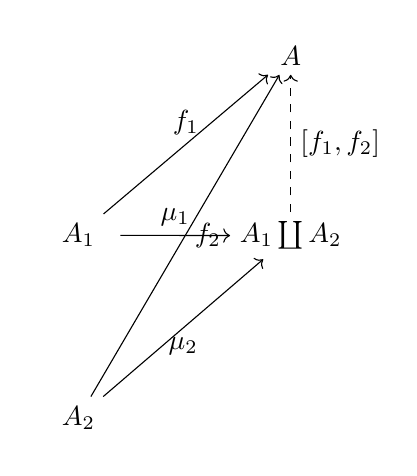
\begin{tikzpicture}
\matrix (m) [matrix of math nodes, row sep=5em, column sep=4em, minimum width=3em]
{
	& A  \\ 
	A_1  &  A_1 \coprod A_2   \\
	A_2 & \\
};
\path[->]
(m-2-1) edge node [above] {$f_1$} (m-1-2)
edge node [above] {$\mu_1$} (m-2-2)
(m-3-1) edge node [right] {$f_2$} (m-1-2)
edge node [below] {$\mu_2$} (m-2-2)
;
\path[dashed,->]
(m-2-2) edge node [right] {$[f_1,f_2]$} (m-1-2)
;
\end{tikzpicture}
\end{gathered}
\end{equation}

So to generalized, for $i\in I$, (finite set $I$?)

\textbf{coproduct} $(\mu_j, \coprod_{i\in I} A_i)_{j\in I}$, where \\
(family of) injection (morphisms) $\mu_j : A_j \to \coprod_{i \in I } A_i$

s.t.

\[
\forall \, A \in \text{Obj}\mathbf{A}, \, \forall \, f_i \in \text{Mor}\mathbf{A}, \, i \in I, \, f_i : A_i \to A
\]
then
\begin{equation}
\begin{gathered}
\exists \, ! \, [f_i ] \equiv [f_i]_{i\in I} \in \text{Mor}\mathbf{A} , \, [f_i] : \coprod_{i\in I} A_i \to A \text{ s.t. } \\ 
[f_i] \mu_j = f_j \qquad \, \forall \, j \in I
\end{gathered}
\end{equation}
i.e.

\begin{equation}
\begin{gathered}
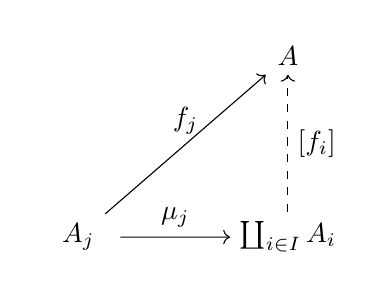
\begin{tikzpicture}
\matrix (m) [matrix of math nodes, row sep=5em, column sep=4em, minimum width=3em]
{
	& A  \\ 
	A_j  & \coprod_{i\in I} A_i   \\
};
\path[->]
(m-2-1) edge node [above] {$f_j$} (m-1-2)
edge node [above] {$\mu_j$} (m-2-2)
;
\path[dashed,->]
(m-2-2) edge node [right] {$[f_i]$} (m-1-2)
;
\end{tikzpicture} 
\end{gathered}
\end{equation}



For notation purposes only, recall that it's denoted the sets $\text{Hom}(A,B)$ in ${}_R\textbf{Mod}$ by
\[
\text{Hom}_R(A,B)
\]
i.e., in my notation, for $A,B \in \text{Obj}{ {}_R \textbf{Mod}}$, $\text{Hom}(A,B) \subset \text{Mor}( {}_R\textbf{Mod})$, $\text{Hom}(A,B) \equiv \text{Hom}_R(A,B)$

\begin{definition}[pre-additive category] 
	category $\mathbf{C}$ is \textbf{pre-additive} if $\forall \,  \text{Hom}(A,B)$, $\text{Hom}(A,B)$ equipped with binary operation $+$ s.t. $\forall \, f,g  \in \text{Hom}(A,B)$, 
	\begin{enumerate}
		\item if $p: B\to B'$, then 
		\[
		p(f+g) = pf + pg \in \text{Hom}(A,B')
		\]
		\item if $q: A'\to A$, then 
		\[
		(f+g)q = fq + gq \in \text{Hom}(A',B)
		\]
		and 
		\[
		f+g= g+f \qquad \, \text{ (additive abelian) }
		\] 
	\end{enumerate}
\end{definition}

\subsubsection{Examples of extra assumptions on sets, ${}_R\textbf{Mod}$ we take for granted}

In Prop. 7.15(iii) Rotman (2010) \cite{JRotman2010}, \\
direct sum $M=A\oplus B$ if $\exists \, $ homomorphisms $\begin{aligned} & \quad \\
& p:M\to A \\
& q:M\to B \\
& i:A\to M \\
& j:B\to M \end{aligned}$ s.t. $\begin{aligned} & \quad \\
& pi = 1_A \\
& qj = 1_B \\ 
& pj = 0 \\ & qi = 0 \end{aligned}$, 
\[
ip + jq = 1_M
\]
direct sum $M = A\oplus B$ uses property that morphisms can be added ${}_R\textbf{Mod}$ has this property. $\textbf{Sets}$ don't.  

In Corollary 7.17, \\
direct sum in terms of arrows, \\
$\exists \, $ map $\rho:M \to S$ s.t. $\rho(s)=s$.  Moreover $\text{ker}\rho = \text{im}j$, $\text{im}\rho = \text{im}i$ and $\rho(s)=s$, \, $\forall \, s \in \text{im}\rho$.  

\begin{tikzpicture}
\matrix (m) [matrix of math nodes, row sep=5em, column sep=4em, minimum width=3em]
{
	S & M & T \\ 
};
\path[->]
(m-1-1) edge node [above] {$i$} (m-1-2)
(m-1-3) edge node [above] {$j$} (m-1-2)
;
\end{tikzpicture} 
and $M\simeq S \coprod T$, \\
where $\begin{aligned} & \quad \\
& i: s \mapsto s \\ 
& j : t \mapsto t \end{aligned}$ (i.e. inclusions)

This makes sense in $\textbf{Sets}$, but doesn't make sense in arbitrary categories because image of morphism may fail, e.g. $\text{Mor}(\mathcal{C}(G))$ are elements in $\text{Hom}(*,*) =G$, not functions.  

Categorically, object $S$ is (equivalent to) retract of object $M$, $S,M \in \text{Obj}\mathbf{C}$, if $\exists \, $ morphisms $i,p\in \text{Mor}(\mathbf{C})$, s.t. 
\[
\begin{aligned}
& i: S\to M \\
& p:M \to S 
\end{aligned}
\]
s.t. $pi=1_S$, $(ip)^2=ip$ (for modules, define $\rho = ip$)

\begin{definition}[free products]
	\textbf{free products} are coproducts in groups
\end{definition}

Prop. 7.26, Rotman (2010) \cite{JRotman2010}
\begin{proposition}[7.26, Rotman]
	If $A,B$ are $R$-modules, \\
	then their coproducts in ${}_R\textbf{Mod}$ exists, and it's the direct sum $C= A\coprod B$.  
\end{proposition}

\begin{proof}
	Define 
	\[
	\begin{gathered}
	\begin{aligned}
	& \mu : A \to C \\
	& \mu : a \mapsto (a,c)
	\end{aligned}
	\qquad \, 
	\begin{aligned}
	& \nu : B \to C \\
	& \nu : b \mapsto (0,b)
	\end{aligned} \qquad \, \text{ (Rotman's notation) } \begin{aligned}
	& \alpha : A \to C \\
	& \beta : B\to C 
	\end{aligned}
	\end{gathered}
	\]
	Let $X$ be a module, $f:A\to X$, $g:B\to X$ homomorphisms
\end{proof}

Define 
\[
\begin{aligned}
& \theta : C \to X \\ 
& \theta: (a,b) \mapsto f(a) + g(b)
\end{aligned}
\]
\[
\begin{aligned}
& \theta \mu (a) = \theta(a,0) = f(a) \\ 
&  \theta\nu (b) = \theta(0,b)  = g(b)
\end{aligned}
\]
so diagram commutes, i.e. 

\[
\begin{gathered}
\begin{tikzpicture}
\matrix (m) [matrix of math nodes, row sep=5em, column sep=4em, minimum width=3em]
{
	& X  & \\ 
	A  & C & B   \\
};
\path[->]
(m-2-1) edge node [above] {$f$} (m-1-2)
edge node [above] {$\mu$} (m-2-2)
(m-2-3) edge node [above] {$g$} (m-1-2)
edge node [above] {$\nu$} (m-2-2)
;
\path[dashed,->]
(m-2-2) edge node [right] {$\theta$} (m-1-2)
;
\end{tikzpicture} 
\end{gathered}
\]

If $\psi: C\to X$ makes diagram commute, 
\[
\begin{aligned}
& \psi((a,0)) = f(a) \qquad \, \forall \, a\in A \\
& \psi((0,b)) = g(b) \qquad \, \forall \, b\in B \\
\end{aligned}
\]
and since $\psi$ is a homomorphism, $\psi((a,b)) = \psi((a,0)) + \psi((0,b)) = f(a) + g(b)  = \theta((a,b))$.  $\psi = \theta$.  

Prop. 7.27, Rotman (2010) \cite{JRotman2010}
\begin{proposition}[7.27, Rotman]
	If category $\mathcal{C} = \mathbf{C}$, and if $A,B \in \text{Obj}\mathbf{C}$, then $\forall \, $ 2 coproducts of $A,B$, if they $\exists \, $, are equivalent.  
\end{proposition}
\begin{proof}
	Suppose $C,D$ coproducts of $A,B$.  Suppose coproducts $\begin{aligned} & \quad \\ 
	& \mu_A : A \to C , \qquad \, & \nu_A: A\to D \\
	& \mu_B : B \to C , \qquad \, & \nu_B : B \to D \end{aligned}$  
	\[
	\begin{gathered}
	\begin{tikzpicture}
	\matrix (m) [matrix of math nodes, row sep=5em, column sep=4em, minimum width=3em]
	{
		& D  & \\ 
		A  & C & B   \\
	};
	\path[->]
	(m-2-1) edge node [above] {$\nu_A$} (m-1-2)
	edge node [above] {$\mu_A$} (m-2-2)
	(m-2-3) edge node [above] {$\nu_B$} (m-1-2)
	edge node [above] {$\mu_B$} (m-2-2)
	;
	\path[dashed,->]
	(m-2-2) edge node [right] {$\theta$} (m-1-2)
	;
	\end{tikzpicture} 
	\end{gathered}
	\]
	Just substitute $X=D$ in diagram above.  
	
	Then substitute again: 
	\[
	\begin{gathered}
	\begin{tikzpicture}
	\matrix (m) [matrix of math nodes, row sep=5em, column sep=4em, minimum width=3em]
	{
		& C  & \\ 
		A  & D & B   \\
	};
	\path[->]
	(m-2-1) edge node [above] {$\mu_A$} (m-1-2)
	edge node [above] {$\nu_A$} (m-2-2)
	(m-2-3) edge node [above] {$\mu_B$} (m-1-2)
	edge node [above] {$\nu_B$} (m-2-2)
	;
	\path[dashed,->]
	(m-2-2) edge node [right] {$\psi$} (m-1-2)
	;
	\end{tikzpicture} 
	\end{gathered}
	\]
	Then combine the 2 diagrams: $\psi \theta = 1_C$.  Likewise by label symmetry of $C,D$, $\theta \psi = 1_D$.  
	
	Then $C,D$ are equivalent.  
\end{proof}


Exer. 7.29 on pp. 459 of Rotman (2010) \cite{JRotman2010}

\begin{definition}
	If $A,B\in \text{Obj}\mathbf{C}$, then their \textbf{product}; $A\prod B = P \in \text{Obj}\mathbf{C}$, and morphisms $\begin{aligned} & \quad \\ 
	& p : P \to A \\ 
	& q : P \to B \end{aligned}$  s.t. $\forall \, X \in \text{Obj}\mathbf{C}$, \, $\forall \, \begin{aligned} & \quad \\ 
	& f : X \to A \in \text{Mor}\mathbf{C} \\ 
	& g : X \to B \in \text{Mor}\mathbf{C} \end{aligned}$, \\
	$\exists \, ! \, \theta:X \to P$, s.t. 
	
	\[
	\begin{gathered}
	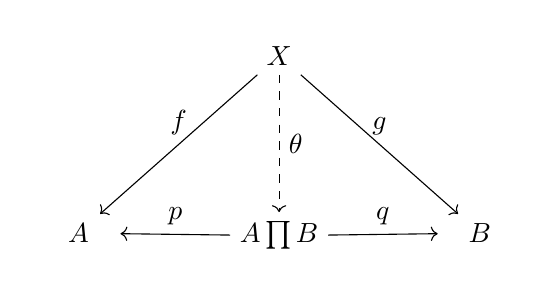
\begin{tikzpicture}
	\matrix (m) [matrix of math nodes, row sep=5em, column sep=4em, minimum width=3em]
	{
		& X  & \\ 
		A  & A \prod B & B   \\
	};
	\path[->]
	(m-1-2) edge node [above] {$f$} (m-2-1)
	edge node [above] {$g$} (m-2-3)
	(m-2-2) edge node [above] {$p$} (m-2-1)
	edge node [above] {$q$} (m-2-3)
	;
	\path[dashed,->]
	(m-1-2) edge node [right] {$\theta$} (m-2-2)
	;
	\end{tikzpicture} 
	\end{gathered}
	\]
	
	If the notation of Kashiwara and Schapira (2006) \cite{KaSch2006}, 
	\[
	\begin{gathered}
	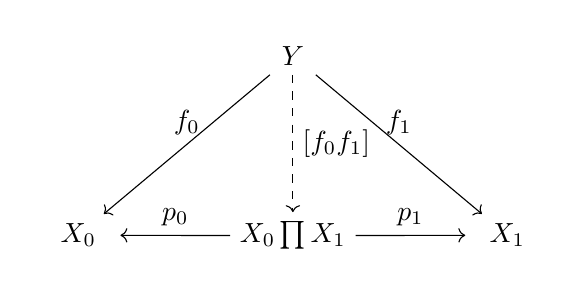
\begin{tikzpicture}
	\matrix (m) [matrix of math nodes, row sep=5em, column sep=4em, minimum width=3em]
	{
		& Y  & \\ 
		X_0  & X_0 \prod X_1 & X_1   \\
	};
	\path[->]
	(m-1-2) edge node [above] {$f_0$} (m-2-1)
	edge node [above] {$f_1$} (m-2-3)
	(m-2-2) edge node [above] {$p_0$} (m-2-1)
	edge node [above] {$p_1$} (m-2-3)
	;
	\path[dashed,->]
	(m-1-2) edge node [right] {$[f_0f_1]$} (m-2-2)
	;
	\end{tikzpicture} 
	\end{gathered}
	\]
	In general
	\[
	\begin{gathered}
	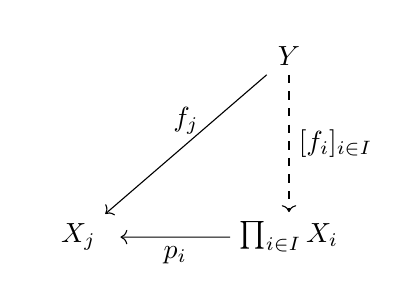
\begin{tikzpicture}
	\matrix (m) [matrix of math nodes, row sep=5em, column sep=4em, minimum width=3em]
	{
		& Y  \\ 
		X_j  & \prod_{i\in I} X_i   \\
	};
	\path[->]
	(m-1-2) edge node [above] {$f_j$} (m-2-1)
	(m-2-2) edge node [below] {$p_i$} (m-2-1)
	;
	\path[dashed,->]
	(m-1-2)        edge node [right] {$[f_i]_{i\in I}$} (m-2-2)
	;
	\end{tikzpicture}  
	\end{gathered}
	\]
	
	\textbf{product} of $X_i$'s, 
	\[ 
	\prod_i X_i \equiv \prod_{i\in I} X_i
	\]
	given by 
	\begin{equation}
	\prod_i X_i := \lim_{ \longleftarrow } \alpha 
	\end{equation}
	
	When $X_i = X$, $\forall \, i \in I$, denote product by $X^{ \prod I} \equiv X^I$.  
	
	
\end{definition}

e.g. Cartesian product $P= A\times B$ of 2 sets $A,B$, $A,B \in \text{Obj}\textbf{Sets}$.  

Define 	
\[
\begin{gathered}
\begin{aligned}
& p:A\times B \to A \\
& p(a,b) \mapsto a 
\end{aligned} \qquad \, 
\begin{aligned}
& q:A\times B \to B \\
& q(a,b) \mapsto b 
\end{aligned}
\end{gathered}
\]
If $X \in \text{Obj}\textbf{Sets}$,  \\
if 
$	\begin{aligned} & \quad \\ 
& f: X \to A \\
& g : X  \to B 
\end{aligned}
$, then $\begin{aligned} & \quad \\ 
& \theta: X \to A\times B \\
& \theta : x \mapsto (f(x),g(x)) \in A\times B
\end{aligned}
$

\begin{proposition}[7.28 Rotman (2010); equivalence of products, if it exists]
	If $A,B \in \text{Obj}\mathbf{C}$, then $\forall \, $ 2 products of $A$ and $B$, should they exist, are equivalent. 
\end{proposition}

\begin{proof}
	Suppose $C,D$ products of $A,B$.  Suppose products $\begin{aligned} & \quad \\ 
	& p_A : C \to A , \qquad \, & q_A: D\to A \\
	& p_B : C \to B , \qquad \, & q_B : D \to B \end{aligned}$  
	\[
	\begin{gathered}
	\begin{tikzpicture}
	\matrix (m) [matrix of math nodes, row sep=5em, column sep=4em, minimum width=3em]
	{
		& D  & \\ 
		A  & C & B   \\
	};
	\path[->]
	(m-1-2) edge node [above] {$q_A$} (m-2-1)
	edge node [above] {$q_B$} (m-2-3)
	(m-2-2) edge node [above] {$p_A$} (m-2-1)
	edge node [above] {$p_B$} (m-2-3)
	;
	\path[dashed,->]
	(m-1-2) edge node [right] {$\theta$} (m-2-2)
	;
	\end{tikzpicture} 
	\end{gathered}
	\]
	Just substitute $X=D$ in diagram above.  
	
	Then substitute again: 
	\[
	\begin{gathered}
	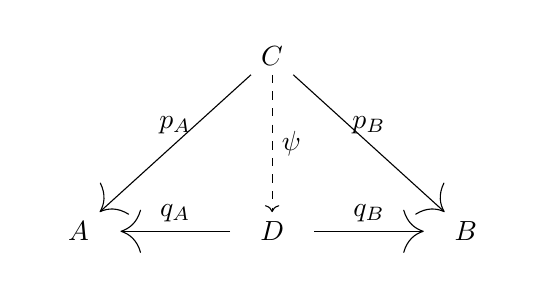
\begin{tikzpicture}
	\matrix (m) [matrix of math nodes, row sep=5em, column sep=4em, minimum width=3em]
	{
		& C  & \\ 
		A  & D & B   \\
	};
	\path[-{>[scale=3.0]}]
	(m-1-2) edge node [above] {$p_A$} (m-2-1)
	edge node [above] {$p_B$} (m-2-3) 
	(m-2-2) edge node [above] {$q_A$} (m-2-1)
	edge node [above] {$q_B$} (m-2-3)
	;
	\path[dashed,->]
	(m-1-2) edge node [right] {$\psi$} (m-2-2)
	;
	\end{tikzpicture} 
	\end{gathered}
	\]
	Then combine the 2 diagrams: $\psi \theta = 1_C$.  Likewise by label symmetry of $C,D$, $\theta \psi = 1_D$.  
	
	Then $C,D$ are equivalent.  
	
	
\end{proof}

\subsubsection{Products of Modules and Sets}  

\begin{proposition}[7.29 Rotman (2010); products of R-modules are equivalent]
	If commutative ring $R$, \\
	R-modules $A,B$, \\
	then $\exists \, $ their (categorical) product $A\sqcup B$, in fact 
	\begin{equation}
	A \sqcap B \cong A\sqcup B
	\end{equation}
	
\end{proposition}

\begin{proof}
	If $A\sqcup B \cong M$, then 
	$\exists \, $ R-maps, $\begin{aligned} & \quad \\
	& i : S\to M \\ 
	& j : T \to M \end{aligned}$, \qquad \,  $\begin{aligned} & \quad \\
	& p : M\to S \\ 
	& q : M \to T \end{aligned}$
	s.t. $\begin{aligned} & \quad \\
	& pi = 1_A \\ 
	& qj = 1_B \end{aligned}$ \qquad \, and $\begin{aligned} & \quad \\
	& pj = 0 \\ 
	& qi = 0 \end{aligned}$, and $ip + jq = 1_M$, i.e.   
	
	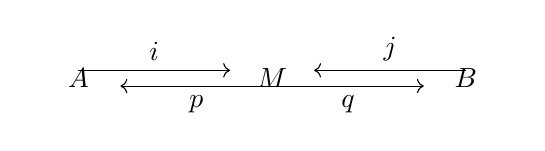
\begin{tikzpicture}
	\matrix (m) [matrix of math nodes, row sep=5em, column sep=4em, minimum width=3em]
	{
		A & M & B \\ 
	};
	\path[->]
	($(m-1-2)+(0,-0.1)$) edge node [below] {$p$} ($(m-1-1.east)+(0,-0.1)$)
	edge node [below] {$q$} ($(m-1-3.west)+(0,-0.1)$) 
	($(m-1-1)+(0,0.1)$) edge node [above] {$i$} ($(m-1-2.west)+(0,0.1)$)
	($(m-1-3)+(0,0.1)$) edge node [above] {$j$} ($(m-1-2.east)+(0,0.1)$)
	;
	\end{tikzpicture} 
	
	If module $X$, since $\begin{aligned}
	& \quad \\ 
	& f: X \to A \\
	& g:X\to B
	\end{aligned}	$ 
	are homomorphisms, 
	
	define 
	$\begin{aligned}
	& \theta: X \to A \sqcup B \\
	& \theta(x) = if(x) + jg(x)
	\end{aligned}
	$
	so that 
	\[
	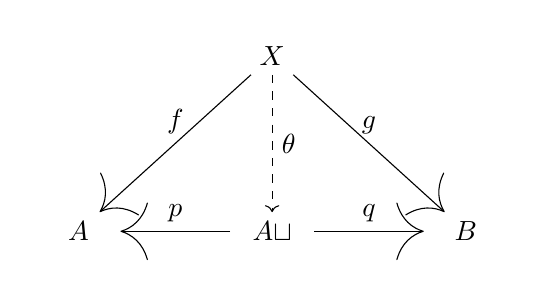
\begin{tikzpicture}
	\matrix (m) [matrix of math nodes, row sep=5em, column sep=4em, minimum width=3em]
	{
		& X  & \\ 
		A  & A\sqcup  & B   \\
	};
	\path[-{>[scale=4.0]}]
	(m-1-2) edge node [above] {$f$} (m-2-1)
	edge node [above] {$g$} (m-2-3) 
	(m-2-2) edge node [above] {$p$} (m-2-1)
	edge node [above] {$q$} (m-2-3)
	;
	\path[dashed,->]
	(m-1-2) edge node [right] {$\theta$} (m-2-2)
	;
	\end{tikzpicture} 
	\]
	since, $\forall \, x \in X$, 
	\[
	p\theta(x) = pif(x) + pjg(x) = pif(x) + 0 = f(x)
	\]
	since $ip + jq=1_{A\sqcup B}$  
	
	\[
	\psi = ip\psi + jq \psi = i f + jf = \theta
	\]
	so product is unique.  
\end{proof}

\begin{definition}
	Let $R$ be commutative ring, \\
	let $\lbrace A_i : i \in I \rbrace$ be indexed family of $R$-modules.  
	
	\textbf{direct product} $\prod_{i\in I} A_i$ is cartesian product (i.e. set of all $I$-tuples $(a_i)$ whose $i$th coordinate $a_i$ lies in $A_i \quad \, \forall \, i$) with coordinate wise addition and scalar multiplication: 
	\[
	\begin{gathered}
	(a_i) + (b_i) = (a_i + b_i) \\
	r(a_i) = (ra_i)
	\end{gathered}
	\]
	where $r\in R$, $a_i, b_i \in A_i$, \, $\forall \, i $  
\end{definition}




cf. Thm. 7.32 of Rotman (2010) \cite{JRotman2010}
\begin{theorem}[7.32, Rotman]
	Let commutative ring $R$.  \\
	$\forall \, R$-module $A$, $\forall \,$ family $\lbrace B_i | i \in I \rbrace$ of $R$-modules,
	\begin{equation}
	\begin{gathered}
	\text{Hom}_R(A, \coprod_{i\in I} B_i ) \simeq \coprod_{i \in I} \text{Hom}_R(A,B_i)
	\end{gathered}
	\end{equation}
	via $R$-isomorphism
	\[
	\varphi : f\mapsto (p_if)
	\]
	where $p_i $ are projections of product $\coprod_{i\in I }B_i$
\end{theorem}

\begin{proof}
	Let $a\in A$, $f,g \in \text{Hom}_R(A,\coprod_{i\in I} B_i)$.
	\[
	\varphi(f+g)(a) = (p_i(f+g))(a) = (p_i(f(a) + g(a))) = (p_if + p_ig)(a)
	\]
	$\varphi$ additive.
	
	$\forall \, i, \, \forall \, r \in R$, $p_i rf = rp_i f$ (since product of $R$-modules, $\coprod_{i\in I}B_i$ is also an $R$-module of $\text{Obj}{}_R\textbf{Mod}$, by def. of product).
	\[
	\varphi rf \mapsto (p_i rf) = (r p_i f) = r(p_i f) = r\varphi(f)
	\]
	So $\varphi$ is $R$-map.
	
	If $(f_i) \in \coprod_i \text{Hom}{}_R(A,B_i)$, then $f_i : A\to B_i$ \, $\forall \, i$
	
	By Rotman's Prop. 7.31 (If family of $R$-modules $\lbrace A_i | i \in I \rbrace$, then direct product $C = \coprod_{i\in I} A_i$ is their product in ${}_R \textbf{Mod}$), \\
	\phantom{ \qquad \, } By def. or product, $\exists \, ! \, R$-map , \, $\theta : A \to \coprod_{i\in I} B_i$ s.t. $p_i \theta = f_i$ \, $\forall \, i$
	
	\[
	\begin{gathered}
	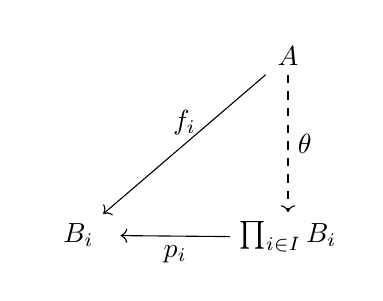
\begin{tikzpicture}
	\matrix (m) [matrix of math nodes, row sep=5em, column sep=4em, minimum width=3em]
	{
		& A  \\ 
		B_i  & \prod_{i\in I} B_i   \\
	};
	\path[->]
	(m-1-2) edge node [above] {$f_i$} (m-2-1)
	(m-2-2) edge node [below] {$p_i$} (m-2-1)
	;
	\path[dashed,->]
	(m-1-2)        edge node [right] {$\theta$} (m-2-2)
	;
	\end{tikzpicture}  
	\end{gathered}
	\]
	
	
	
	
	Then 
	\[
	f_i) = (p_i\theta) = \varphi(\theta)
	\]
	, and so $\varphi$ \emph{surjective}.
	
	Suppose $f\in \text{ker}\varphi$, so $\theta = \varphi(f) = (p_if)$.  Thus $p_i f=0$ \, $\forall \, i$
	
	\[
	\begin{gathered}
	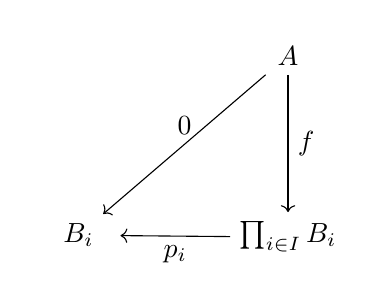
\begin{tikzpicture}
	\matrix (m) [matrix of math nodes, row sep=5em, column sep=4em, minimum width=3em]
	{
		& A  \\ 
		B_i  & \prod_{i\in I} B_i   \\
	};
	\path[->]
	(m-1-2) edge node [above] {$0$} (m-2-1)
	edge node [right] {$f$} (m-2-2)
	(m-2-2) edge node [below] {$p_i$} (m-2-1)
	;
	\end{tikzpicture}  
	\end{gathered}
	\]
	
	But $0$-homomorphism also makes this diagram commute, so uniqueness of homomorphism $A \to \prod B_i$ gives $f=0$.  
	
	
	
	
\end{proof}



%--------------------------------------------------------------------------------
% END of 20180202 
%-------------------------------------------------------------------------------

\section{Applications of Category Theory: Finite State Machines (FSM)}

\begin{definition}[Finite State Machines $\equiv$ Finite State Automaton]
	A deterministic finite state machine or acceptor deterministic finite state machine is a quintuple ($\Sigma, S, s_0, \delta F$) where \\
	$\Sigma \equiv $ input alphabet (finite, non-empty set of symbols) \\
 	$S \equiv $ finite, non-empty set of states \\
 	$s_0 \equiv $ initial state, $s_0 \in S$ \\
 	$\delta \equiv $ state-transition function; $\delta : S \times \Sigma \to S$ (in a nondeterministic finite automaton, it would be $\delta : S \times \Sigma \to \mathcal{P}(S)$), i.e. $\delta$ would return a set of states; $\mathcal{P}(S) \equiv $ set of all subsets of $S$, including $\emptyset$ and $S \equiv$ power set. \\
 	$F \equiv $ set of final states, (possibly empty subset of $S$; $F\subseteq S$ or $F \subseteq S \cup \lbrace \emptyset \rbrace$)

	Finite State Machine (FSM) is also known as a Finite State Automaton.
\end{definition}
cf. \href{https://xlinux.nist.gov/dads/HTML/finiteStateMachine.html}{Black, Paul E (12 May 2008). "Finite State Machine". \emph{Dictionary of Algorithms and Data Structres}}. U.S. National Institute of Standards and Technology (NIST).

For both deterministic and non-deterministic FSMs, it's conventional to allow $\delta$ to be a partial function, i.e. 
$\delta(q,x)$ doesn't have to be defined for every combination of $q \in S$, $x \in \Sigma$

If FSM $M$ is in state $q$; the next symbol (input?) is $x$ and $\delta(q,x)$ not defined; then $M$ can announce an error (i.e. reject the input (???)). 


\begin{definition}[Alphabet]
	alphabet $:= $ nonempty set of symbols $\equiv \Sigma$ \\
	string $:=$ finite sequence of members (i.e. symbols) of an underlying base set (i.e. \textbf{alphabet}) \\
	$\Sigma^n \equiv $ set of all strings of length $n$.
\end{definition}

\part{Category Theory}

\section{Note on notation}

From the section on ``Terminology'' of the Preface of Barr and Wells (1998) \cite{BW1998}:

\begin{quote}
	``In most scientific disciplines, notation and terminology are standardized, of- ten by an international nomenclature committee. (Would you recognize Einstein’s equation if it said $p = HU^2$?) We must warn the nonmathematician reader that such is not the case in mathematics. There is no standardization body and terminology and notation are individual and often idiosyncratic.''
\end{quote}

To try to bridge the difference choice of notation and through comparison, suggest the ``best'' notation that's easy to remember and easy to use, I'll present all the different types of notation that I come across as much as I can. My plan of attack is the following:
\begin{enumerate}
	\item I'll try to present different types of notation and reference the authors of the text when I can.
	\item I'll try to defer to the notation used in Wikipedia, first.
	\item I'll make a final decision of what notation works best (for me).
\end{enumerate}

\section{Category $\mathbf{A}$, (definition)}

\begin{definition}[Category $\mathbf{A}$]
\textbf{category} $\mathbf{A}$ is quadruple $\mathbf{A} = (\text{Obj}(\mathbf{A}), \text{Mor}\mathbf{A}, 1,\circ)$ 
\begin{equation}
\mathbf{A} = (\text{Obj}(\mathbf{A}), \text{Mor}\mathbf{A}, 1,\circ)
\end{equation}
s.t.
\begin{enumerate}
	\item $\text{Obj}{(\mathbf{A})}$ is a \emph{class}, whose elements, $A \in \text{Obj}(\mathbf{A})$, are called \emph{objects}
	\item $\text{Mor}\mathbf{A}$ is a \emph{class}.
	\begin{enumerate}
		\item From Ad\'{a}mek, Herrlich, and Strecker (2004) \cite{AHS2004}, Kashiwara and Schapira (2006) \cite{KaSch2006}, \\
		$\forall \, A, B \in \text{Obj}(\mathbf{A})$, $\exists \, \text{Hom}(A,B) \subseteq \text{Mor}(\mathbf{A})$. Therefore, 
		\begin{equation}
		\text{Mor}\mathbf{A} = \bigcup_{ A,B \in \text{Obj}(\mathbf{A}) } \text{Hom}(A,B)
		\end{equation}
		\item $\forall \, f \in \text{Hom}(A,B)$, $f: A \to B \in \text{Hom}(A,B)$ is a \emph{morphism}. 
	\[
\begin{tikzpicture}
\matrix (m) [matrix of math nodes, row sep=3em, column sep=4em, minimum width=2em]
{
	A & B  \\
};
\path[->]
(m-1-1) edge node [above] {$f$} (m-1-2)
;
\end{tikzpicture}
\]
	\end{enumerate}
	\item $\forall \, A \in \text{Obj}(\mathbf{A})$, $\exists \, 1_A : A \to A$, i.e. $\exists \, \mathbf{1}_A \in \text{Hom}_{\mathbf{A}}(A,A) \equiv \text{Hom}(A,A)$, 
	\[
	\begin{tikzpicture}
	\matrix (m) [matrix of math nodes, row sep=3em, column sep=4em, minimum width=2em]
	{
		A & A  \\
	};
	\path[->]
	(m-1-1) edge node [above] {$1_A$} (m-1-2)
	;
	\end{tikzpicture} \text{ or } 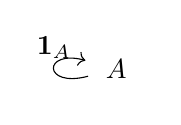
\begin{tikzpicture}
	\matrix (m) [matrix of math nodes, row sep=3em, column sep=4em, minimum width=2em]
	{
		A   \\
	};
	\path[->]
	(m-1-1) edge [loop left] node [above] {$\mathbf{1}_A$} (m-1-1)
	;
	\end{tikzpicture}
	\]
	\item \textbf{composition:} 
	$\forall \, A,B,C \in \text{Obj}\mathbf{A}$, define \textbf{composition} to be a map
	\begin{equation}
	\begin{aligned}
		\text{Hom}_{\mathbf{A}}(A, B) \times \text{Hom}_{\mathbf{A}}(B, C) & \to \text{Hom}_{\mathbf{A}}(A, C) \\
		 (f, g) & \mapsto g\circ f
 	\end{aligned}
\end{equation}, i.e.
	
	$\forall \, \begin{aligned} & \quad \\
	& f: A \to B \in \text{Hom}(A,B) \\
	& g:B\to C \in \text{Hom}(B,C) \end{aligned}$, i.e. $f,g \in \text{Mor}\mathbf{A}$, \\
	then $g\circ f : A \to C \in \text{Hom}(A,C)$, $g\circ f \in \text{Mor}\mathbf{A}$ i.e. 
	\[
	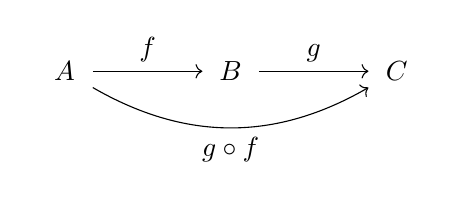
\begin{tikzpicture}
	\matrix (m) [matrix of math nodes, row sep=3em, column sep=4em, minimum width=2em]
	{
		A & B & C  \\
	};
	\path[->]
	(m-1-1) edge node [above] {$f$} (m-1-2)
	(m-1-2) edge node [above] {$g$} (m-1-3)
	(m-1-1) edge [bend right=30] node [below] {$g\circ f$} (m-1-3) 
	;
	\end{tikzpicture}
	\]
	s.t. 
	\begin{enumerate}
		\item \emph{associativity} $\forall \, \begin{aligned} & \quad \\
		& f: A \to B \\
		& g: B \to C \\
		& h: C \to D \end{aligned}$, $h\circ (g\circ f) = (h\circ g) \circ f $ i.e.
		
		\[
		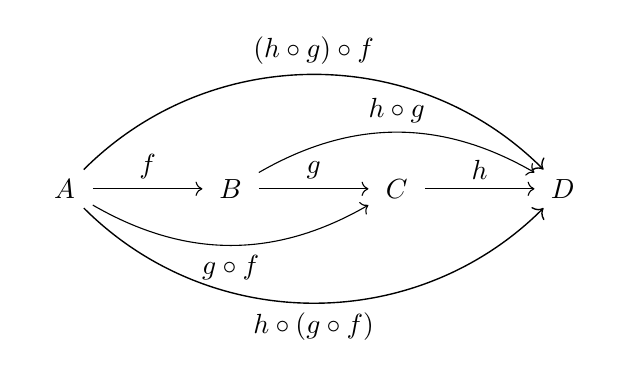
\begin{tikzpicture}
		\matrix (m) [matrix of math nodes, row sep=3em, column sep=4em, minimum width=2em]
		{
			A & B & C  & D \\
		};
		\path[->]
		(m-1-1) edge node [above] {$f$} (m-1-2)
		(m-1-2) edge node [above] {$g$} (m-1-3)
		(m-1-3) edge node [above] {$h$} (m-1-4)
		(m-1-1) edge [bend right=30] node [below] {$g\circ f$} (m-1-3) 
		(m-1-2) edge [bend left=30] node [above] {$h\circ g$} (m-1-4) 
		;
		\path[-{>[scale=1.15]}, line width=0.5pt]
		(m-1-1) edge [bend left=45] node [above] {$(h \circ g)\circ f$} (m-1-4)
		edge [bend right=45] node [below] {$h \circ (g\circ f)$} (m-1-4);
		\end{tikzpicture}
		\]
		
		\item $\forall \, f:A \to B \in \text{Hom}(A,B)$, $1_B \circ f = f $ and $f\circ 1_A = f$ i.e.
		
		$\forall \, f \in \text{Hom}_{\mathbf{A}}(A,B)$,
		\[
		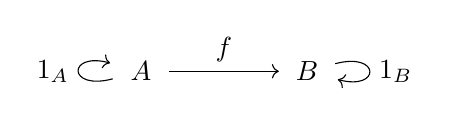
\begin{tikzpicture}
		\matrix (m) [matrix of math nodes, row sep=3em, column sep=4em, minimum width=2em]
		{
			A & B  \\
		};
		\path[->]
		(m-1-1) edge node [above] {$f$} (m-1-2)
		edge [loop left] node [left] {$1_A$} (m-1-1)
		(m-1-2) edge [loop right] node [right] {$1_B$} (m-1-2)
		;
		\end{tikzpicture}
		\]
		\item Ad\'{a}mek, Herrlich, and Strecker (2004) \cite{AHS2004} posited further that $\text{Hom}(A,B) \in \text{Mor}\mathbf{A}$ pairwise disjoint (i.e. $\text{Hom}(A,B) \bigcap \text{Hom}(C,D) \neq \emptyset$ if $C\neq A$ or $D\neq B$)
	\end{enumerate}
\end{enumerate}	
\end{definition}

\subsection{Examples}

\begin{itemize}
	\item $\textbf{Set} = (\text{Obj}{(\textbf{Set})}, \text{Hom}{\textbf{Set}},\mathbf{1},\circ)$ where \\
	$\text{Obj}{(\textbf{Set})}$ is the class of all sets \\
	$\text{Hom}{\textbf{Set}}$ is the class of all functions on a set to another set
	\item $\textbf{Vec}$
	
	\[
	\begin{aligned}
	& \text{Obj}\textbf{Vec} & \equiv \text{ all real vector spaces } \\ 
	& \text{Mor}\textbf{Vec} & \equiv \text{ all linear transformations between them (between real vector spaces) }
	\end{aligned}
	\]
	
	\item \textbf{Monoid}.  Consider a monoid as a triple $(M, \cdot, e)$.  \\
	Every semigroup $(M,\cdot)$ (recall that a \emph{semigroup} is a set $S$ with binary operation $\cdot $, i.e. s.t.
	
	\quad \,  $\begin{aligned} & \quad \\
	& S\times S \xrightarrow{\cdot } S \\ 
	& \forall \, a,b ,c \in S, \, (a\cdot b)\cdot c = a\cdot (b\cdot c) \quad \, \text{ (associativity) } \end{aligned}$ 
	
	\quad \, (but no inverse, necessarily!)) that also has a unit $e$ can be made into a category $\mathbf{C}$ 
	
	$\Longrightarrow \mathbf{C}(M,\cdot ,e) = (\text{Obj}(\mathbf{C}), \text{Hom}(\mathbf{C}), \mathbf{1}, \circ)$, a category $\mathbf{C}$ with only 1 object, i.e. $\text{Obj}(\mathbf{C}) = \lbrace M \rbrace$, so that \\
	$\text{Obj}(\mathbf{C}) = \lbrace M \rbrace$ \\
	$\text{Hom}(M,M) = M$ \\
	$\mathbf{1}_M = e$ \\
	$y \circ x = y \cdot x$
\end{itemize}

\subsection{Duality, opposite category}

Given a category $\mathbf{A} = ( \text{Ob}, \text{hom}_{\mathbf{A}}, 1, \circ)$, 
\begin{definition}[dual opposite category]
	\textbf{dual} or \textbf{opposite} category of $\mathbf{A} = (\text{Obj}(\mathbf{A}), \text{Mor}\mathbf{A}, \mathbf{1}, \circ)$, denoted $\mathbf{A}^{\text{op}}$, is   
	\begin{equation}
	\mathbf{A}^{\text{op}}  =  (\text{Obj}(\mathbf{A}), \text{Mor}\mathbf{A}^{\text{op}}, \mathbf{1}, \circ^{\text{op}})
	\end{equation}
	s.t.
\begin{itemize}
	\item 
	\begin{equation}
	\text{Obj}(\mathbf{A}^{\text{op}}) = \text{Obj}(\mathbf{A})
	\end{equation}
	\item $\forall \, A, B \in \text{Obj}(\mathbf{A}^{\text{op}})$, $\text{Hom}_{\mathbf{A}^{\text{op}}}(A,B) \subseteq \text{Mor}\mathbf{A}^{\text{op}}$, 
		\begin{equation}
\text{Hom}_{\mathbf{A}^{\text{op}}}(A,B) = \text{Hom}_{\mathbf{A}}(B,A) \subseteq \text{Mor}\mathbf{A}
		\end{equation}
		\item \emph{Define} the new composition 
		\begin{equation}
\begin{gathered}
		f \circ^{\text{op}} g \text{ of } \begin{aligned} & \quad \\
		& g \in \text{Hom}_{\mathbf{A}^{\text{op}}}(C,B) \\
		& f \in \text{Hom}_{\mathbf{A}^{\text{op}}}(B,A) 
		\end{aligned}		 \\
		\text{ then } \\
		f \circ^{\text{op}} g = g\circ f
\end{gathered}
		\end{equation}
\[
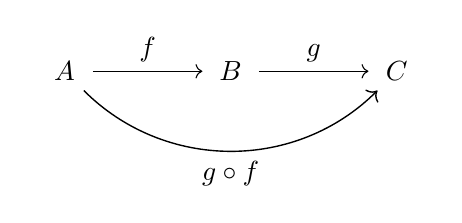
\begin{tikzpicture}
\matrix (m) [matrix of math nodes, row sep=3em, column sep=4em, minimum width=2em]
{
	A & B & C \\
};
\path[->]
(m-1-1) edge node [above] {$f$} (m-1-2)
(m-1-2) edge node [above] {$g$} (m-1-3);
		\path[-{>[scale=1.15]}, line width=0.5pt]
(m-1-1) edge[bend right=45] node [below] {$g\circ f$} (m-1-3);
\end{tikzpicture} \qquad \qquad \, \, \text{ dual :} 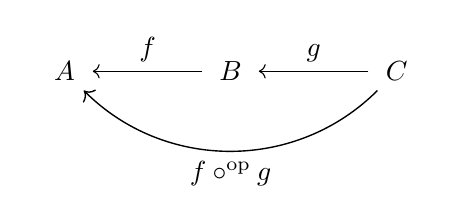
\begin{tikzpicture}
\matrix (m) [matrix of math nodes, row sep=3em, column sep=4em, minimum width=2em]
{
	A & B & C \\
};
\path[->]
(m-1-3) edge node [above] {$g$} (m-1-2)
(m-1-2) edge node [above] {$f$} (m-1-1);
		\path[-{>[scale=1.15]}, line width=0.5pt]
(m-1-3) edge[bend left=45] node [below] {$f\circ^{\text{op}} g$} (m-1-1);
\end{tikzpicture}
\]		
or, equivalently (notation-wise)
\[
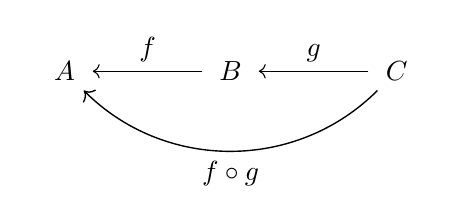
\begin{tikzpicture}
\matrix (m) [matrix of math nodes, row sep=3em, column sep=4em, minimum width=2em]
{
	A & B & C \\
};
\path[->]
(m-1-3) edge node [above] {$g$} (m-1-2)
(m-1-2) edge node [above] {$f$} (m-1-1);
		\path[-{>[scale=1.15]}, line width=0.5pt]
(m-1-3) edge[bend left=45] node [below] {$f \circ g$} (m-1-1);
\end{tikzpicture}
\qquad \qquad \, \, \text{ dual :} 
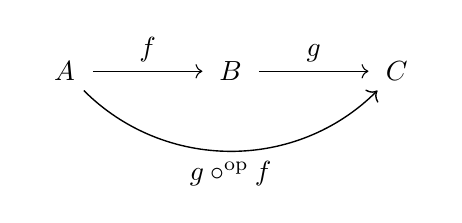
\begin{tikzpicture}
\matrix (m) [matrix of math nodes, row sep=3em, column sep=4em, minimum width=2em]
{
	A & B & C \\
};
\path[->]
(m-1-1) edge node [above] {$f$} (m-1-2)
(m-1-2) edge node [above] {$g$} (m-1-3);
		\path[-{>[scale=1.15]}, line width=0.5pt]
(m-1-1) edge[bend right=45] node [below] {$g\circ^{\text{op}} f$} (m-1-3);
\end{tikzpicture} 
\]		
in that 
\[
\begin{gathered}
g \circ^{\text{op}} f \text{ of } \begin{aligned} & \quad \\
& f \in \text{Hom}_{\mathbf{A}^{\text{op}}}(A,B) \\
& g \in \text{Hom}_{\mathbf{A}^{\text{op}}}(B,C) 
\end{aligned}		 \\
\text{ then } \\
g \circ^{\text{op}} f = f\circ g
\end{gathered}
\]
\end{itemize}
\end{definition}


e.g. if $\mathbf{A} = (M,\cdot, e)$ monoid, then $\mathbf{A}^{\text{op}} = (M, \widehat{\cdot},e)$ where $a\widehat{\cdot} b = b\cdot a$


\subsubsection{Example}

\begin{itemize}
	\item $\text{Vec}^{\text{op}}$
	\[
	\textbf{Vec}^{\text{op}} = (\text{Obj}(\textbf{Vec}), \text{Hom}_{\textbf{Vec}^{\text{op}}}, 1, \circ^{\text{op}})
	\]
	s.t.
	\[
	\text{Hom}_{\textbf{Vec}^{\text{op}} }(W,V) = \text{Hom}_{\textbf{Vec}}(V,W)
	\]
\[	
	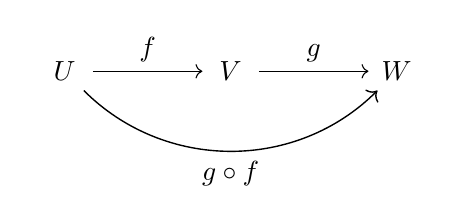
\begin{tikzpicture}
	\matrix (m) [matrix of math nodes, row sep=3em, column sep=4em, minimum width=2em]
	{
		U & V & W \\
	};
	\path[->]
	(m-1-1) edge node [above] {$f$} (m-1-2)
	(m-1-2) edge node [above] {$g$} (m-1-3);
		\path[-{>[scale=1.15]}, line width=0.5pt]
	(m-1-1) edge[bend right=45] node [below] {$g\circ f$} (m-1-3);
	\end{tikzpicture} \qquad \, 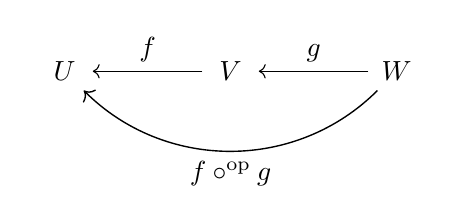
\begin{tikzpicture}
	\matrix (m) [matrix of math nodes, row sep=3em, column sep=4em, minimum width=2em]
	{
		U & V & W \\
	};
	\path[->]
	(m-1-3) edge node [above] {$g$} (m-1-2)
	(m-1-2) edge node [above] {$f$} (m-1-1);
		\path[-{>[scale=1.15]}, line width=0.5pt]
(m-1-3) 	edge[bend left=45] node [below] {$f\circ^{\text{op}} g$} (m-1-1);
	\end{tikzpicture}
\]
\end{itemize}

\subsection{Kinds of morphisms}

\begin{definition}[isomorphism]
	\textbf{isomorphism} - morphism $f:A \to B$ is an isomorphism if $\exists \, g : B \to A$ s.t. $f\circ g = 1_B$, $g\circ f = 1_A$, $g$ unique. $g$ called inverse of $f,f^{-1}$
	\[
	\begin{gathered}
	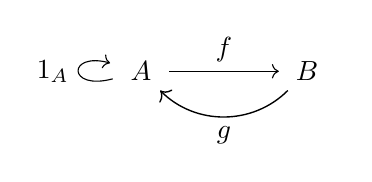
\begin{tikzpicture}
\matrix (m) [matrix of math nodes, row sep=3em, column sep=4em, minimum width=2em]
{
	A & B \\
};
\path[->]
(m-1-1) edge node [above] {$f$} (m-1-2)
		edge [loop left] node [left] {$1_A$} (m-1-1);
		\path[-{>[scale=1.15]}, line width=0.5pt]
(m-1-2) edge[bend left=45] node [below] {$g$} (m-1-1);
\end{tikzpicture}	\qquad \, 
	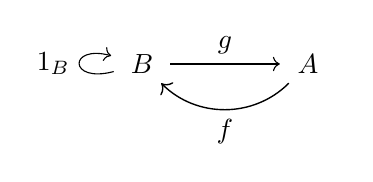
\begin{tikzpicture}
\matrix (m) [matrix of math nodes, row sep=3em, column sep=4em, minimum width=2em]
{
	B & A \\
};
\path[->]
(m-1-1) edge node [above] {$g$} (m-1-2)
		edge [loop left] node [left] {$1_B$} (m-1-1);
\path[-{>[scale=1.15]}, line width=0.5pt]
(m-1-2) edge[bend left=45] node [below] {$f$} (m-1-1);
\end{tikzpicture}	
	\end{gathered}	
	\]
\end{definition}

\begin{definition}[endomorphism]
	\textbf{endomorphism} - morphism with same source and target, that is, morphism $f:A \to A$
\end{definition}

\begin{definition}[automorphism]
\textbf{automorphism} - endomorphism which is an isomorphism
\end{definition}

\begin{definition}[parallel]
	\textbf{parallel} - 2 morphisms $f,g$ are parallel if they have same source and same target:
	\[
	\begin{aligned}
	& f:A \to B \\
	& g:A \to B
	\end{aligned}
	\]
\end{definition}

\begin{definition}[monomorphism]
	\text{monomorphism} - morphism $f: A \to B$ is a monomorphism if $\forall \, $ pair of parallel $\begin{aligned}
	& \quad \\
	& g_1: C \to A \\
	& g_2:C \to A
	\end{aligned}$, 
	\begin{equation}
	f\circ g_1 = f\circ g_2 \text{ implies } g_1 = g_2
	\end{equation}
	i.e.
	\[
	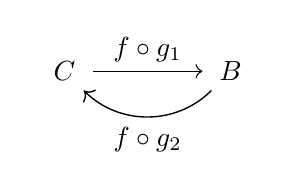
\begin{tikzpicture}
	\matrix (m) [matrix of math nodes, row sep=3em, column sep=4em, minimum width=2em]
	{
		C & B \\
	};
	\path[->]
	(m-1-1) edge node [above] {$f \circ g_1$} (m-1-2);
	\path[-{>[scale=1.15]}, line width=0.5pt]
	(m-1-2) edge[bend left=45] node [below] {$f\circ g_2$} (m-1-1);
	\end{tikzpicture} \text{ implies } C \xrightarrow{ g_1 = g_2 } A	
	\]
\end{definition}

\begin{definition}[epimorphism]
\textbf{epimorphism} - morphism $f:A \to B$ is an epimorphism if $f^{\text{op}} : B^{\text{op}} \to A^{\text{op}}$ is a monomorphism in $\mathbf{A}^{\text{op}}$. \\
Hence $f$ epimorphism iff $\forall \, $ parallel morphisms $\begin{aligned} & \quad \\ 
	& g_1 : B \to C \\
	& g_2 : B\to C\end{aligned}$, $g_1 \circ f = g_2 \circ f $ \\
	 implies $g_1 = g_2$
\end{definition}

\begin{proposition}[monomorphism, epimorphism iff injective]
	$f$ monomorphism iff $f \circ : \text{Hom}_{\mathbf{A}}(C,A) \to \text{Hom}_{\mathbf{A}}(C,B)$ injective \, $\forall \, C \in \text{Obj}(\mathbf{A})$, i.e.
	\begin{equation}
	\begin{gathered}
	\text{Hom}_{\mathbf{A}}(C, A) \xrightarrow{f \circ } \text{Hom}_{\mathbf{A}}(C,B) \\
 g_1 = g_2 \xmapsto{f \circ} f\circ g_1 = f\circ g_2
\end{gathered}
	\end{equation}
$f$ epimorphism iff map $\circ f : \text{Hom}_{\mathbf{A}}(B,C) \to \text{Hom}_{\mathbf{A}}(A,C)$ injective $\forall \, C \in \text{Obj}(\mathbf{A})$
\begin{equation}
\begin{gathered}
\text{Hom}_{\mathbf{A}}(B, C) \xrightarrow{\circ f} \text{Hom}_{\mathbf{A}}(A,C) \\
g_1 = g_2  \xmapsto{ \circ f} g_1\circ f = g_2 \circ f
\end{gathered}
\end{equation}
\end{proposition}

\begin{definition}[inverses]
	$\forall \, $ 2 morphisms, $f:X\to Y$, $g: Y \to X$ s.t. $f\circ g= 1_Y$,\\
	$f$ is called left inverse of $g$, $g$ is called right inverse of $f$.
	
	We also say, $g$ is a section of $f$, or $f$ is a cosection of $g$. \\
	$f$ is an epimorphism, $g$ is a monomorphism.
\end{definition}

\subsection{More definitions with categories}

\begin{definition}[subcategory]
category $\mathbf{A}'$, $\mathbf{A}' \subset \mathbf{A}$, if $\text{Obj}(\mathbf{A}') \subset \text{Obj}(\mathbf{A})$, $\text{Hom}_{\mathbf{A}'}(A,B) \subset \text{Hom}_{\mathbf{A}}(A,B)$, $\forall \, A, B \in \mathbf{A}'$.

Composition in $\mathbf{A}'$ is induced by composition in $\mathbf{A}$.\\
identity morphisms in $\mathbf{A}'$ are identity morphisms in $\mathbf{A}$
\end{definition}

\begin{definition}[full subcategory]
	subcategory $\mathbf{A}'$ of $\mathbf{A}$ is full if $\text{Hom}_{\mathbf{A}'}(A,B) = \text{Hom}_{\mathbf{A}}(A,B)$, $\forall \, A, B \in \mathbf{A}'$	
\end{definition}

\begin{definition}[saturated subcategory]
full subcategory $\mathbf{A}'$ of $\mathbf{A}$ saturated if $A \in \mathbf{A}$ belongs to $\mathbf{A}'$ whenever $A$ is isomorphic to object of $\mathbf{A}'$	
\end{definition}

\begin{definition}[discrete category]
	\textbf{discrete} - discrete category if all morphisms are identity morphisms.
\end{definition}

\begin{definition}[nonempty category]
	\textbf{nonempty} - nonempty category if $\text{Obj}(\mathbf{A})$ is nonempty
\end{definition}

\begin{definition}[groupoid]
\textbf{groupoid} - category $\mathbf{A}$ is a \textbf{groupoid} if all morphisms are isomorphisms.
\end{definition}

\begin{definition}[finite category]
	finite - finite category if set of all morphisms in $\mathbf{A}$ (hence, in particular, set of objects) is a finite set
\end{definition}

\begin{definition}[connected]
	connected category $\mathbf{A}$ if it's nonempty, and $\forall \, A,B \in \text{Obj}\mathbf{A}$, $\exists \, $ finite sequence of objects $(A_0 \dots A_n)$, $A_0 = A$, $A_n = B$, s.t. at least 1 of the sets $\text{Hom}_{\mathbf{A}}(A_j, A_{j+1})$ or $\text{Hom}_{\mathbf{A}}(A_{j+1}, A_j)$ is nonempty $\forall \, j \in \mathbb{N}$, with $0\leq j \leq n-1$
\end{definition}

\begin{definition}[monoid $M$]
	\textbf{monoid} $M$ (set endowed with internal product with associative and unital law) is nothing but a category with only 1 object (to $M$, associate category $\mathbf{M}$, with single object $A$, and morphisms $\text{Hom}_{\mathbf{M}}(A,A) = M$)
\end{definition}
	

\part{Reading notes on Cox, Little, O'Shea's \emph{Ideals, Varieties, and Algorithms: An Introduction to Computational Algebraic Geometry and Commutative Algebra}}

\section{Geometry, Algebra, and Algorithms}

\subsection{Polynomials and Affine Space}

fields are important is that linear algebra works over \emph{any} field

\begin{definition}[2] set of all polynomials in $x_1 , \dots , x_n$ with coefficients in $k$, denoted $k[x_1, \dots , x_n]$

\end{definition}

polynomial $f$ \emph{divides} polynomial $g$ provided $g= fh$ for some $h \in k[x_1, \dots , x_n ]$

$k[x_1, \dots, x_n]$ satisfies all field axioms except for existence of multiplicative inverses; commutative ring, $k[x_1, \dots , x_n]$ \emph{polynomial ring}


\subsubsection*{Exercises for 1 }

\exercisehead{1}
$\mathbb{F}_2$ commutative ring since it's an abelian group under addition, commutative in multiplication, and multiplicative identity exists, namely $1$.  It is a field since for $1\neq 0$, the multiplicative identity is $1$.  

\exercisehead{2}
\begin{enumerate}
\item[(a)]
\item[(b)]
\item[(c)]
\end{enumerate}




\subsection{Affine Varieties }


\subsection{Parametrizations of Affine Varieties}


\subsection{Ideals}



\subsection{Polynomials of One Variable}




\section{Groebner Bases}

\subsection{Introduction}




\subsection{Orderings on the Monomials in $k[x_1, \dots , x_n]$ }




\subsection{A Division Algorithm in $k[x_1, \dots , x_n ]$ }



\subsection{Monomial Ideals and Dickson's Lemma }


\subsection{The Hilbert Basis Theorem and Groebner Bases}


\subsection{Properties of Groebner Bases}



\subsection{Buchberger's Algorithm}






\section{Elimination Theory}



\subsection{The Elimination and Extension Theorems}


\subsection{The Geometry of Elimination}



\section{The Algebra-Geometry Dictionary}


\subsection{Hilbert's Nullstellensatz}


\subsection{Radical Ideals and the Ideal-Variety Correspondence}



\section{Polynomial and Rational Functions on a Variety}


\subsection{Polynomial Mappings }


\section{Robotics and Automatic Geometric Theorem Proving}



\subsection{Geometric Description of Robots}






\part{Reading notes on Cox, Little, O'Shea's \emph{Using Algebraic Geometry}}

\textbf{Using Algebraic Geometry}.  David A. Cox.  John Little. Donal O'Shea. Second Edition.  Springer.  2005.  ISBN 0-387-20706-6 QA564.C6883 2004

\section{ Introduction }

\subsection{ Polynomials and Ideals }

\emph{monomial } 

\begin{equation}
  (1.1) \quad \quad \, x_1^{\alpha_1} \dots x_n^{\alpha_n}
\end{equation}

total degree of $x^{\alpha}$ is $\alpha_1 + \dots + \alpha_n \equiv |\alpha|$ \\



field $k$, $k[x_1 \dots x_n]$ collection of all polynomials in $x_1 \dots x_n$ with coefficients $k$.   \\

polynomials in $k[x_1 \dots x_n]$ can be added and multiplied as usual, so $k[x_1 \dots x_n]$ has structure of commutative ring (with identity) \\
however, only nonzero constant polynomials have multiplicative inverses in $k[x_1 \dots x_n]$, so $k[x_1 \dots x_n]$ not a field \\
\quad however set of rational functions $\lbrace f/g | f,g \in k[x_1 \dots x_n], \, g\neq 0\rbrace$ is a field, denoted $k(x_1 \dots x_n)$ \\

so
\[
f = \sum_{\alpha} c_{\alpha}x^{\alpha}
\]
where $c_{\alpha} \in k$

so

\[
f \in k [x_1 \dots x_n ] = \lbrace f | f = \sum_{\alpha} c_{\alpha} x^{\alpha} , x^{\alpha} = x_1^{\alpha_1} \dots x_n^{\alpha_n}, c_{\alpha} \in k \rbrace
\]

$f$ homogeneous if all monomials have same total degrees

polynomial $f$ is homogeneous if all monomials have the \emph{same total degree} \\

Given a collection of polynomials $f_1 \dots f_s \in k[x_1 \dots x_n]$, we can consider all polynomials which can be built up from these by multiplication by arbitrary polynomials and by taking sums

\begin{definition}[1.3] Let $f_1 \dots f_s \in k[x_1 \dots x_n]$ \\
Let $\langle f_1 \dots f_s \rangle = \lbrace p_1 f_1  + \dots + p_s f_s | p_i \in k[x_1 \dots x_n] \text{ for } i = 1 \dots s \rbrace$
\end{definition}


\exercisehead{1} 
\begin{enumerate}
\item[(a)] $x^2 = x \cdot ( x  -y^2 ) + y \cdot ( xy )$  
\item[(b)] 
\[
 p \cdot ( x - y^2 ) = p x - p y^2
\]
and for $p xy = (py)x$
\item[(c)] 
\[
p(y) ( x - y^2) = p(y)x - p(y) y^2 \notin \langle x^2, xy \rangle
\]
\end{enumerate}

\exercisehead{2} 
\[
\begin{gathered}
  \sum_{i=1}^s p_i f_i  + \sum_{j=1}^s q_j f_j = \sum_{i=1}^s (p_i + q_i )f_i, \quad \, p_i + q_i \in k[x_1 \dots x_n] \end{gathered}
\]
$\langle f_1 \dots f_s \rangle$ closed under sums in $k[x_1 \dots x_n]$ \\

If $f\in \langle f_1 \dots f_s \rangle$, \\
\phantom{If }$ p \in k [x_1 \dots x_n]$

\[
\begin{gathered}
p\cdot f = p \sum_{i=1}^s q_j f_j = \sum_{i=1}^s pq_j f_j, \quad \, pq_j \in k[x_1 \dots x_n] \text{ so }  \\
p\cdot f \in \langle f_1 \dots f_s \rangle
\end{gathered}
\]

Done.  \\

The 2 properties in Ex. 2 are defining properties of ideals in the ring $k[x_1 \dots x_n]$

\begin{definition}[1.5]
Let $I \subset k[x_1 \dots x_n]$, \, $I \neq \emptyset$ \\
$I$ ideal if 
\begin{enumerate}
\item[(a)] $f+ g \in I$, \, $\forall \, f,g \in I$ 
\item[(b)] $pf \in I$, \, $\forall \, f \in I$, arbitrary $p \in k[x_1 \dots x_n]$
\end{enumerate}
\end{definition}

Thus $\langle f_1 \dots f_s\rangle$ is an ideal by Ex. 2.  \\

we call it the ideal generated by $f_1 \dots f_s$.  

\exercisehead{3} Suppose $\exists \, $ ideal $J$, $f_1 \dots f_s \in J$ s.t. $J \subset \langle f_1 \dots f_s \rangle$ \\
if $f\in \langle f_1 \dots f_s \rangle$, $f = \sum_{i=1}^s p_i f_i$, \, $p_i \in k[x_1 \dots x_n]$ \\

$\forall \, i = 1 \dots s$, $p_i f_i \in J$ and so $\sum_{i=1}^s p_i f_i \in J$, by def. of $J$ as an ideal.

\[
\langle f_1 \dots f_s \rangle \subseteq J \quad \quad \, \Longrightarrow J = \langle f_1 \dots f_s \rangle
\]

$\Longrightarrow \langle f_1 \dots f_s \rangle$ is smallest ideal in $k[x_1 \dots x_n]$ containing $f_1 \dots f_s$


\exercisehead{4} For $\begin{aligned} & \quad \\
  & I = \langle f_1 \dots f_s \rangle \\
  & J = \langle g_1 \dots g_t \rangle \end{aligned}$ \\

 $I = J$ iff $s=t$ and $\forall \, f \in I$, $f = \sum_{i=1}^t q_i g_i$ and if $ 0  = \sum_{i=1}^t q_i g_i$, $q_i =0$, \, $\forall \, i = 1 \dots t$, and if $0 = \sum_{i=1}^s p_i f_i$, \, $p_i = 0$, \, $\forall \,  i = 1 \dots s$


\begin{definition}[1.6]
\[
\sqrt{I} = \lbrace g \in k[x_1\dots x_n] | g^m \in I \text{ for some } m \geq 1 \rbrace
\]
\end{definition}

e.g. $x+y \in \sqrt{ \langle x^2 + 3 xy , 3xy + y^2 \rangle }$

in $\mathbb{Q}[x,y]$ since 

\[
(x+y)^3 =x(x^2 + 3xy) + y(3xy + y^2) \in \langle x^2 + 3xy, 3xy + y^2\rangle
\]


%\begin{definition}[1.6]
%\[
%\sqrt{I } = \lbrace g \in k[x_1 \dots x_n ] | g^m \in I \text{ for some m } \geq 1 \rbrace
%\]
%\end{definition}

%e.g. $x+y \in \sqrt{ \langle x^2 + 3xy, 3xy + y^2 \rangle }$

%in $\mathbb{Q}[x,y]$ since

%\[
%(x+y)^3 = x(x^2 + 3xy) + y(3xy + y^2) \in \langle x^2 + 3xy, 3xy + y^2 \rangle
%\]

\begin{itemize}
\item (Radical Ideal Property) $\forall \, $ ideal $I\subset k[x_1 \dots x_n]$, $\sqrt{I}$ ideal, $\sqrt{I} \supset I$
\item \textbf{(Hilbert basis Thm.)} $\forall \, $ ideal $I\subset k[x_1\dots x_n]$ \\
$\exists \, $ finite generating set, \\
i.e. $\exists \, \lbrace f_1 \dots f_2 \rbrace \subset k [x_1 \dots x_n]$ s.t. $I=\langle f_1 \dots f_s \rangle$
\item (Division Algorithm in $k[x]$) $\forall \, f,g \in  k[x]$ (EY : in 1 variable) \\
$\forall \, f, g \in k[x]$ (in 1 variable )\\
$f= qg + r$, $\exists \, !$ quotient $q$, $\exists \, $ remainder $r$
\end{itemize}

\subsection{}

\subsection{Gr\"obner Bases}

\begin{definition}[3.1]
  Gr\"obner basis for $I$ $\equiv G = \lbrace g_1 \dots g_k \rbrace \subset I$ s.t. $\forall \, f \in I$, $\text{LT}(f)$ divisible by $\text{LT}(g_i)$ for some $i$
\end{definition}

\begin{itemize}
\item (Uniqueness of Remainders) let ideal $I\subset k[x_1 \dots x_n]$ \\
division of $f\in k[x_1 \dots x_n]$ by Gr\"o bner basis for $I$, produces $f=g+r$, $g\in I$, and no term in $r$ divisible by any element of $\text{LT}(I)$
\end{itemize}





\subsection{Affine Varieties}

affine $n$-dim. space over $k$ \quad \, $k^n = \lbrace (a_1 \dots a_n ) | a_1 \dots a_n \in k \rbrace$

$\forall \, $ polynomial $f\in k[x_1 \dots x_n ]$, $(a_1 \dots a_n) \in k^n$ \\
\phantom{ \quad } $f: k^n \to k$ \\
\phantom{ \quad } $f(a_1 \dots a_n)$ s.t. $x_i = a_i$ i.e. \\

if $f= \sum_{\alpha} c_{\alpha} x^{\alpha}$ for $c_{\alpha} \in k$, then  \\
\phantom{ \quad } $f(a_1 \dots a_n) =\sum_{\alpha} c_{\alpha}a^{\alpha} \in k$, where $a^{\alpha} = a_1^{\alpha_1} \dots a_n^{\alpha_n}$

\begin{definition}[4.1]
affine variety $\mathbf{V}(f_1 \dots f_s) = \lbrace ( a_1 \dots a_n) | (a_1 \dots a_n) \in k^n, \, f_1(x_1 \dots x_n) = \dots = f_s(x_1 \dots x_n) = 0 \rbrace$ \\
subset $V\subset k^n$ is affine variety if $V = V(f_1 \dots f_s)$ for some $\lbrace f_i \rbrace$, polynomial $f_i \in k[x_1 \dots x_n]$
\end{definition}

\begin{itemize}
  \item (Equal Ideals Have Equal Varieties) If $\langle f_1 \dots f_s \rangle = \langle g_1 \dots g_t \rangle$ in $k[x_1 \dots x_n]$, then $\mathbf{V}(f_1 \dots f_s) = \mathbf{V}(g_1 \dots g_t)$
\end{itemize}

so, recap \\
if $\langle f_1 \dots f_s \rangle = \langle g_1 \dots g_t \rangle $ in $k[x_1 \dots x_n]$, \\
then $V(f_1 \dots f_s) = V(g_1 \dots g_t)$   \\

Recall Hilbert basis Thm. $\forall \, $ ideal $I \subset k[x_1 \dots x_n]$ 
\[
I= \langle f_1 \dots f_s \rangle
\]
$\Longrightarrow $ if $I=J$, then $V(I) = V(J)$

think of $V$ defined by $I$, rather than $f_1 = \dots = f_s =0$

\exercisehead{3}

Recall Def. 1.5 Let $I\subset k[x_1 \dots x_n]$ \\
$I$ ideal if $\begin{aligned} & \quad \\
  & f + g \in I  \quad \, \forall \, f,g \in I \\
  & pf \in I, \quad \, \forall \, f \in I \text{ arbitrary } p \in k[x_1 \dots x_n]
\end{aligned}$

Let $f,g \in I(V)$ 
\[
\begin{gathered}
  (f+g)(a_1 \dots a_n) = f(a_1 \dots a_n) + g(a_1 \dots a_n) = 0 + 0 = 0 \quad \quad \, f+g \in I(V) \\ 
  pf(a_1 \dots a_n) = p(a_1 \dots a_n) f(a_1 \dots a_n) = 0 \quad \quad \, pf \in I(V)
\end{gathered}
\]
Then $I(V)$ an ideal.

%\exercisehead{3} Recall Def. 1.5. Let $I \subset k[x_1 \dots x_n]$, $I$ ideal if $\begin{aligned} & \quad \\
%  & f+g \in I \quad \, \forall \, f,g\in I \\
%  & pf \in I , \quad \, \forall \, f \in I, \text{ arbitrary } p \in k[x_1 \dots x_n ] \end{aligned}$

%Let $f,g \in I(V)$ 
%\[

$V = V(x^2)$ in $\mathbb{R}^2$ \\
$I=\langle x^2 \rangle$ in $\mathbb{R}[x,y]$, \, $I= \lbrace px^2 | p \in k[x,y]\rbrace$ \\
\phantom{ \quad } $I \subset I(V)$, since $px^2 = 0$ for $x^2=0$, $(0,b)$, \, $b\in \mathbb{R}$ \\
But $p(x,y) = x\in I(V)$, as 
\[
I(V) = \lbrace f \in k[x_1 \dots x_n] | f(a_1 \dots a_n)=0, \, \forall \, (a_1\dots a_n) \in V\rbrace
\]
\phantom{ \quad \quad } $p(0,b) = x = 0$

But $x\notin I$

\exercisehead{4} $I\subset \sqrt{I}$

Recall Def. 1.6 $\sqrt{I} = \lbrace g \in k[x_1 \dots x_n] |g^m \in I \text{ for some } m\geq 1\rbrace$ \\
$\forall \, f \in I$, $f=f^1$, $m=1$, so $f\in \sqrt{I}$, \quad \, $I\subset \sqrt{I}$ \\
\phantom{\quad \quad } Hilbert basis thm., $\forall \, $ ideal $I\subset k[x_1 \dots x_n]$ s.t. $I=\langle f_1 \dots f_s \rangle$ \\
\phantom{\quad } $V(I) = \lbrace (a_1 \dots a_n) |(a_1 \dots a_n) \in k^n, \, f_1(a_1\dots a_n) = \dots = f_s(a_1\dots a_n)=0\brace$ \\
$\mathbf{I}(\mathbf{V}(I)) = \lbrace f \in k[x_1 \dots x_n] | f(a_1 \dots a_n) =0 \quad \, \forall \, (a_1 \dots a_n) \in V(I) \rbrace$ \\
Let $g\in \sqrt{I}$, \, $g^m \in I$, \, $g^m=g^{m-1}g$  \\
\phantom{\quad \quad \,} $g^m(a_1 \dots a_n) =0 = g^{m-1}(a_1 \dots a_n)g(a_1 \dots a_n) =0$.  Then $g(a_1 \dots a_n)=0$ or $g^{m-1}(a_1\dots a_m)=0$ \\
\phantom{\quad }as $g^m\in I$, and $V(I)$ is s.t. $f_1(a_1 \dots a_n) = \dots = f_s(a_1 \dots a_n)=0$ for $I=\langle f_1 \dots f_s \rangle$

\begin{itemize}
  \item (Strong Nullstellensatz) if $k$ algebraically closed (e.g. $\mathbb{C}$), $I$ ideal in $k[x_1 \dots x_n]$, then 
\[
\mathbf{I}(\mathbf{V}(I) = \sqrt{I}
\]
\item (Ideal-variety correspondence) Let $k$ arbitrary field
\[
\begin{aligned}
  & I \subset I(V(I)) \\ 
  & V(I(V)) = V \quad \, \forall \, V
\end{aligned}
\]
\end{itemize}

\subsection*{Additional Exercises for Sec.4}

\exercisehead{6}



\section{ Solving Polynomial Equations}

\subsection{}

\subsection{Finite-Dimensional Algebras}

Gr\"obner basis $G = \lbrace g_1 \dots g_t \rbrace$ of ideal $I\subset k[x_1\dots x_n]$, \\
recall def.: Gr\"obner basis $G = \lbrace g_1 \dots g_t\rbrace \subset I$ of ideal $I$, \, $\forall \, f \in I$, $\text{LT}(f)$ divisible by $\text{LT}(g_i)$ for some $i$ \\
\phantom{\quad \, } $f \in k[x_1\dots x_n]$ divide by $G$ produces $f=g+r$, $g\in I$, $r$ not divisible by any $\text{LT}(I)$ uniqueness of $r$ \\
$f\in k[x_1 \dots x_n]$ divide by $G$, 

Recall from Ch. 1, divide $f\in k[x_1 \dots x_n]$ by $G$, the division algorithm yields

\begin{equation}
  (2.1)  \quad \quad \quad \, f = h_1 g_1 + \dots + h_t g_t + \overline{f}^G
\end{equation}
where remainder $\overline{f}^G$ is a linear combination of monomials $x^{\alpha} \notin \langle \text{LT}(I) \rangle $ \\
\phantom{\quad } since Gr\"obner basis, $f\in I$ iff $\overline{f}^G=0$

$\forall \, f \in k[x_1\dots x_n]$, we have coset $[f] = f+I = \lbrace f +h|h\in I\rbrace$ s.t. $[f]=[g]$ iff $f- g \in I$

We have a 1-to-1 correspondence 
\[
\begin{gathered}
\text{remainders } \leftrightarrow \text{ cosets } \\
\overline{f}^G \leftrightarrow [f]
\end{gathered}
\]
algebraic
\[
\begin{aligned}
  & \overline{f}^G + \overline{g}^G \leftrightarrow [f] + [g] \\ 
  & \overline{ \overline{f}^G \cdot \overline{g}^G } \leftrightarrow [f]\cdot [g]
\end{aligned}
\]
$B = \lbrace x^{\alpha} | x^{\alpha} \notin \langle \text{LT}(I) \rangle \rbrace$ is a basis of $A$, basis monomials, standard monomials

20141023 EY's take

$\forall \, [f] \in A = k[x_1 \dots x_n]/I$, \, $[f] = p_ib_i$; \, $b_i \in B = \lbrace x^{\alpha} | x^{\alpha} \notin \langle \text{LT}(I) \rangle \rbrace$ \\
For $I = \langle G \rangle$ \\
\phantom{\quad } e.g. $G=\lbrace x^2 + \frac{3}{2} xy + \frac{1}{2} y^2 - \frac{3}{2} x - \frac{3}{2} y, xy^2-x, y^3-y \rbrace$ \\
$\langle \text{LT}(I) \rangle = \langle x^2, xy^2,y^3 \rangle$ \\
e.g. $B=\lbrace 1,x,y,xy,y^2\rbrace$ \\
\phantom{\quad } $[f]\cdot[g] = [fg]$ \\
e.g. $f=x, \, g=xy, \, [fg] = [x^2y]$ \\
now $f=h_1g_1 + \dots +h_tg_t+ \overline{f}^G$

\subsection{}

\subsection{Solving Equations via Eigenvalues and Eigenvectors}


\section{ Resultants }

\section{Computation in Local Rings}

\subsection{Local Rings}


\begin{definition}[1.1]
  \[
k[x_1 \dots x_n]_{\langle x_1 \dots x_n \rangle} \equiv \lbrace \frac{f}{g} | \text{ rational functions } \frac{f}{g} \text{ of } x_1 \dots x_n \text{ with } g(p) \neq 0 \text{ at } p \rbrace
\]
\end{definition}

main properties of $k[x_1 \dots x_n]_{\langle x_1 \dots x_n \rangle }$

\begin{proposition}[1.2]
  Let $R= k[x_1 \dots x_n]_{\langle x_1 \dots x_n \rangle }$.  Then
\begin{enumerate}
\item[(a)] $R$ subring of field of rational functions $k(x_1 \dots x_n) \supset k[x_1 \dots x_n]$
\item[(b)] Let $M=\langle x_1 \dots x_n \rangle \subset R$ (ideal generated by $x_1 \dots X_n$ in $R$) \\
Then $\forall \, \frac{f}{g} \in R \backslash M$, $\frac{f}{g}$ unit in $R$ (i.e. multiplicative inverse in $R$)
\item[(c)] $M$ maximal ideal in $R$
\end{enumerate}
\end{proposition}


\exercisehead{1} if $p=(a_1 \dots a_n) \in k^n$, $R = \lbrace \frac{f}{g} | f,g\in k[x_1 \dots x_n] , \, g(p) \neq 0 \rbrace$ 
\begin{enumerate}
\item[(a)] $R$ subring of field of rational functions $k(x_1 \dots x_n)$ 
\item[(b)] Let $M$ ideal generated by $x_1 - a_1 \dots x_n -a_n$ in $R$  \\
Then $\forall \, \frac{f}{g} \in R\backslash M$, $\frac{f}{g}$ unit in $R$ (i.e. multiplicative inverse in $R$)
\item[(c)]  $M$ maximal ideal in $R$
\end{enumerate}


\begin{proof}
let $p = (a_1 \dots a_n) \in k^n$ \\
let $g_1(p) \neq 0$, $g_2(p) \neq 0$ 
\[
\begin{gathered}
  \frac{f_1}{g_1 } + \frac{f_2}{g_2} = \frac{f_1 g_2 + f_2 g_1}{ g_1 g_2 } \quad \quad \,  g_1(p)g_2(p) \neq 0 \text{ so } \frac{f_1}{g_1} + \frac{f_2}{g_2} \in R \\
 \frac{f_1}{g_1} \cdot \frac{f_2}{g_2} = \frac{f_1 f_2}{g_1 g_2} \quad \quad \, g_1(p) g_2(p) \neq 0 \text{ so } \frac{f_1}{g_1}\frac{f_2}{g_2} \in R
\end{gathered}
\]
$f= \frac{f}{I} \in R$, \quad \, $\forall \, f\in k[x_1 \dots x_n]$, so $k[x_1 \dots x_n]\subset R$

\end{proof}

EY : 20141027, to recap, 

Let $V = k^n$ \\
Let $p = (a_1 \dots a_n)$ \\
single pt. $\lbrace p \rbrace$ is (an example of) a variety \\
$I(\lbrace p \rbrace) = \lbrace x_1 -a_1 \dots x_n -a_n \rangle \subset k[x_1 \dots x_n]$ \\

$R \equiv k[x_1 \dots x_n]_{\langle x_1 - a_1 \dots x_n-a_n \rangle }$ 
\[
R = \lbrace \frac{f}{g} | \text{ rational function $\frac{f}{g}$ of $x_1 \dots x_n$, $g(p) \neq 0$, $p=(a_1 \dots a_n) $ } \rbrace
\]

Prop. 1.2. properties 

\begin{enumerate}
\item[(a)] $R$ subring of field of rational functions $k(x_1 \dots x_n)$ \quad \, $k(x_1 \dots x_n) \subset R$ 
\item[(b)] $M = \langle x_1 \dots a_1 \dots x_n -a_n \rangle \subset R$.  ideal generated by $x_1 - a_1 \dots x_n-a_n$ \\
Then $\forall \, \frac{f}{g} \in R\backslash M$, $\frac{f}{g}$ unit in $R$ ( $\exists \, $ multiplicative inverse in $R$ )
\item[(c)] $M$ maximal ideal in $R$. \\
in $R$ we allow denominators that are not elements of this ideal $I(\lbrace p \rbrace)$ 
\end{enumerate}

\begin{definition}[1.3] local ring is a ring that has exactly 1 maximal ideal \end{definition}

\begin{proposition}[1.4] ring $R$ with proper ideal $M\subset R$ is local ring if $\forall \, \frac{f}{g} \in R\backslash M$ is unit in $R$
\end{proposition}

localization Ex. 8, Ex. 9 \\
parametrization

\exercisehead{2} \[
\begin{aligned}
  & x = x(t) = \frac{-2t^2 }{1+t^2} \\ 
 &  y = y(t) = \frac{2t}{1+t^2}
\end{aligned}
\]
$k[t]_{\langle t \rangle}$ \quad \, $\frac{-2t^2}{1+t^2}$ rational function of $t$.  $1+t^2 \neq 0$

if $k = \mathbb{C}$ or $\mathbb{R}$ \\

Consider set of convergent power series in $n$ variables \\

\begin{equation}
(1.5) \quad \quad \,   k\lbrace x_1 \dots x_n \rbrace = \lbrace \sum_{\alpha \in \mathbb{Z}^n_{\geq 0}} c_{\alpha} x^{\alpha} | c_{\alpha} \in k, \text{ series converges in some open $U\ni 0 \in k^n $ } \rbrace
\end{equation}

Consider set $k[[x_1 \dots x_n]]$ of formal power series

\begin{equation}
  (1.6) \quad \quad \, k[[x_1 \dots x_n]] = \lbrace \sum_{\alpha \in \mathbb{Z}^n_{\geq 0}} c_{\alpha} x^{\alpha} | c_{\alpha} \in k \rbrace \text{ series need not converge }
\end{equation} 


variety $V$ \\

$k[x_1\dots x_n]/\mathbf{I}(V)$ \phantom{ \quad \quad \quad } variety $V$


\subsection{Multiplicities and Milnor Numbers}


if $I$ ideal in $k[x_1\dots x_n]$, then denote $Ik[x_1\dots x_n]_{\langle x_1 \dots x_n \rangle}$ ideal generated by $I$ in larger ring $k[x_1\dots x_n]_{\langle x_1 \dots x_n \rangle}$

\begin{definition}[2.1] Let $I$ $0$-dim. ideal in $k[x_1 \dots x_n]$, so $V(I)$ consists of finitely many pts. in $k^n$.  \\
Assume $(0 \dots 0) \in V(I)$ \\
multiplicity of $(0\dots 0)\in V(I)$ is 
\[
\text{dim}_k{ k[x_1\dots x_n]_{\langle x_1\dots x_n \rangle}} / Ik[x_!\dots x_n]_{\langle x_1 \dots x_n \rangle}
\]
\end{definition}


generally, if $p=(a_1 \dots a_n) \in V(I)$ \\
multiplicity of $p$, $m(p) = \text{dim}{ k[x_1 \dots x_n]_M } / Ik[x_1 \dots x_n]_M$

\[
\text{dim}{ k[x_1 \dots x_n]_M } / Ik[x_1 \dots x_n]_M
\]

localizing $k[x_1 \dots x_n]$ at maximal ideal $M = I(\lbrace p \rbrace) = \langle x_1 - a_1 \dots x_n-a_n \rangle$


\section{}

\section{}

\section{ Polytopes, Resultants, and Equations }

\section{ Polyhedral Regions and Polynomials }

\subsection{ Integer Programming }

Prop. 1.12. \\

Suppose 2 customers $A, B$ ship to same location \\
\quad A: ship 400 kg pallet taking up $2 \, m^3$ volume \\
\quad B: ship 500 kg pallet taking up $3 \, m^3$ volume \\

shipping firm trucks carry up to 3700 \, kg, up to $20 \, m^3$ \\

B's product more perishable, paying \$ 15 per pallet \\

A pays \$ 11 per pallet

How many pallets from A, B each in truck to maximize revenues?

\begin{equation}
(1.1) \quad \quad \, \begin{gathered}
    4A + 5B \leq 37 \\
    2A  + 3B \leq 20 \\
    A, B \in \mathbb{Z}^*_{ \geq 0 } \end{gathered}
\end{equation}

maximize $11 A + 15 B$ \\

integer programming. \\
max. or min. value of some linear function 

\[
l(A_1 \dots A_n) = \sum_{i=1}^n c_i A_i 
\]

on set $(A_1 \dots A_n) \in \mathbb{Z}^n_{ \geq 0}$ s.t. 


3. Finally, by introducing additional variables; rewrite linear constraint inequalities as equalities. The new variables are called ``slack variables''

\begin{equation}
(1.4) \quad \quad \, a_{ij} A_j = b_i, \quad \, A_j \in \mathbb{Z}_{\geq 0}
\end{equation}

introduce indeterminate $z_i$, \, $\forall \, $ equation in (1.4)

\[
z_i^{a_{ij} A_j} = z_i^{b_i}
\]

$m$ constraints

\[
\prod_{i=1}^m z_i^{a_{ij}A_j} = \prod_{i=1}^m z_i^{b_i} = \left( \prod_{i=1}^m z_i^{a_{ij}} \right)^{ A_j}
\]

\begin{proposition}[1.6]
  Let $k$ field, define $\varphi: k[w_1 \dots w_n] \to k[z_1 \dots z_m]$ by 
\[
\varphi(w_j) = \prod_{i=1}^m z_i^{a_{ij}} \quad \quad \quad \, \forall \, j = 1 \dots n 
\]

and 

\[
\varphi(g(w_1 \dots w_n) ) = g(\varphi(w_1) \dots \varphi(w_n))
\]
$\forall \, $ general polynomial $g\in k[w_1 \dots w_n]$

Then $(A_1 \dots A_n)$ integer pt. in feasible region iff $\varphi: w_1^{A_1} \dots w_n^{A_n} \mapsto z_1^{b_1} \dots z_m^{b_m}$



\end{proposition}

\exercisehead{3}

Now 

\[
\begin{gathered}
\varphi(w_j) = \prod_{i=1}^m z_i^{a_{ij}} \\
z_i^{a_{ij} A_j} = z_i^{b_i}
\end{gathered}
\]

If $(A_1 \dots A_n)$ an integer pt. in feasible region, $a_{ij} A_j = b_i$

\[
\begin{gathered}
z_i^{a_{ij}A_j } = z_i^{b_i} = \prod_{j=1}^n z_i^{a_{ij} A_j} \Longrightarrow \prod_{j=1}^n \prod_{i=1}^m (z_i^{a_{ij} })^{A_j} = \prod_{i=1}^m z_i^{b_i} = \prod_{j=1}^n \varphi(w_j)^{ A_j} = \prod_{j=1}^n \varphi(w_j)^{A_j} = \varphi\left( \prod_{j=1}^n w_j^{ A_j } \right) = \prod_{i=1}^m z_i^{b_i}
\end{gathered}
\]
since $\varphi(g(w_1 \dots w_n)) = g(\varphi(w_1) \dots \varphi(w_n))$ \\

If $\varphi: \prod_{j=1}^n w_j^{A_j} \mapsto \prod_{i=1}^m z_i^{b_i}$

\[
\varphi\left( \prod_{j=1}^n w_j^{A_j} \right) = \prod_{j=1}^n (\varphi(w_j))^{A_j} = \prod_{i=1}^m z_i^{b_i} = \prod_{j=1}^n \left( \prod_{i=1}^m z_i^{a_{ij}} \right)^{ A_j} \Longrightarrow \prod_{j=1}^n z_i^{a_{ij} A_j} = z_i^{b_i}
\]
or $a_{ij}A_j = b_i$.  So $(A_1\dots A_n)$ integer pt.  




\exercisehead{4} 
\[
\prod_{i=1}^m z_i^{b_i} = \prod_{i=1}^m \prod_{j=1}^n z_i^{ a_{ij} A_j } = \prod_{j=1}^n \left( \prod_{i=1}^m z_i^{a_{ij}} \right)^{A_j} = \prod_{j=1}^n \varphi(w_j)^{A_j} = \varphi\left( \prod_{j=1}^n w_j^{A_j} \right)
\]
So if given $(b_1 \dots b_m) \in \mathbb{Z}^m$, and for a given $a_{ij}$, $a_{ij}A_j = b_i$ \\

For $m\leq n$, then $a_{ij}$ is surjective, so $\exists \, A_j$ s.t. $\prod_{i=1}^m z_i^{b_i} = \varphi\left( \prod_{j=1}^n w_j^{A_j} \right)$



\begin{proposition}[1.8]
Suppose $f_1 \dots f_n \in k[z_1 \dots z_m]$ given \\
Fix monomial order in $k[z_1 \dots z_n, w_1 \dots w_n ]$ with elimination property: \\
$\forall \, $ monomial containing 1 of $z_i$ greater than any monomial containing only $w_j$ \\

Let $\mathcal{G}$ Gr\"{o}bner basis for ideal
\[
I = \langle f_1 - w_1 \dots f_n - w_n \rangle \subset k[z_1 \dots z_m, w_1 \dots w_n]
\]
$\forall \, f \in k[z_1 \dots z_m]$, let $\overline{f}^{ \mathcal{G}}$ be remainder on division of $f$ by $\mathcal{G}$ \\
Then
\begin{enumerate}
\item[(a)] polynomial $f$ s.t. $f\in k[f_1 \dots f_n]$ iff $g= \overline{f}^{ \mathcal{G}} \in k[w_1 \dots w_n]$
\item[(b)] if $\begin{aligned} & \quad \\
  & f \in k [f_1 \dots f_n ] \\
  & g = \overline{f}^{\mathcal{G}}\in k[ w_1 \dots w_n] \end{aligned}$ \quad as in part (a), \\

then $f = g(f_1 \dots f_n)$ , giving an expression for $f$ as polynomial in $f_j$
\item[(c)] if $\forall \, f_i, f$ monomials, $f\in k[f_1 \dots f_n]$, \\
then $g$ also a monomial.  
\end{enumerate}
\end{proposition}



\subsection{Integer Programming and Combinatorics}



\section{Algebraic Coding Theory}


\section{The Berlekamp-Massey-Sakata Decoding Algorithm}





\href{https://martinralbrecht.files.wordpress.com/2010/07/20131022_buchberger_dtu.pdf}{Gr\"{o}bner Bases, Martin R. Albrecht of the DTU Crypto Group}

\part{Statistical Mechanics: Ising Model}  

\section{Ising Model}  

\subsection{Definition of Ising Model}  

cf. \href{https://en.wikipedia.org/wiki/Ising_model}{Wikipedia, "Ising model"}

Consider set of lattice sites $\Lambda$, each with set of adjacent sites (e.g. \textbf{graph}) forming $d$-dim. lattice.  \\
$\forall \, $ lattice site $k\in \Lambda$, $\exists \, $ discrete variable $\sigma_k$, s.t. $\sigma_k \in \lbrace -1, 1\rbrace$.  \\
spin configuration $\equiv \sigma = (\sigma_k)_{k\in \Lambda}$ is an assignment of spin value to each lattice site.  

i.e. 

$d=1$, consider "line" configuration: $i \in \mathbb{Z}$, $i=0,1,\dots L-1$.  Lattice site $k \in \Lambda = \Lambda_{d=1}$.  $\forall \, k \in \Lambda$, \\ 
$\exists \, $ bijection to its index $i$, $k\mapsto i$, and $\exists \, \sigma_k$ i.e. 
\[
\begin{aligned}
	& \sigma : \Lambda \leftrightarrow \sigma: \mathbb{Z} \to \mathbb{Z}_2 \\ 
	& \sigma(k) \equiv \sigma_k \leftrightarrow \sigma(i) \equiv \sigma_i \mapsto \lbrace -1, 1 \rbrace
\end{aligned}
\]
spin configuration $\sigma : \Lambda \mapsto (\sigma_k)_{k\in \Lambda} \in \lbrace -1,1 \rbrace^{| \Lambda |}$, where $|\Lambda | =L$.  \\
$\forall \, k \in \Lambda$, $\exists \, ! $ only at most 2 edges, given, for $k\mapsto i$, $i+1,i-1$, $\forall \, i = 1 \dots L-2$.  

$d=2$, "rectangle" configuration.  $(i,j) \in \mathbb{Z}^2$.   $\begin{aligned} & \quad \\ 
&	 i \in 0,1,\dots L_x-1 \\ 
&	 j \in 0,1,\dots L_y-1 \end{aligned}$.  Lattice site $\mathbf{k} \in \Lambda = \Lambda_{d=2}$.  \\ $\forall \, \mathbf{k} \in \Lambda$, $\exists \, $ bijection to its "grid coordinates" $(i,j)$, $\mathbf{k} \mapsto (i,j)$, and $\exists \, \sigma_{\mathbf{k}} $ i.e. $\sigma_{\mathbf{k}} = \sigma_{ij} \in \lbrace -1,1\rbrace$.  \\
spin configuration $\sigma: \Lambda \mapsto (\sigma_{\mathbf{k}})_{\mathbf{k} \in \Lambda} \in \lbrace -1,1\rbrace^{|\Lambda|}$, where $|\Lambda | \equiv |\Lambda_{d=2} | = L_xL_y$.  \\
$\forall \, \mathbf{k} \in \Lambda$, $\exists \, !$ only at most 4 edges, given by $\mathbf{k} \mapsto (i,j)$, $(i \pm 1, j ), (i,j\pm 1)$, \  $\begin{aligned} & \quad \\ & i = 1\dots L_x -2 \\ & j = 1\dots L_y-2 \end{aligned}$.  

Note that in both cases, I haven't yet defined the boundary conditions, and leave that to be discussed thoroughly in the future (i.e. following sections).  

There are $2^{|\Lambda|}$ number of configurations in any dim. $d$.  

cf. \href{https://en.wikipedia.org/wiki/Ising_model}{Wikipedia, "Ising model"}

\subsubsection{Interaction $J_{ij} \equiv J_{\mathbf{k} \mathbf{l}}$, Hamiltonian (energy functional)for a configuration $H(\sigma)$}  

$\forall \, $ 2 adjacent (lattice) sites, $i,j \equiv \mathbf{k}, \mathbf{l} \in \Lambda$, let there be an interaction $J_{ij} \equiv J_{\mathbf{k} \mathbf{l}}$ i.e. $\begin{aligned} & \quad \\ 
& J : \Lambda^2 \to \mathbb{R} \\ 
& J: (\mathbf{k}, \mathbf{l}) \mapsto J_{\mathbf{k} \mathbf{l}} \end{aligned}$.   \\
Adjacent means $\exists \, $ edge $\mathbf{k} \mapsto \mathbf{l}$ (the mapping is the edge)  

Suppose $\forall \, $ site $j \equiv \mathbf{l} \in \Lambda$ , $\exists \, $ external magnetic field $h_j \equiv h_{\mathbf{l}}$ interacting with it.  \\
Given (site) configuration $\sigma : \Lambda \mapsto (\sigma_{\mathbf{k}})_{\mathbf{k} \in \Lambda} \in \lbrace -1 ,1 \rbrace^{ | \Lambda | }$.  
\begin{equation}
H(\sigma) = -\sum_{ \langle i j \rangle } J_{ij} \sigma_i \sigma_j - \mu \sum_j h_j \sigma_j \equiv H(\sigma(\Lambda)) = -\sum_{\langle \mathbf{k} \mathbf{l} \rangle } J_{\mathbf{k} \mathbf{l} }\sigma_{\mathbf{k}} \sigma_{\mathbf{l}} - \mu \sum_{ \mathbf{k} \in \Lambda } h_{\mathbf{k}} \sigma_{ \mathbf{k}}
\end{equation}
where $\sum_{ \langle \mathbf{k} \mathbf{l} \rangle }$ is overall pairs of adjacent spins (every pair is counted once),  \\
\phantom{where } $\langle \mathbf{k}, \mathbf{l} \rangle \equiv $ sites $\mathbf{k}, \mathbf{l}$ are nearest neighbors.  

Note sign in 2nd. term, $-\mu \sum_{\mathbf{k}} h_{\mathbf{k}} \sigma_{\mathbf{k}}$ should be positive because of electron's magnetic moment is antiparallel to its spin, but negative term used conventionally.  

Nothing was said about boundary conditions, I propose that it can be either fixed in the summation or by setting $J_{\mathbf{k} \mathbf{l}}=0$.  

$\forall \, \mathbf{k} \in \Lambda$, let $\begin{aligned} & \quad \\
	& \mathbf{y} : \Lambda \to E \\ 
		& \mathbf{y}: \mathbf{k} \mapsto \lbrace \langle \mathbf{k}, \mathbf{l} \rangle_{\mathbf{l}} \end{aligned}$, with $\lbrace \langle \mathbf{k}, \mathbf{l} \rangle \rbrace_{\mathbf{l}}$ be set of all edges from $\mathbf{k}$
		
		Then clearly $\sum_{\langle \mathbf{k} \mathbf{l} \rangle } = \frac{1}{2} \sum_{\mathbf{k} \in \Lambda} \sum_{ \lbrace \langle \mathbf{k} \mathbf{l} \rangle \rbrace_{\mathbf{l}}}$.  
		
		
Taking into account only interaction between adjoining dipoles, on a square lattice: 
\[
E(\sigma) = -J \sum_{k,l=0}^{L-1} ( \sigma_{kl}\sigma_{k,l+1} + \sigma_{kl} \sigma_{k+1, l} )
\]
cf. Landau and Lifshitz \cite{LaLi1980}


EY : 20171223 Things to check from Hjorth-Jensen (2015) \cite{Hjor2015}:  

2-dim. Ising model, with $\mathcal{B} \equiv h_j =0$, undergoes phase transition of 2nd. order: meaning below given critical temperature $T_C$, there's spontaneous magnetization with $\langle \mathcal{M} \rangle \equiv \langle \mathbf{M} \rangle \neq 0$.  $\langle \mathbf{B} \rangle \to 0$ at $T_C$ with \emph{infinite} slope, a behavior called \emph{critical phenomena}.  Critical phenomenon normally marked by 1 or more thermodynamical variables which is 0 above a critical point.  In this case, $\langle \mathbf{B} \rangle \neq 0$, such a parameter normally called \emph{order parameter}.  

Critical phenomena; we still don't have a satisfactory understanding of system's properties close to the critical point, even for simplest 3-dim. systems.  Even mean-field models can predict wrong physics; mean-field theory results in a 2nd.-order phase transition for 1-dim. Ising model, wherea 1-dim. Ising model doesn't predict any spontaneous magnetization at any finite temperature $T$.  

e.g. Consider 1-dim. $N$-spin system.  Assume periodic boundary conditions.  Consider state of all spins up, with total energy $-NJ$ and magnetization $N$.  Flip half of spins (e.g. all spins of index $i>N/2$) so 1st half of spins point upwards and last half points downwards.  Energy is $-NJ + 4J$, net magnetization $0$.  This is an example of a possible disordered state with net magnetization $0$.  Change in energy is too small to stabilize disordered state (to $-NJ$).  

\begin{definition}[configuration probability]
\textbf{configuration probability} $P_{\beta}(\sigma)$ given by Boltzmann distribution:  
\begin{equation}\label{Eq:Isingconfigprob}
 P_{\beta}(\sigma) = \frac{ \exp{ (-\beta H(\sigma))} }{ Z_{\beta} } = \text{ prob. of configuration } \sigma \equiv \sigma(\Lambda) \equiv (\sigma_{\mathbf{k}})_{\mathbf{k} \in \Lambda}
\end{equation} with the partition function as normalization constant $Z_{\beta}$: 
\begin{equation}\label{Eq:IsingPartitionFuncZ}
Z_{\beta} = \sum_{\sigma} \exp{ -\beta H(\sigma)}
\end{equation}
\end{definition}  



cf. pp. 504 Sec. 151 Phase transitions of the second kind in a 2-dim. lattice,  Landau and Lifshitz \cite{LaLi1980}


\begin{equation}\label{Eq:2dIsingZexact}
Z = 2^N(1-x^2)^{-N} \coprod_{p,q=0}^{L-1} \left[ (1+x^2)^2 - 2x(1-x^2) \left( \cos{ \frac{2\pi p}{L} } + \cos{ \frac{2\pi q }{L} } \right) \right]^{1/2} 
\end{equation}
cf. (151.11) of Landau and Lifshitz \cite{LaLi1980}, where $x= \tanh{\theta}$, $\theta = J/T \equiv J/\tau = \beta J$.  

\begin{equation}
\begin{gathered}
\Phi \equiv F = -\tau \ln{Z} = \\
= -\tau N \ln{2} + \tau N \ln{ (1-x^2)} - \frac{\tau}{2} \sum_{p,q=0}^L \ln{ \left[ (1+x^2)^2 - 2x(1-x^2) \left( \cos{ \frac{2\pi p}{L} } + \cos{ \frac{2\pi q }{L} } \right) \right] }
\end{gathered}
\end{equation}

Let $\begin{aligned}& \quad \\ 
& \omega_1 = \frac{2\pi p }{ L } \text{ with } p\to 0 \text{ as } L \to \infty \\ 
& \omega_2 = \frac{2\pi q }{ L } \text{ with } q\to 0 \text{ as } L \to \infty \end{aligned}$ so $\begin{aligned} & \quad \\ 
& \frac{ L d\omega_1 }{2\pi } = dp \\ 
& \frac{ L d\omega_2}{ 2\pi } = dq \end{aligned}$ and using $L^2 = N$.  


\[
\Phi = -\tau N \ln{2} + \tau N \ln{ (1-x^2)} - \frac{N\tau }{ 2(2\pi)^2 } \int_0^{2\pi } \int_0^{2\pi } d\omega_1 d\omega_2 \ln{ \left[ (1-x^2) -  2x(1-x^2) \left( \cos{  \omega_1 } + \cos{  \omega_2 } \right) \right]  }
\] 

$F \equiv \Phi$ has singularity when $  (1-x^2) -  2x(1-x^2) \left( \cos{  \omega_1 } + \cos{  \omega_2 } \right)  $ in $\ln{ \left[ (1-x^2) -  2x(1-x^2) \left( \cos{  \omega_1 } + \cos{  \omega_2 } \right) \right]  }$.  \\
$  (1-x^2) -  2x(1-x^2) \left( \cos{  \omega_1 } + \cos{  \omega_2 } \right) $ minimized when $\cos{\omega_1} = \cos{\omega_2}=1$ (since $-1 < x < 1$) 
\[
\begin{gathered}
\Longrightarrow (1+x^2)^2 - 4x(1-x^2 ) = 1+2x^2 + x^4 - 4x + 4x^3 = (x^2+2x-1)^2 =0 \Longrightarrow x = \frac{-2 \pm \sqrt{ 4-4(-1) } }{2} = -1 + \sqrt{2} \\
x = \tanh{\theta} = \frac{e^{\theta} - e^{-\theta} }{ e^{\theta} + e^{-\theta} } = \sqrt{2}  -1 \text{ or } \begin{gathered}
\qquad \\ e^{\theta} - e^{-\theta} = \sqrt{2} e^{\theta} + \sqrt{2} e^{-\theta} - e^{\theta} - e^{-\theta} \text{ so } \\ 
(2-\sqrt{2}) e^{\theta} = \sqrt{2} e^{-\theta} \\
e^{2\theta} = \frac{\sqrt{2}}{ 2-\sqrt{2}} \left( \frac{2+\sqrt{2} }{ 2 + \sqrt{2}} \right) \text{ or } \\ 
2\theta = \ln{ (1+ \sqrt{2})}
\end{gathered}
\end{gathered}
\]

\[
\begin{gathered}
\frac{J}{T_c} = \frac{1}{2} \ln{ (1+\sqrt{2})} \text{ or } 
\end{gathered}
\]
\begin{equation}
\boxed{ \tau_c = \frac{2J}{ \ln{ (1+\sqrt{2}) }} }
\end{equation}
so that $\tau_C \equiv T_C$ is where phase transition occurs.  

Let $t:= \tau - \tau_c$.  $\theta = \frac{J}{\tau} = \frac{J}{t+\tau_C}$  

Expand about minimum  

EY:20171230 do this explicitly 

\[
\begin{gathered}
\int_0^{2\pi } \int_0^{2\pi} d\omega_1 d\omega_2 \ln{ [ c_1 t^2 + c_2(\omega_1^2 + \omega_2^2 )]} \\ 
F  \equiv \Phi \simeq a + \frac{1}{2} b (\tau-\tau_c)^2 \ln{ |\tau-\tau_c|} \\ 
C = \frac{ \partial^2 F}{ \partial \tau } \simeq - b\tau_c \ln{ |\tau-\tau_c| }
\end{gathered}
\]
with $C$ being heat capacity.  

Order parameter $\langle M \rangle \equiv \eta = \text{constant}(\tau_c - \tau)^{1/8} = \begin{cases} 0 & \text{ if } \tau > \tau_c \\ 
\text{ constant } (\tau_c-\tau)^{1/8} & \text{ if } \tau < \tau_c \end{cases}$  

cf. pp. 505 Sec. 151 Phase transitions of the second kind in a 2-dim. lattice,  Landau and Lifshitz \cite{LaLi1980}, L.Onsager 1947.  

\subsection{An actual calculation of a small number of spins with Ising model}  

Sec. 3.7 "An actual calculation" on pp. 76 of Newman and Barkema (1999) \cite{NeBa1999}
goes through a simple actual Monte Carlo calculation as a test case check so to compare this exact calculation/solution to the simulation, as a test of whether the simulation/program is correct.  This is done in Sec. 1.3 of Newman and Barkema (1999) \cite{NeBa1999}.  

However, none of these promised simple calculations were shown explicitly in Newman and Barkema (1999) \cite{NeBa1999}.  I will forego this simple case.  

\subsection{Explicit calculation showing stencil operation on each spin on a periodic lattice grid}  

Consider 
\[
\begin{gathered}
H(\sigma) = -\sum_{ \langle \mathbf{k} \mathbf{l} \rangle } J \sigma_{\mathbf{k}} \sigma_{\mathbf{l}} =  -J \sum_{i=0}^{L_x-1} \sum_{j=0}^{L_y-1} \sigma_{ij}( \sigma_{i+1j} + \sigma_{ij+1} ) = \\	
= \frac{-J}{2} \left( \sum_{i=0}^{L_x-1} \sum_{j=0}^{L_y-1} \sigma_{ij} (\sigma_{i+1 j} + \sigma_{ij+1} ) + \sum_{i=1}^{L_x} \sum_{j=0}^{L_y-1}   \sigma_{i-1j} (\sigma_{ij} + \sigma_{i-1 j+1} ) \right) = \\
	= \frac{-J}{2} \left( \sum_{i=0}^{L_x-1} \sum_{j=0}^{L_y-1} \sigma_{ij} (\sigma_{i+1 j} + \sigma_{ij+1} ) + \sum_{i=1}^{L_x} \sum_{j=0}^{L_y-1}   \sigma_{i-1j} \sigma_{ij} + \sum_{i=0}^{L_x-1} \sum_{j=1}^{L_y} \sigma_{i j-1} \sigma_{ij} \right) 
\end{gathered}
\]
Now for each of these terms, 
\[
\begin{gathered}
	\sum_{i=1}^{L_x} \sum_{j=0}^{L_y-1} \sigma_{i-1 j} \sigma_{ij} = \sum_{i=1}^{L_x} \left( \sum_{j=1}^{ L_y-1 } \sigma_{i-1 j} \sigma_{ij} + \sigma_{i-1 0 }\sigma_{i0} \right) = \sum_{i=1}^{L_x-1} \left( \sum_{j=1}^{L_y-1} \sigma_{i-1 j} \sigma_{ij} + \sigma_{i-10} \sigma_{i0} \right) + \left( \sum_{j=1}^{L_y-1} \sigma_{L_x-1 j } \sigma_{L_xj} \right) + \sigma_{L_x-1 0 } \sigma_{L_x0}   \\ 
\sum_{i=0}^{L_x-1} \sum_{j=1}^{L_y} \sigma_{ij-1} \sigma_{ij} = \sum_{j=1}^{L_y-1} \left( \sum_{i=1}^{L_x-1} \sigma_{ij-1} \sigma_{ij}+ \sigma_{0j-1} \sigma_{0j} \right)  + \sum_{i=1}^{L_x-1} \sigma_{i L_y-1} \sigma_{iL_y} + \sigma_{0L_y-1} \sigma_{0L_y} 
\end{gathered}
\]
\[
\begin{gathered}
	\sum_{i=0}^{L_x-1} \sum_{j=0}^{L_y-1} \sigma_{ij} (\sigma_{i+1j } + \sigma_{ij+1} ) = \sum_{i=0}^{L_x-1} \left( \sum_{j=1}^{L_y} \sigma_{ij} ( \sigma_{i+1j } + \sigma_{ij+1} ) + \sigma_{i0} (\sigma_{i+1 0 } + \sigma_{i1} ) \right) = \\
	\sum_{i=1}^{L_x-1} \left( \sum_{j=1}^{L_y-1} \sigma_{ij} (\sigma_{i+1j}  + \sigma_{ij+1}) + \sigma_{i0} (\sigma_{i+1 0 } + \sigma_{i1}) \right) + \sum_{j=1}^{L_y-1} \sigma_{0j} (\sigma_{1j} + \sigma_{0j+1} ) + \sigma_{00} (\sigma_{10} + \sigma_{01} )
\end{gathered}
\]

Apply periodic boundary conditions.  Adding up all the terms above, clearly we obtain 1 term which shows the stencil operation for spins on the "interior" of the grid: 
\[
\sum_{i=1}^{L_x-1} \sum_{j=1}^{L_y-1} \sigma_{ij} ( \sigma_{i+1j} + \sigma_{ij+1} + \sigma_{i-1j} + \sigma_{ij-1} )
\]
and if we apply \emph{periodic} boundary conditions, neatly, we'll see all the lattice sites at the boundary also will have this stencil operation:  
\[
\begin{gathered}
	\sum_{i=1}^{L_x - 1} \sigma_{i0} (\sigma_{i+10} + \sigma_{i1} ) + \sum_{j=1}^{L_y-1} \sigma_{0j} (\sigma_{1j} + \sigma_{0j+1} ) + \sigma_{00} (\sigma_{10} + \sigma_{01} ) + \left( \sum_{i=1}^{L_x-1} \sigma_{iL_y-1} \sigma_{i0} \right) + \sigma_{0L_y-1} \sigma_{00} + \sum_{j=1}^{L_y-1} \sigma_{0j-1} \sigma_{0j} +  \\
	+ \sum_{j=1}^{L_y - 1} \sigma_{L_x- 1 j} \sigma_{0j} + \sigma_{L_x-1 0} \sigma_{00} + \sum_{i=1}^{L_x-1} \sigma_{i-10} \sigma_{i0} 
\end{gathered}
\]

Now, we can obtain the following for Hamiltonian, given spin configuration $\sigma$ with a lattice grid obeying periodic conditions:  

\begin{equation}
\begin{gathered}
H(\sigma) = -\frac{J}{2} \sum_{i=0}^{L_x-1} \sum_{j=0}^{L_y-1} \sigma_{ij} (\sigma_{i+1j } + \sigma{i-1j} + \sigma_{ij+1} + \sigma_{ij-1} ) = \\
= \frac{-J}{2} \left[  \sum_{i=0}^{L_x-1} \left( \sum_{ \substack{ j=0 \\ j \neq j' \\ } }^{L_y -1} \sigma_{ij} ( \sigma_{i+1j} +  \sigma_{i-1j} + \sigma_{ij+1} + \sigma_{ij-1} ) + \sigma_{ij'} ( \sigma_{i+1j'} + \sigma_{i-1j'} + \sigma_{ij'+1} + \sigma_{ij'-1}  ) \right)  + \right. \\ 
\left. \sum_{ \substack{j=0 \\ j\neq j' \\ } }^{L_y-1} \sigma_{i'j} ( \sigma_{i'+1j} + \sigma_{i'-1j} + \sigma_{i'j+1} + \sigma_{i'j-1} ) + \sigma_{i'j'} ( \sigma_{i'+1j'}  + \sigma_{i'-1j'} + \sigma_{i'j'+1} + \sigma_{i'j'-1}) \right] 
 \end{gathered}
\end{equation}

Consider a psin flip of $\sigma_{i'j'}$.  Contribution to $\Delta H$ at stencil operation on $\sigma_{i'j'}$, at $(i'j') \in \Lambda$, is 
\[
\frac{-J}{2} ( - \sigma_{i'j'} - \sigma_{i'j'} ) (\sigma_{i'+1j'} + \sigma_{i'-1j'} + \sigma_{i'j'+1} + \sigma_{i'j'-1}) = J\sigma_{i'j'} ( \sigma_{i'+1j'} + \sigma_{i'-1j'} + \sigma_{i'j'+1} + \sigma_{i'j'-1})
\]
Consider $\sigma_{i'j'} \sigma_{i'+1j'}$.  Clearly, term $\sigma_{i-1j'} \sigma_{ij'}$ with $i=i'+1$ only occurs once more in the summation.  Thus, we can definitely conclude that for $\Delta H \equiv \Delta H(\Delta \sigma_{i'j'})$ due to a single spin-flip is 
\begin{equation}
\Delta H(\Delta \sigma_{i'j'}) = 2J\sigma_{i'j'} ( \sigma_{i'+1j'} + \sigma_{i'-1j'} + \sigma_{i'j'+1} + \sigma_{i'j'-1} )
\end{equation}


\url{https://www.colorado.edu/physics/phys7240/phys7240_fa12/notes/Week3.pdf}
\href{https://www.colorado.edu/physics/phys7240/phys7240_fa12/notes/Week3.pdf}{Victor Gurarie, Advanced Statistical Mechanics, Fall 2012}
Exact solution by transfer matrices for 2-dim. Ising model.  


\part{Conformal Field Theory; Virasoro Algebra}  

cf.  Schottenloher (2008)  \cite{Scho2008}

\section{Conformal Transformations}

\begin{definition}[Conformal transformation or conformal map]
Let 2 semi-Riemannian manifolds$(M,g)$, $(M',g')$, $\text{dim}M = \text{dim}M'$, let open $U\subset M$, open $V\subset M'$.  

\textbf{conformal transformation} or \textbf{conformal map} is a smooth $\varphi : U\to V$ of maximal rank, if $\exists \, $ smooth $\Omega : U\to \mathbb{R}^+$ s.t. 
\begin{equation}
	\varphi^* g' = \Omega^2 g
\end{equation}
where $\varphi* g'(X,Y) :=g'(T\varphi(X), T\varphi(Y))$ and $T\varphi: TU \to TV$ denote tangent map (derivative) of $\varphi$.  

$\Omega \equiv $ \emph{conformal factor} of $\varphi$.  
\end{definition}

Locally, $y^i = \varphi^i(x)$, \[
\begin{gathered}
	\frac{ \partial \varphi^i }{ \partial x^j} = \frac{ \partial y^i }{ \partial x^j}
\end{gathered}	
\]
Then
\[
X = X^k \frac{ \partial }{ \partial x^k} = X^k \frac{ \partial y^i }{ \partial x^k} \frac{ \partial }{ \partial y^i } = X^k \frac{ \partial \varphi^i }{ \partial x^k} \frac{ \partial }{ \partial y^k} \in TM
\]
and so 
\[
\begin{gathered}
	\varphi^* g'(X,Y) = g'(T\varphi(X), T\varphi(Y)) = (g')_{ij} X^k \frac{ \partial y^i }{ \partial x^k} Y^l \frac{ \partial y^j }{ \partial x^l} = (g')_{ij} X^k \frac{ \partial \varphi^i }{ \partial x^k } Y^l \frac{ \partial y^j}{ \partial x^l} \\ 
\Longrightarrow (\varphi^* g')_{kl} = (g')_{ij} \frac{ \partial y^i }{ \partial x^k } \frac{ \partial y^j}{ \partial x^l } \\ 
\Longrightarrow (\varphi^* g')_{kl} = (g')_{ij} \frac{ \partial \varphi^i }{ \partial x^k} \frac{ \partial \varphi^j}{ \partial x^l} = \Omega^2 g_{kl}
\end{gathered}
\]


% 20170926  

\begin{definition}
	\textbf{extension} of $G$ by group $A$ is (given by) an \emph{exact sequence} of group homomorphisms.  
	\begin{tikzpicture}
	%\matrix(m)[matrix of math nodes, row sep=3em, column sep=3em, text height=1.5ex, text depth=0.25ex]
	\matrix(m)[matrix of math nodes, row sep=4em, column sep=4em]
	{
		1   &  A & E & G & 1 \\
	};
	%\path[->,font=\scriptsize]
	\path[->]
	(m-1-1) edge node[auto]{$$} (m-1-2)
	(m-1-2) edge node[auto]{$i$} (m-1-3)
	(m-1-3) edge node[auto]{$\pi$} (m-1-4)
	(m-1-4) edge node[auto]{$$} (m-1-5)	
	;
	\end{tikzpicture} 
\end{definition}
cf. Def. 3.1 of Schottenloher (2008)  \cite{Scho2008}.  

Recall that an exact sequence, if $\begin{aligned} & \quad \\
	& \text{im}(1\to A) = \text{ker}(i) \\
	& \text{im}(i) = \text{ker}(\pi) \\
	& \text{im}(\pi) = \text{ker}(G\to 1)
\end{aligned}$

By Thm., 
$1\to A \xrightarrow{i} E$ exact so $i$ injective.  \\
$E\xrightarrow{\pi} G \to 1$ exact so $\pi$ surjective.  

Extension is called \textbf{central} if $A$ abelian and image $\text{im}i$ is in center of $E$, i.e. 
$a\in A, b\in E \Longrightarrow i(a) b = bi(a)$.  

\subsubsection{Examples of extensions of $G$, and central extensions of $G$ (which has a particular $E$)}
\begin{itemize}
\item e.g. central extension has form 
\[
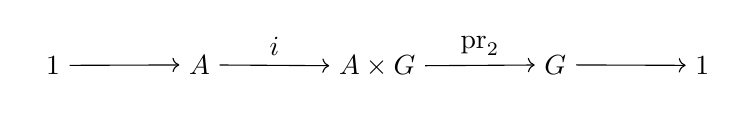
\begin{tikzpicture}
%\matrix(m)[matrix of math nodes, row sep=3em, column sep=3em, text height=1.5ex, text depth=0.25ex]
\matrix(m)[matrix of math nodes, row sep=4em, column sep=4em]
{
	1   &  A & A\times G & G & 1 \\
};
%\path[->,font=\scriptsize]
\path[->]
(m-1-1) edge node[auto]{$$} (m-1-2)
(m-1-2) edge node[auto]{$i$} (m-1-3)
(m-1-3) edge node[auto]{$\text{pr}_2$} (m-1-4)
(m-1-4) edge node[auto]{$$} (m-1-5)	
;
\end{tikzpicture} 
\]
where  \\
$\begin{aligned}
 i:A & \to A\times G \\
a & \mapsto (a,1) \end{aligned}$ 

\[
\begin{gathered}
i(a)(a',g) = (a,1)(a',g) = (aa',g) = \\
= (a'a,g\cdot 1) = (a',g)(a,1) = (a',g)i(a)
\end{gathered}
\]

Notice that what the \emph{exactness} property of an exact sequence does:
\[
\text{pr}_2i(a) = \text{pr}_2(a,1) = 1
\]

\item e.g. of a \text{nontrivial central extension} is exact sequence 
\begin{equation}
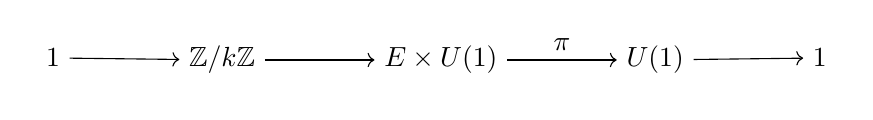
\begin{tikzpicture}
%\matrix(m)[matrix of math nodes, row sep=3em, column sep=3em, text height=1.5ex, text depth=0.25ex]
\matrix(m)[matrix of math nodes, row sep=4em, column sep=4em]
{
	1   &  \mathbb{Z}/k\mathbb{Z} & E\times U(1) & U(1) & 1 \\
};
%\path[->,font=\scriptsize]
\path[->]
(m-1-1) edge node[auto]{$$} (m-1-2)
(m-1-2) edge node[auto]{$$} (m-1-3)
(m-1-3) edge node[auto]{$\pi$} (m-1-4)
(m-1-4) edge node[auto]{$$} (m-1-5)	
;
\end{tikzpicture} 
\end{equation}
with $\pi(z) = z^k$ \, $\forall \, k \in \mathbb{N}$, $k\geq 2$, since $E=U(1)$ and $\mathbb{Z}/k\mathbb{Z}$ are not isomorphic.  

Also, homomorphism $\tau:U(1) \to E$ with $\pi \circ \tau = 1_{U(1)}$, doesn't exist, since there's no global $k$th root.  

EY : 20170926 It's that in integer division of the argument in a complex number $z\in U(1)$, and exponent multiplication by $k$, you go from 1 to many and many to 1, depending upon the "branch" you're mapping to for complex numbers.  

For $[n] \in \mathbb{Z}/k\mathbb{Z}$, 
\[
[n]\xmapsto[]{ i } \exp{ \left( \frac{ [n] }{ k} 2\pi i \right) }
\]
and so 
\[
\text{ker}\pi = \lbrace z | \pi(z) = 1 \rbrace \text{ so that } \text{ker}\pi = \lbrace z = \exp{ \left( \frac{i 2\pi n}{k} \right) } \rbrace
\]

\item e.g. \emph{Semidirect products}.  

group $G$ acting on another group $H$, by homomorphism   
\[
\tau : G \to \text{Aut}(H)
\]




%  20170926  of END 

\begin{definition}[semi-direct product]\label{Def:Semidirectprod}
\textbf{semidirect product} group $G \ltimes H$ is set $H\times G$, with multiplication 
\[
(x,g) \cdot (x',g') := (x\tau(g)(x'), gg') \qquad \, \forall \, (x,g), (x',g') \in H\times G
\]
\end{definition}
\begin{equation}
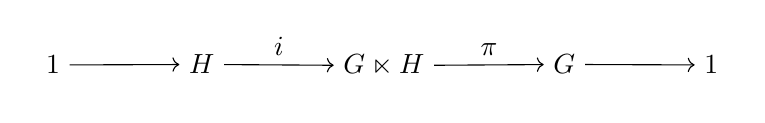
\begin{tikzpicture}
%\matrix(m)[matrix of math nodes, row sep=3em, column sep=3em, text height=1.5ex, text depth=0.25ex]
\matrix(m)[matrix of math nodes, row sep=4em, column sep=4em]
{
	1   &  H &  G \ltimes H & G & 1 \\
};
%\path[->,font=\scriptsize]
\path[->]
(m-1-1) edge node[auto]{$$} (m-1-2)
(m-1-2) edge node[auto]{$i$} (m-1-3)
(m-1-3) edge node[auto]{$\pi$} (m-1-4)
(m-1-4) edge node[auto]{$$} (m-1-5)	
;
\end{tikzpicture} 
\end{equation}
with 
\begin{equation}
	\begin{aligned}
	& i : H\to G \ltimes H \\ 
	& i(x) = (x,1)
\end{aligned}
\end{equation}
$i$ group homomorphism, since 
\[
i(x_1x_2) = (x_1x_2 ,1) = (x_1 \tau(1)x_2 , 1) = (x_1,1)\cdot (x_2,1) = i(x_1)i(x_2)
\]
\begin{equation}
	\begin{aligned}
	& \pi : G \ltimes H \to G\\ 
	& \pi(x,g) = g 
\end{aligned}
\end{equation}
cf. \url{http://sierra.nmsu.edu/morandi/oldwebpages/math683fall2002/GroupExtensions.pdf}

Observe that 
\[
\pi i(x) = \pi(x,1)=1 \text{ so } \text{ker}\pi = \text{im}i
\]

\begin{definition}[Semi-direct product (2); with direct product]\label{Def:Semidirectprod2}
	\textbf{direct product} $G=HK$ if \\
$H,K$ subgroups of group $G$, s.t. \\
\begin{itemize}
\item $H$ and $K$ are normal in $G$ ($gkg^{-1} \in K$ \, $\forall \, g\in G$, $\forall \, k \in K$)  
\item $H\cap K = \lbrace 1 \rbrace$  
\item $HK=G$.  
\end{itemize} 

\textbf{semi-direct product}.  Relax the 1st condition (of direct products) so $H$ still normal in $G$, but $K$ need not be.  \\
\begin{itemize}
\item $H$ normal in $G$ ($ghg^{-1} \in H, \, \forall \, g , \, \forall \, h \in H$)  
\item $H\cap K = \lbrace 1 \rbrace$ 
\item $HK = G$
\end{itemize}
\end{definition}

\emph{Connection between} Def. \ref{Def:Semidirectprod} and Def. \ref{Def:Semidirectprod2} for the \emph{semidirect product}:  Consider $\tau : G \to \text{Aut}(H)$.  

Consider $G \ltimes H$ - what is the identity $1_{G\ltimes H} \equiv (1_H,1_G)$ of this group?  
\[
(x,g)\cdot (1_H,1_G) = (x\tau(g) 1_H, g1_G) = (x\tau(g)1_H, g) \Longrightarrow 1_H = \tau(g^{-1})1, \, 1_G=1
\]
and so the inverse, $\forall (x,g) \in G\ltimes H$, $(x,g)^{-1} \equiv ((x^{-1}), (g^{-1}))$, 
\[
\begin{gathered}
	(x,g) (x,g)^{-1} = (x\tau(g) (x^{-1}),g(g^{-1}) ) = (x\tau(g)(x^{-1}), 1) \text{ (if $(g^{-1}) = g^{-1}$) }
\end{gathered}
\]
Moving along, 
\[
\begin{gathered}
	x\tau(g) (x^{-1}) = \tau(g^{-1})1 \\
\Longrightarrow (x^{-1}) = \tau(g^{-1}) x^{-1}\tau(g^{-1})1
\end{gathered}
\]

Checking out the $H$ being a normal subgroup of $G\ltimes H$ condition, i.e. $H \lhd G$, 
\[
\begin{gathered}
	(x,g)(h,1)(\tau(g^{-1})x^{-1} \tau(g^{-1}) , g^{-1}) = (x\tau(g)h, g)(\tau(g^{-1})x^{-1}\tau(g^{-1}) , g^{-1}) = \\
= (x\tau(g)h \tau(g)\tau(g^{-1}) x^{-1}\tau(g^{-1}), 1) = (x\tau(g) hx^{-1}\tau(g^{-1}), 1) 
\end{gathered}
\]
$\Longrightarrow$ $H$ normal subgroup of $G\ltimes H \equiv H \lhd (G\ltimes H)$.  

\href{http://www.math.columbia.edu/~bayer/S09/ModernAlgebra/semidirect.pdf}{Notes on Semidirect products}
\item extension 
\begin{equation}
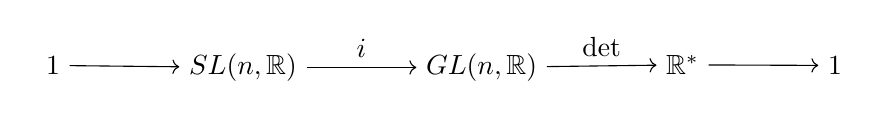
\begin{tikzpicture}
%\matrix(m)[matrix of math nodes, row sep=3em, column sep=3em, text height=1.5ex, text depth=0.25ex]
\matrix(m)[matrix of math nodes, row sep=4em, column sep=4em]
{
	1   &  SL(n,\mathbb{R}) &  GL(n,\mathbb{R}) & \mathbb{R}^* & 1 \\
};
%\path[->,font=\scriptsize]
\path[->]
(m-1-1) edge node[auto]{$$} (m-1-2)
(m-1-2) edge node[auto]{$i$} (m-1-3)
(m-1-3) edge node[auto]{$\text{det}$} (m-1-4)
(m-1-4) edge node[auto]{$$} (m-1-5)	
;
\end{tikzpicture} 
\end{equation}

with \\
$GL(n,\mathbb{R}) \equiv Gl_n(\mathbb{R}) = \lbrace A | A \in \text{Mat}_{\mathbb{R}}(n,n); \text{det}A \neq 0\rbrace$ \\
$\text{det}:GL(n,\mathbb{R}) \to \mathbb{R}^* \equiv \mathbb{R} \backslash \lbrace 0 \rbrace $, $\text{det}$ surjective homomorphism \\
$SL(n,\mathbb{R}) \equiv Sl_n(\mathbb{R}) = \lbrace A | A \in \text{Mat}_{\mathbb{R}}(n,n); \, \text{det}A=1\rbrace$ \\

Note that $\text{ker}(\text{det}) = SL(n,\mathbb{R})$.  

Now 
\[
\mathbb{R}^* \simeq \lbrace a 1_n | a \in \mathbb{R}^* \rbrace
\]
and $\text{det}(a1_n) = a^n$.  

If $n$ odd, and $\text{det}(a1_n)=a^n =1$, then $a=1$.  If $n$ even, $a=\lbrace -1, 1 \rbrace$.  

By the second definition of a semi-direct product, Def. \ref{Def:Semidirectprod2}, it's required that $SL(n,\mathbb{R}) \cap \mathbb{R}^* = 1$ (i.e. the intersection is only the identity).  This will only be the case if $n$ odd.  

cf. \url{http://sierra.nmsu.edu/morandi/oldwebpages/math683fall2002/GroupExtensions.pdf}

\end{itemize}

\part{Quantum Mechanics}

\section{The Wave function and the Schr\"{o}dinger Equation, its probability interpretation, some postulates}

cf. Ch. 2 "The Wave Function and the Schr\"{o}dinger Equation" in \textbf{Quantum Mechanics} by Franz Schwabl (2007) \cite{FrSc2007}.

From experimental considerations (Sec. 1.2.2, Schwabl (2007) \cite{FrSc2007}), with electron diffraction, electrons, $e^-$, have wavelike properties; let this wave be $\psi(\mathbf{x}, t)$. 

For free $e^-$ of momentum $\mathbf{p}$, energy $E = \frac{ \mathbf{p}^2}{2m}$, in accordance with diffraction experiments, consider as free plane waves 
\[
\psi(\mathbf{x}, t) = C \exp{ \left( i ( \mathbf{k} \cdot \mathbf{x} - \omega t)\right)}, \qquad \, \omega = E / \hbar = E, \, \mathbf{k} = \mathbf{p}/ hbar = \mathbf{p}
\]
with $\hbar = 1$

Hypothesis: wave function $\psi(\mathbf{x},t)$ gives probability distribution 
\[
\rho(\mathbf{x}, t) = | \psi(\mathbf{x}, t)|^2
\]
$\rho(\mathbf{x}, t) d^3 x = $ probability of finding $e^-$ at location $\mathbf{x}$ in volume element $d^3x$.

e.g. $e^-$ waves $\psi_1(\mathbf{x}, t)$ , $\psi_2(\mathbf{x},t)$

If both slits open, superposition of wave functions $\psi_1(\mathbf{x}, t) + \psi_2(\mathbf{x},t)$

Note $| \psi_1(\mathbf{x},t) + \psi_2(\mathbf{x},t) |^2 \neq | \psi_1(\mathbf{x},t) |^2 + |\psi_2(\mathbf{x},t) |^2$ if there are no interference terms.

Important remarks: 

\begin{enumerate}
	\item[(i)] Single $e^-$ not smeared out. $\rho(\mathbf{x},t)$ is \textbf{not} the charge distribution of $e^-$, but is the probability density for measuring particle at position $\mathbf{x}$ at time $t$.
	\item[(ii)] Prob. distribution doesn't occur by interference of many simultaneously incoming $e^-$, but one obtains same interference pattern if each $e^-$ enters separately, i.e. even for very low intensity source. Thus, wave function applies to every electron and describes state of single $e^-$.
\end{enumerate}

cf. 2.2 "The Schr\"{o}dinger Equation for Free Particles" in \textbf{Quantum Mechanics} by Franz Schwabl (2007) \cite{FrSc2007}.

(i) 1st. order DE (differential equation); (ii) linear in $\psi$ for linear superposition (iii) "homogeneous" $\int d^3x | \psi(\mathbf{x}, t) |^2 = 1$, (iv) plane waves
\[
\psi(\mathbf{x},t) = C \exp{ \left[ i (\mathbf{p} \cdot \mathbf{x} - \frac{p^2}{2m} t)/ \hbar\right]} \qquad \, \text{ plane waves }
\]
Should be solutions of the equations.

From postulates (i-iv),
\[
i \hbar \frac{\partial}{ \partial t} \psi(\mathbf{x}, t) = \frac{ -\hbar^2}{2m } \nabla^2 \psi(\mathbf{x},t)
\]
Time-dependent Schr\"{o}dinger equation for free particles.

\[
\int_{-\infty}^{\infty} d^3k e^{i\mathbf{k} \cdot \mathbf{x}} e^{-k^2 \alpha^2} = \prod_{j=x}^z \int_{-\infty}^{\infty} dk_j e^{ik_j x_j} e^{-k_j^2 \alpha^2}  = \prod_{j=x}^z \left( \sqrt{ \frac{\pi}{\alpha^2} } \exp{ \left( \frac{-x_j^2}{4\alpha^2} \right)} \right) = \left( \frac{\sqrt{\pi}}{\alpha} \right)^3 \exp{ \left( \frac{-x^2}{4\alpha^2} \right)}
\]


\part{Algebraic Topology}  

cf. Bredon (1997) \cite{Bred1997}


\section{Simplicial Complexes}  

cf. pp. 245, from Sec. 21 Simplicial Complexes of Ch. 4 Homology Theory in Bredon (1997) \cite{Bred1997}

$\mathbf{v}_0, \dots \mathbf{v}_n \in \mathbb{R}^{\infty}$, "affinely independent" if they span an affine $n$-plane, i.e. 
\[
\text{ if } \left( \sum_{i=0}^n \lambda_i \mathbf{v}_i =0 , \, \sum_{i=0}^n \lambda_i = 0 \right), \text{ then } \Longrightarrow \forall \, \lambda_i = 0
\]
If not, then, e.g. $\lambda_0 \neq 0$, assume $\lambda_0 =-1$, and solve the equations to get 

\[
\begin{gathered}
\mathbf{v}_0 = \sum_{i=1}^n \lambda_i \mathbf{v}_i \\
\sum_{i=1}^n \lambda_i = 1
\end{gathered}
\]
i.e. $\mathbf{v}_0$ is in affine space spanned by $\mathbf{v}_1\dots \mathbf{v}_n$.  

If $\mathbf{v}_0, \dots \mathbf{v}_n$ affinely independent, then 
\begin{equation}
\sigma = ( \mathbf{v}_0, \dots \mathbf{v}_n) = \lbrace \sum_{i=0}^n \lambda_i \mathbf{v}_i | \sum_{i=0}^n \lambda_i = 1, \, \lambda_i \geq 0 \rbrace
\end{equation}
is "affine simplex" spanned by $\mathbf{v}_i$; also convex hull of $\mathbf{v}_i$.  

$\forall \, k \leq n$, $k$-face of $\sigma$ is any affine simplex of form $(\mathbf{v}_{i_1}, \dots \mathbf{v}_{i_k})$, where vertices all distinct, so are affinely independent.  

\begin{definition}
	(geometric) simplicial complex $K:= $ collection of affine simplices s.t. \begin{enumerate}
		\item $\sigma \in K \Longrightarrow $ any face of $\sigma \in K$; and 
		\item $\sigma, \tau \in K \Longrightarrow \sigma \bigcap \tau $ is a face of both $\sigma$ and $\tau$, or $\sigma \bigcap \tau =\emptyset$
	\end{enumerate}

If $K$ simplicial complex, $|K| = \bigcup \lbrace \sigma | \sigma \in K \rbrace \equiv $ "polyhedron" of $K$
\end{definition}

\begin{definition}[Def. 21.2 of Bredon (1997) \cite{Bred1997}]
	polyhedron $:= $ space $X$ if $\exists \, $ homeomorphism $h: |K| \xrightarrow{ \approx } X$ for some simplicial complex $K$.  
	$h,K$ is triangulation of $X$; (map $h$, complex $K$)
\end{definition}

Let $K$ finite simplicial complex.  \\
Choose ordering of vertices $\mathbf{v}_0,\mathbf{v}_1\dots $ of $K$.  \\
If $\sigma = (\mathbf{v}_{\sigma_0}, \dots \mathbf{v}_{\sigma_n})$ is simplex of $K$, where $\sigma_0 < \dots < \sigma_n$, then  \\
\phantom{If } let $f_{\sigma} : \Delta_n \to |K|$ be 
\[
f_{\sigma} = [\mathbf{v}_{\sigma_b}, \dots \mathbf{v}_{\sigma_n}]
\]
in notation of Def. 1.2.  Bredon (1997) \cite{Bred1997}.  

Then this gives CW-complex structure on $|K|$ with $f_{\sigma}$ as characteristic maps.  




\part{Graphs, Finite Graphs}

\section{Graphs, Finite Graphs, Trees }

Serre (1980) \cite{Serr1980}  

cf. Chapter I. Trees and Amalgams, Section 1 Amalgams, Subsection 1.1 Direct limits of Serre (1980) \cite{Serr1980}  


Let $(G_i)_{i\in I}$, family of groups.    

$\forall \, $ pair $(i,j)$, let $F_{ij} = $ set of homomorphisms of $G_i$ into $G_j$

Want: group $G= \varinjlim G_i$ and 
\[
\lbrace f_i | f_i : G_i \to G \rbrace \text{s.t. } f_j \circ f = f_i \quad \, \forall \, f \in F_{ij}
\]
group $G$ and family $\lbrace f_i\rbrace$ universal in that  

(*) if $H$ group, if $\lbrace h_i | h_i :G_i \to H ; h_j \circ f = h_i \qquad \, \forall \, f \in F_{ij} \rbrace$, \\
then $\exists \, ! h: G\to H$ s.t. $h_i = h\circ f_i$  \\
i.e. $\text{Hom}(G,H) \simeq \varprojlim \text{Hom}(G_i,H)$, the inverse limit being taken relative to $F_{ij}$.  \\
i.e. $G$ direct limit of $G_i$ relative to the $F_{ij}$.  

EY : 20170918 this is my rewrite/reinterpretation:

Let $(G_i)_{i\in I}$, $\forall \, (i,j) \in I^2$, let $F_{ij} = \lbrace f \equiv f_{ij} | f:G_i \to G_j , f \text{ homomorphism of $G_i$ into $G_j$ } \rbrace$.  

Given group $G = \varinjlim G_i$ (for fixed $i$), $\lbrace f_i | f_i : G_i \to G  |  f_j \circ f = f_i \quad \, \forall \, f \in F_{ij} \rbrace$, i.e.  

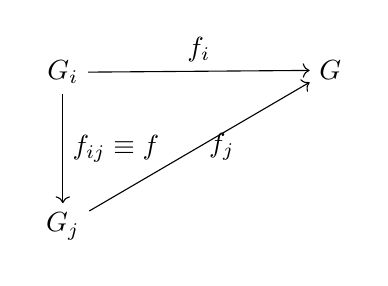
\begin{tikzpicture}
\matrix(m)[matrix of math nodes, row sep=4em, column sep=8em]
{
G_i    &  G   \\
G_j   &  \\};
\path[->]
(m-1-1) edge node[auto]{$f_i$} (m-1-2)
edge node[auto]{$f_{ij} \equiv f$} (m-2-1) 
(m-2-1) edge node[right]{$ f_j$ } (m-1-2);
\end{tikzpicture} 

Then $G$,  $\lbrace f_i | f_i : G_i \to G  |  f_j \circ f = f_i \quad \, \forall \, f \in F_{ij} \rbrace$ \textbf{universal} \\
\phantom{Then } if $\forall \, $ group $H$, $\forall \, \lbrace h_i |  h_i : G_i \to H  | h_j \circ f = h_i \quad \, \forall \, f \in F_{ij} \rbrace$, \\
\phantom{Then if } then $\exists \, ! \  h : G\to H$, s.t. $h_i = h \circ f_i$ i.e. 
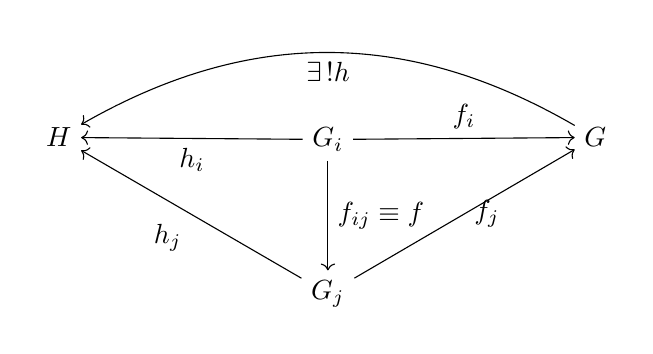
\begin{tikzpicture}
\matrix(m)[matrix of math nodes, row sep=4em, column sep=8em]
{
H & G_i    &  G   \\
& G_j   &  \\};
\path[->]
(m-1-2) edge node[auto]{$f_i$} (m-1-3)
edge node[auto]{$f_{ij} \equiv f$} (m-2-2) 
edge node [auto]{$h_i$} (m-1-1)
(m-2-2) edge node[right]{$ f_j$ } (m-1-3)
edge node [auto]{$h_j$} (m-1-1) 
(m-1-3) edge[bend right = 30] node [auto]{ $\exists \, ! h$ } (m-1-1)  
;
\end{tikzpicture} 






\begin{proposition}
	$\exists \, !$ pair $G$, family $(f_i)_{i\in I}$, i.e. (pair consisting of $G, (f_i)_{i\in I}$, unique up to unique isomorphism.  
\end{proposition}
\begin{proof}
Define $G$ by generators and relations.  \\
Take generating family to be disjoint union of those for $G_i$.  \\
relations - $xyz^{-1}$ where $x,y,z \in G_i$, $z=xy \in G_i$ \\
\phantom{relations - } $xy^{-1}$ where $x\in G_i$, $y \in G_j$, $y=f(x)$ for at least $f\in F_{ij}$.  

Thus, existence of $G,\lbrace f_i\rbrace$.  

$G$ represents functor $H\mapsto \varprojlim \text{Hom}{(G_i,H)}$.  

Thus, uniqueness (also from universal property).  
\end{proof}

e.g. groups $A,G_1,G_2$, homomorphisms $\begin{aligned} & \quad \\ 
& f_1 : A \to G_1 \\
& f_2 : A \to G_2 
\end{aligned}$.  

$G$ obtained by amalgamating $A$ in $G_1,G_2$ by $f_1,f_2 \equiv G_1 *_A G_2$.  \\
1 can have $G=\lbrace 1 \rbrace$, even though $f_1,f_2$ non-trivial.  

\emph{Application}: (Van Kampen Thm.)

Let topological space $X$ be covered by open $U_1,U_2$.   \\
Suppose $U_1,U_2, U_{12}=U_1\bigcap U_2$ arcwise connected.  

Let basept. $x\in U_{12}$.  

Then $\pi_1(X;x)$ obtained by taking 3 groups 
\[
\pi_1(U_1;x), \pi_1(U_2;x), \pi_1(U_{12};x)
\]
and amalagamating them according to homomorphism
\[
\begin{aligned}
& \pi_1(U_{12};x) \to \pi_1(U_1;x)  \\
& \pi_1(U_{12};x) \to \pi_1(U_2;x)
\end{aligned}
\]

\exercisehead{1}  
Let homomorphisms $\begin{aligned} & \quad \\
	& f_1 : A \to G_1 \\ 
	& f_2: A \to G_2 \end{aligned}
$
amalgam $G=G_1 *_A G_2$.  

Define subgroups $A^n,G_1^n, G_2^n$, of $A,G_1,G_2$ recursively by 
\[
\begin{aligned}
& A^1 = \lbrace 1 \rbrace \\
& G_1^1 = \lbrace 1 \rbrace \\ 
& G_2^1 = \lbrace 1 \rbrace \\ 
\end{aligned}
\]

$A^n = $ subgroup of $A$ generated by $f_1^{-1}(G_1^{n-1})$ and $f_2^{-1}(G_2^{n-1})$  
\[
G_1^n = \text{subgroup of $G_i$ generated by $f_i(A^n)$ }
\]

Let $A^{\infty}, G_i^{\infty}$ be unions of $A^n, G_i^n$ resp.  

Show that $f_i$ defines injection $A/A^{\infty} \to G_i/G_i^{\infty}$.  

So the amalgamation is $G \simeq G_1/G_1^{\infty} *_{A/A^{\infty}} G_2/G_2^{\infty}$.  

Take the first induction case (for intuition about the solution).  

\[
\begin{aligned}
	& A^2 = \langle f_1^{-1}( G_1^1), f_2^{-1}(G_2^1) \rangle = \langle f_1^{-1}(\lbrace 1 \rbrace), f_2^{-1}(\lbrace 1 \rbrace ) \rangle \\
	& G_i^2 = f_i(A^2)
\end{aligned}
\]
Let $f_i(a) = f_i(b) \in G_i/G_i^{\infty}$; $a,b\in A/A^{\infty}$.  

Then since $f_i(a),f_i(b) \in G_i/G_i^{\infty}$, $f_i(a),f_i(b) \in \lbrace gG_i^{\infty} | g\in G_i \rbrace$ (quotient is defined to be the set of all left cosets of $G_i^{\infty}$, which has to be a normal subgroup for $G_i/G_i^{\infty}$ to be a quotient group).  

Since $a,b \in A/A^{\infty}$, suppose we take $a,b\in A$.  

And suppose we take 
\[
\begin{aligned}
& 	f_i(a) = f_i(a)G_i^{\infty} = f_i(a) f_i(A^{n_a} ) = f_i(aA^{n_a}) \\ 
& 	f_i(b) = f_i(b)G_i^{\infty} = f_i(b) f_i(A^{n_b} ) = f_i(bA^{n_b})  
\end{aligned}
\]
Taking $f_i^{-1}$ (recall for group homomorphisms, they map inverse of element of 1st. group to inverse of image of this element).  

$aA^{n_a}=bA^{n_b}\in A/A^{\infty}$ (This is okay as we've "quotiented out $A^{\infty}$; so indeed, they're equal)


cf. Subsection 1.2 Structure of amalgams of Serre (1980) \cite{Serr1980} 

Suppose given group $A$, family of groups $(G_i)_{i\in I}$, and, $\forall \, i\in I$, injective homomorphism $A\to G_i$.  

$*_A G_i \equiv $ direct limit (cf. no. 1.1) of family $(A,G_i)$ with respect to these homomorphisms, call it \emph{sum} (in category theory sense, i.e. product) of $G_i$ with $A$ amalgamated.  

e.g. $A=\lbrace 1 \rbrace$, \\
$*G_i \equiv $ free product of $G_i$.  

\subsubsection{reduced word}  

$\forall \, i \in I$, choose set $S_i$ of right coset representations of $G_i$ modulo $A$, 

assume $1 \in S_i$, 

$(a,s)\mapsto as$ is bijection of $A\times S_i$ onto $G_i$,  \\
$A\times (S_i-\lbrace 1 \rbrace) \to G_i-A$ (onto)

Let $\mathbf{i} = (i_1\dots i_n)$, $n\geq 0$, $i_j \in I$, s.t. 
\begin{equation}
i_m \neq i_{m+1} \text{ for } 1 \leq m \leq n-1
\end{equation}
cf. (T) of Serre (1980) \cite{Serr1980}.  

So \emph{reduced word} $m$ is defined as 
\[
m = (a;s_1\dots s_n)
\]
where $a\in A, s_1\in S_{i_1} \dots s_n \in S_{i_n}$, and $s-j \neq 1\, \forall \, j$.  

$f\equiv $ canonical homomorphism of $A$ into group $G= *_A G_i$ \\ 
$f_i \equiv $ canonical homomorphism of $G_i$ into group $G= *_A G_i$

EY : 20170611 (Further explanations, basic examples, from me):  

Given $A, \lbrace G_i\rbrace_{i\in I}$, injective (group) homomorphisms $\lbrace f_i: A \to G_i\rbrace_i$.  

$G_i \backslash f_i(A) = \lbrace f_i(A)g | g\in G_i\rbrace$.  

Right coset representation of $f_i(A)g\mapsto g$.  

e.g. $A,G_1,G_2$, $\begin{aligned} & \quad \\
	& f_1:A \to G_1 \\
		& f_2 : A\to G_2 \end{aligned}$.  
		
	\[
	\begin{aligned}
	& G_1\backslash f_1(A) = \lbrace f_1(A)g| g\in G_1\rbrace \\
	& G_2\backslash f_2(A) = \lbrace f_2(A)g | g\in G_2 \rbrace
	\end{aligned}
	\]

$\mathbf{i} = (i_1\dots i_n)$, $i_j\in I$, $i_m\neq i_{m+1}$ for $1\leq m \leq n-1$.  

Consider $(1212\dots 12)$  

$m=(a;f_1 g_2 f_3 g_4 \dots f_{2n-1}, g_{2n})$ where $f$'s $\in S_1 \subset G_1$, $g$'s $\in S_2 \subset G_2$.  

and so 
\begin{definition}[reduced word]
	\textbf{reduced word} of type $\mathbf{i}$, $m$, \begin{equation}
	m=(a;s_1\dots s_n)
	\end{equation}
	where $a\in A, s_1 \in S_{i_1}, \dots s_n \in S_{i_n}$, $s_j\neq 1$ \, $\forall \, j$, \\
	\phantom{where } $\mathbf{i} = (i_1\dots i_n)$, $i_j \in I$, s.t. $i_m \neq i_{m+1}$ for $1\leq m \leq n-1$, \\
	with $S_i = \lbrace g | g\in f_i(A)g \in f_i(A) G_i\rbrace$  
\end{definition}




\begin{theorem}[1 of Serre (1980) \cite{Serr1980} ]
	$\forall \, g \in G$, $\exists \, $ sequence $\mathbf{i}$ s.t. $i_m \neq i_{m+1}$ for $1\leq m \leq n-1$ and 
	
	reduced word 
	\[
	m = (a;s_1\dots s_n) 
	\]
	of type $\mathbf{i}$ s.t. 
	\[
	g = f(a)f_{i_1}(s_1) \dots f_{i_n}(s_n)
	\]
\end{theorem}

Furthermore, $\mathbf{i}$ and $m$ unique.  

\emph{Remark}.  Thm. 1 implies $f;f_i$ injective.  

Then identify $A$ and $G_i$ with images $f(A), f_i(G_i)$ in $G$, and reduced decomposition (*) of $g\in G$ 
\[
g = as_1\dots s_n, \quad \, a\in A, \, s_1 \in S_{i_1} - \lbrace 1 \rbrace \dots s_n \in S_{i_n} - \lbrace 1 \rbrace
\]
Likewise, $G_i \bigcap G_j = A$ if $i\neq j$.  

In particular, $S_i - \lbrace 1 \rbrace$ pairwise disjoint in $G$.  

\begin{proof}
Let $X_i \equiv $set of reduced words of type $\mathbf{i}$, $X = \coprod X_i$.  

Make $G$ act on $X$.  

In view of universal property of $G$, sufficient to make $\forall \, i, G_i$ act, 

check action induced on $A$ doesn't depend on $i$  

Suppose then that $i\in I$, and let $Y_i = $ set of reduced words of form $(1;s_1 \dots s_n)$, with $i_1\neq i$.  

EY : 20170611

Recall that 
\[
S_i = \lbrace g| g\in f_i(A) g \in f_i(A) G_i \rbrace
\]
\[
\begin{aligned}
	& A \times S_i \to G_i \text{ onto } \\ 
	& A\times (S_i - \lbrace 1 \rbrace) \to G_i - A \text{ onto } \\ 
	& (a,s) \mapsto as \text{ bijection }
\end{aligned}
\]

Let $Y_i = $ set of reduced words of form $(1; s_1 \dots s_n) = \lbrace (1;s_1 \dots s_n) | 1\in A; s_1 \in S_{i_1}\dots s_n \in S_{i_n} ; \mathbf{i} = (i_1\dots i_n), \, i_j \in I \text{ s.t. } i_m \neq i_{m+1} \text{ for } 1\leq m \leq n -1 \rbrace$.  

\[
\begin{gathered}
\begin{gathered}
A \times Y_i \to X = \coprod_i X_i \\
(a,(1; s_1 \dots s_n)) \mapsto (a; s_1 \dots s_n)
\end{gathered} \\
\begin{gathered}
A\times \lbrace S_i - \lbrace 1 \rbrace ) \times Y_i \to X \\
((a,s), (1;s_1 \dots s_n)) \mapsto (a;s,s_1\dots s_n)
\end{gathered}
\end{gathered}
\]
and remember that $X_i = $ set of reduced words of type $\mathbf{i}$.  

It's clear that this yields a bijection $A\times Y_i \bigcup A\times (S_i - \lbrace 1 \rbrace) \times Y_i \to X$.  

Let $x\in X$.  Then $x\in X_{\mathbf{i}}$ for some $\mathbf{i}$.  So $x$ is a reduced word of type $\mathbf{i}$: $x = (a;s_1\dots s_n)$.  Then clearly $x = (a;s_1\dots s_n) \mapsto (a,(1;s_1\dots s_n)) \in A\times Y_i$.  







\end{proof}


cf. pp. 13, Sec. 2. Trees, 2.1 Graphs of Serre (1980) \cite{Serr1980}

\begin{definition}[1. of Serre (1980) \cite{Serr1980}]
	\textbf{graph} $\Gamma = (X,Y, Y\to X\times X, Y\to Y)$, where $\begin{aligned} & \quad \\
		& \text{ set } X = \text{ vert } \Gamma \\ 
		& \text{ set } Y = \text{ edge } \Gamma \end{aligned}$  

\[
\begin{aligned}
& Y \to X\times X \\ 
& y\mapsto (o(y), t(y)) \\
& Y\to Y \\
& y\mapsto \overline{y}
\end{aligned}
\]
s.t. $\forall \, y \in Y$, $\overline{ \overline{y}} = y$, $\overline{y} \neq y$, $o(y) = t(\overline{y})$.  

vertex $P \in X$ of $\Gamma$. 

(oriented) edge $y\in Y$, $\overline{y} \equiv $ inverse edge.  

origin of $y := $ vertex $o(y) = t(\overline{y})$.  

terminus of $y:= $ vertex $t(y) = o(\overline{y})$   

extremities of $y:= \lbrace o(y),t(y)\rbrace$  

If 2 vertices \textbf{adjacent}, they're extremities of some edge.  

orientation of graph $\Gamma = Y_+ \subset Y = \text{ edge } \Gamma$ s.t. $Y = Y_+ \coprod \overline{Y}_+$.  It always exists.  

oriented graph defined, up to isomorphism, by giving 2 sets $X,Y_+$ and $Y+ \to X\times X$.  
	
	corresponding set of edges is $Y = Y_+\coprod \overline{Y}_+$ where $\overline{Y}_+ \equiv $ copy of $Y_+$  
\end{definition}

\subsubsection{Realization of a Graph}

cf. Realization of a Graph in Serre (1980) \cite{Serr1980}.  

Let graph $\Gamma$, $X = \text{vert}\Gamma$, $Y = \text{edge}\Gamma$.

topological space $T = X \coprod Y \times [0,1]$, where $X,Y$ provided with discrete topology.  

Let $R$ be finest equivalence relation on $T$ for which 
\begin{equation}
\begin{gathered} \begin{aligned}
	& (y,t) \equiv (\overline{y}, 1-t) \\ 
	& (y,0) \equiv o(y) \\
	& (y,1) \equiv t(y)
\end{aligned} \qquad \, \forall \, y \in Y, \, \forall \, t \in [0,1]
\end{gathered}
\end{equation}

quotient space $\text{real}(\Gamma) = T/R $ is \emph{realization} of graph $\Gamma$.  (realization is a functor which commutes with direct limits).  

Let $n\in \mathbb{Z}^+$.  Consider oriented graph of $n+1$ vertices $0,1,\dots n$,  \\

\begin{definition}
	path (of length $n$) in graph $\Gamma$ is morphism $c$ of $\mathbf{\text{Path}}_n$ into $\Gamma$  
\end{definition}

orientation given by $n$ edges $[i,i+1]$, $0\leq i <n$, $\begin{aligned} & \quad \\
& o([i,i+1]) = i \\
& t([i,i+1]) = i+1 \end{aligned}$  

For $n\geq 1$, \\
$(y_1\dots y_n)$ sequence of edges $y_i = c([i-1,i])$ s.t. 
\[
t(y_i) = o(y_{i+1}), \qquad \, 1 \leq i < n \text{ determine } c
\]
If $P_i = c(i)$,  \\
$c$ is a path from $P_0$ to $P_n$, and $P_0$ and $P_n$ are \emph{extremities of the path $c$}.  

pair of form $(y_i,y_{i+1})=(y_i, \overline{y}_i)$ in path is \textbf{backtracking}.  

path (of length $n-2$), from $P_0$ to $P_n$ given (for $n>2$) by $(y_1\dots y_{i-1}, y_{i+2}\dots y_n)$  

If $\exists \, $ path from $P$ to $Q$ in $\Gamma$, $\exists \, $ one without backtracking (by induction)  

direct limit $\mathbf{\text{Path}}_{\infty} = \varinjlim \mathbf{\text{Path}}_n$ provides notion of infinite path.  \\
$\mathbf{\text{Path}}_{\infty} \ni $ infinite sequence $(y_1,y_2 , \dots)$ of edges s.t. $t(y_i) = o(y_{i+1})$ \, $\forall \, i \geq 1$.  


\begin{definition}[connected graph; Def. 3 of Serre (1980) \cite{Serr1980}]
	graph connected if $\forall \, $ 2 vertices, 2 vertices are extremities of at least 1 path.  
	
	maximal connected subgraphs (under relation of inclusion) are \emph{connected components} of graph.  
\end{definition}

\subsubsection{Circuits}  

Let $n\in \mathbb{Z}^+$, $n\geq 1$.  

Consider \\
set of vertices $\mathbb{Z}/n\mathbb{Z}$, orientation given by $n$ edges $[i,i+1]$, $(i\in \mathbb{Z}/n\mathbb{Z})$ with $\begin{aligned} & \quad \\
 & o([i,i+1]) = i \\
 & t([i,i+1]) = i+1 \end{aligned}$

\begin{definition}[circuit; Def. 4 of Serre (1980) \cite{Serr1980}]
	circuit (length $n$) in graph is subgraph isormorphic to $\mathbf{\text{Circ}}_n$.  
\end{definition}
i.e. subgraph = path $(y_1\dots y_n)$, without backtracking, s.t. $P_i = t(y_i)$, \, $(1\leq i \leq n)$ distinct, s.t. $P_n = o(y_1)$

$n=1$ case: $\mathbf{\text{Circ}}_1$, $\mathbb{Z}/\mathbb{Z} = \lbrace 0 \rbrace$, $1$ edge, $[0,1]$, $0 \in \mathbb{Z}/1\mathbb{Z}$, $\begin{aligned} & \quad \\
	& o([0,1]) = 0 \\
	& t([0,1]) = 1 \end{aligned}$  
	
	Note $\mathbf{\text{Circ}}_1$ has automorphism of order 2, which changes its orientation, i.e. \\
	$\exists \, $ automorphism $\sigma \in \text{Aut}( \mathbf{\text{Circ}}_1) $ s.t. $|\sigma | = 2$, i.e. $\sigma^2=1$.  \\
	loop $:= $ circuit of length $1$; so loop $\in \overline{ \mathbf{\text{Circ}} }_1$.  
	
	path $(y_1)$, $P_1 = t(y_1) = o(y_1)$.  
	
	$n=2$ case: $\mathbf{\text{Circ}}_2$, $\mathbb{Z}/2\mathbb{Z} = \lbrace 0 ,1\rbrace$, 2 edges $[0,1], [1,2]$,  \\
	path $(y_1,y_2)$, $(1\leq i \leq 2)$, $\begin{aligned} & \quad \\
		& P_1 = t(y_1) \\
		& P_2 = t(y_2) = o(y_1) \end{aligned}$  
		
		
	

\subsection{Combinatorial graphs}

Let $(X,S)\equiv $ simplicial complex of dim. $\leq 1$, with \\
$X \equiv $ set \\
$S \equiv $ set of subsets of $X$ with $1$ or $2$ elements, containing all the 1-element subsets.  

associates with it a graph $\Gamma = (X, \lbrace (P,Q) \rbrace)$.  

$X$ is its set of vertices.  

edges $=\lbrace (P,Q)\in X\times X\rbrace$ s.t. $P\neq Q$, $\lbrace P ,Q \rbrace \in S$, with $\overline{(P,Q)} = (Q,P)$
\[
\begin{aligned}
& o(P,Q) = P \\
& t(P,Q) = Q
\end{aligned}
\]

In this graph, 2 edges with same origin and same terminus are equal.  This is equivalent to (see following Def.)

\begin{definition}[combinatorial; Def. 5 of Serre (1980) \cite{Serr1980}]
	graph is combinatorial if it has no circuit of length $\leq 2$
\end{definition}
Conversely, it's easy to see that 

every combinatorial graph $\Gamma$ derived (up to isomorphism) by construction above from simplicial complex $(X,S)$, where \\
$X = \text{vert} \Gamma$ \\
$S=$ set of subset $\lbrace P,Q \rbrace$ of $X$ s.t. $P$ and $Q$ either adjacent or equal. 

\part{Tensors, Tensor networks; Singular Value Decomposition, QR decomposition, Density Matrix Renormalization Group (DMRG), Matrix Product states (MPS)}

\section{Introductions to Tensor Networks}

Jos\'{e} Barbon (IFT-CSIC, Univ. Autonoma de Madrid) gave the \href{Workshop introductory overview}{https://youtu.be/nsxgAOAEgbg} for the workshop "Black Holes, Quantum Information, Entanglement, and all that," (29 May-1 June, 2017, with the organizing committee of Thibault Damour (IHES), Vasily Pestun (IHES), Eliezer Rabinovici (IHES \& Hebrew Univ. of Jerusalem).  

In the talk, 


cf. \href{https://youtu.be/nsxgAOAEgbg?t=43m13s}{43:13}  

\subsection*{The church of the doubled Hilbert space}
 
Any thermal box can be obtained by tracing over a second identical copy, if appropriately entangled into a global pure state.  

\[
\rho_R = \text{Tr}_L \sum_n C_n \Psi_n^L \otimes \Psi_n^R
\]
\[
(C_n)_{\text{thermal}} = \left[ \frac{ e^{-\beta E_n} }{ \sum_m e^{-\beta E_M} } \right]^{1/2}
\]

But!!

If the entanglement basis is taken to be the high-energy band of two "entangled" CFTs ... 
\[
|TFD \rangle \sim \sum_{E_n} e^{-\beta E_n/2} | E_n \rangle_L \otimes | E_n \rangle_R
\]
neglecting the tiny $e^{-S}$ spacings. we can approximate by continuous spectrum of fields in the background of an AdS black hole, to get ... 
 
\[
\int_E e^{-\beta E/2} |E\rangle_L \otimes | E\rangle_R 
\]
The HH state of the bulk fields!  

cf. \href{https://youtu.be/nsxgAOAEgbg?t=46m16s}{46:16}

SLOGAN: EPR $=$ ER
Maldacena-Susskind  

Accumulating a density of entanglement of $S \gg 1$ well-separated Bell pairs within a transversal size of order $(GS)^{1/2}$  seems to generate a geometrical bridge of area $GS$.  



cf. \href{https://youtu.be/nsxgAOAEgbg?t=49m26s}{49:26}  

\subsection*{Parametrizing complexity of entanglement}

Pick a tensor decomposition of Hilbert space of dimension $\exp{(S)}$ into $S$ factors of $O(1)$ dimension.  
\[
\mathcal{H} = \mathcal{H}_1 \otimes \mathcal{H}_2 \otimes \dots \otimes \mathcal{H}_S
\]
A tensor of S indices gives a generic state.  

cf. \href{https://youtu.be/nsxgAOAEgbg?t=50m27s}{50:27}  

The decomposition of the big tensor in small building blocks gives a notion of "complexity of entanglement"  

rather simple entanglement pattern  

somewhat more complex entanglement pattern

picture from M von Raamsdonk  

cf. \href{https://youtu.be/nsxgAOAEgbg?t=55m10s}{55:10}

\subsection*{A list of open questions \& problems}

\begin{itemize}
\item Need exactly calculable toy models of AdS/CFT along the lines of SYK model  
\item Give a "renormalized" definition of quantum complexity for continuum CFTs 
\item Can tensor networks describe bulk gravitons?  
\item What is the space-time meaning of quantum complexity saturation?  
\item Can we define approximate local observables for black hole inferiors?  
\item Are there obstructions related to firewalls and/or fuzzballs?   
\end{itemize}

\href{https://youtu.be/nsxgAOAEgbg}{Workshop introductory overview } by Jos\'{e} Barbon for the \href{https://www.youtube.com/channel/UC4R1IsRVKs_qlWKTm9pT82Q}{Institut des Hautes Études Scientifiques (IHÉS)} gave me the first impetus to understand tensor networks as I sought to also understand the condensates of entanglement pairs within the black hole.  

A Google search for introductions to tensor networks that are on arxiv ("Introduction Tensor Network arxiv") yielded Bridgeman and Chubb's course notes (bf. Bridgeman and Chubb (2017) \cite{BrCh2017}).    

\subsection{List of stuff I want to look at/do/study}  
I would like to compare/contrast the following:  
\begin{itemize}
\item Rotman (2010) \cite{JRotman2010}, Ch. 8, but starting from 8.4 Tensor Products, pp. 574  
\item Jeffrey Lee (2009) \cite{JLee2009}, Ch. 7 Tensors 
\item \url{http://www.irisa.fr/sage/bernard/publis/SVD-Chapter06.pdf}, \url{https://math.stackexchange.com/questions/694339/parallel-algorithms-for-svd}
\end{itemize}



Maldacena and Susskind (2013) \cite{MaSu2013}  

Lectures on Gravity and Entanglement.  Mark Van Raamsdonk  \cite{Raam2016}

\begin{itemize}
\item Consider as physical system AdS-Schwarzchild black hole   
\item CFT 
\begin{itemize}
\item \href{https://arxiv.org/pdf/1601.05000.pdf}{PFL Lectures on Conformal Field Theory in $D\geq 3$ Dimensions}, Rychkov (2016) \cite{Rych2016}.  
\end{itemize}
\end{itemize}

Evenbly and Vidal (2011) \cite{EvVi2011}, Tensor network states and geometry

Loose ends (might not be useful links)
\begin{itemize}
\item \url{https://arxiv.org/pdf/1506.06958.pdf}
\item \url{https://arxiv.org/pdf/1512.02532.pdf} One-point Functions in AdS/dCFT from Matrix Product States
\end{itemize}

Numerical implementation strategy: 1st, CUDA cuSolver, 2nd, Numerical Recepes version, 3rd, parallel algorithm review.


\subsection{Tensor operations; Tensor properties}

\subsubsection{rank}

$r=$ rank tensor of dim. $d_1\times \dots \times d_r$ is element of $\mathbb{C}^{d_1\times \dots \times d_r}$  

Tensor product
\begin{equation}
	[A \otimes B]_{i_1 \dots i_r, j_1 \dots j_s } := A_{i_1 \dots i_r} \cdot B_{j_1 \dots j_s }
\end{equation}

\subsubsection{Trace}
Given tensor $A$, $x$th, $y$th indices have identical dims. ($d_x = d_y$), \\
partial trace over these 2 dims. is simply joint summation over that index
\begin{equation}
	[\text{Tr}_{x,y} A]_{i_1\dots i_{x-1}i_{x+1} \dots i_{y-1}i_{y+1} \dots i_r} = \sum_{\alpha=1}^{d_x} A_{i_1 \dots i_{x-1} \alpha i_{x+1} \dots i_{y-1} \alpha i_{y+1} \dots i_r}
\end{equation}

\subsubsection{Contraction}

\subsubsection{Group and splitting, Bridgeman and Chubb (2017) \cite{BrCh2017} }

"Rank is a rather fluid concept in the study of tensor networks."  Bridgeman and Chubb (2017) \cite{BrCh2017}.  

$\mathbb{C}^{a_1 \times \dots \times a_n} \simeq \mathbb{C}^{b_1 \times \dots \times b_m}$ isomorphic as vector spaces if $\prod_i a_i = \prod_i b_i$.  

We can "group" or "split" indices to lower or raise rank of given tensor, resp.  

Consider contracting 2 arbitrary tensors.  

If we group together indices which are and are not involved in contraction, \\
"It should be noted that not only is this reduction to matrix multiplication pedagogically handy, but this is precisely the manner in which numerical tensor packages perform contraction, allowing them to leverage highly optimised matrix multiplication code." (cf. Bridgeman and Chubb (2017) \cite{BrCh2017}; check this)

"Owing to freedom in choice of basis, precise details of grouping and splitting aren't unique." (cf. Bridgeman and Chubb (2017) \cite{BrCh2017}).  

1 specific choice of convention:  \\
tensor product basis, defining basis on product space by product of respective bases.  

"The canonical use of tensor product bases in quantum information allows for grouping and splitting described above to be - dealt with implicitly."  


\begin{equation}
 | 0 \rangle \otimes | 1 \rangle \equiv | 0 \rangle 
\end{equation} and precisely this grouping, 
\begin{equation}
\begin{gathered}
	| 0 \rangle \otimes | 1 \rangle \in \text{Mat}_{\mathbb{C}}(2,2), \text{ whilst } \\ 
 | 0 1 \rangle \in \mathbb{C}^4  
\end{gathered}
\end{equation}

Suppose rank $n+m$ tensor $T$, group its first $n$ indices, last $m$ indices together.
\[
T_{I,J} := T_{i_1\dots i_n,j_1\dots j_m}
\]
where 
\[
\begin{aligned}
	& I := i_1 + d_1^{(i)} i_2 + d_1^{(i)}  d_2^{(i)} i_3 + \dots + d_1^{(i)} \dots d_{n-1}^{(i)} i_n \\ 
	& J := j_1 + d_1^{(j)} j_2 + d_1^{(j)}  d_2^{(j)} j_3 + \dots + d_1^{(j)} \dots d_{m-1}^{j)} j_m 
\end{aligned}
\]

EY : 20170627 to elaborate, consider a functor \verb|flatten| that does what's described above, in the context of category theory (and so this is the generalization):

\begin{equation}
\begin{gathered}
	\mathbb{K}^{d_1^{(i)} } \times \mathbb{K}^{d_2^{(i)} } \times \dots \times \mathbb{K}^{d_n^{(i)} } \times \mathbb{K}^{d_1^{(j)} } \times \mathbb{K}^{d_2^{(j)} } \times \dots \times \mathbb{K}^{d_m^{(j)} } \xrightarrow{ \text{ flatten } } \mathbb{K}^{ \prod_{p=1}^n d_p^{(i)} } \times \mathbb{K}^{ \prod_{q=1}^m d_q^{(j)} }   \\
T_{i_1 \dots i_n, j_1 \dots j_m } \xmapsto{ \text{ flatten } } T_{I,J}   \\
\lbrace 0 ,1, \dots d_1^{(i)} \rbrace \times \lbrace 0 ,1, \dots d_2^{(i)} \rbrace \times \dots \times \lbrace 0 ,1, \dots d_n^{(i)} \rbrace \times \lbrace 0 ,1, \dots d_1^{(j)} \rbrace \times \lbrace 0 ,1, \dots d_2^{(j)} \rbrace \times \dots \times \lbrace 0 ,1, \dots d_m^{(j)} \rbrace \xrightarrow{ \text{ flatten } } \\
\xrightarrow{ \text{ flatten } }  \lbrace 0 ,1, \dots  \prod_{p=1}^n d_p^{(i)} -1 \rbrace \times \lbrace 0 ,1, \dots \prod_{q=1}^m d_q^{(j)} - 1 \rbrace  \\
(i_1,i_2, \dots i_n, j_1,j_2 \dots j_m ) \xmapsto{ \text{ flatten } } (I,J) := (i_1 + d_1^{(i)} i_2 + \dots + d_1^{(i)} \dots d_{n-1}^{(i)} i_n ,j_1 + d_1^{(j)} j_2 + \dots + d_1^{(j)} \dots d_{m-1}^{(j)} j_m ) \\ 
\end{gathered}
\end{equation}
It doesn't make sense to call this "row-major" or "column-major" ordering generalization, because we are not dealing with only 2 indices where we can definitely say the first index indexes the "row" and the second index indexes the "column."  At most, possibly, you can alternatively have this:
\[
(i_1 \dots i_n,j_1\dots j_m) \xmapsto{ \text{ flatten } } (I,J) := (d_2^{(i)} \dots d_n^{(i)}i_1 + d_3^{(i)} \dots d_n^{(i)} i_2 + \dots + i_n , d_2^{(j)} \dots d_m^{(j)} j_1 + \dots + j_m )
\]
Note that this is all \emph{$0$-based counting} (i.e. we start counting from $0$ just like in C,C++,Python, etc.).  If you really wanted $1$-based counting, you'd have to complicate the above formulas as such:
\[
\begin{gathered}
(I,J) := (i_1 + d_1^{(i)} (i_2-1) + \dots + d_1^{(i)} \dots d_{n-1}^{(i)} (i_n-1) ,j_1 + d_1^{(j)} (j_2-1) + \dots + d_1^{(j)} \dots d_{m-1}^{(j)} (j_m-1) ) \\ 
\end{gathered}
\]
Note that formulas are easily checked by pluggin in the minimum and maximum values for the indices and seeing if they make sense (e.g. plug in $(0,0,\dots ,0)$ for all indices for $0$-based counting and make sure you get back $I=0$ or $J=0$).  

\subsection{Singular Value Decomposition}  

\begin{equation}
\begin{gathered}
	T_{I,J} = \sum_{\alpha} U_{I,\alpha} S_{\alpha,\alpha} \overline{V}_{J,\alpha} \\ 
 \text{Mat}_{\mathbb{K}}(N,M) \xrightarrow{ \text{ SVD } } \text{Mat}_{\mathbb{K}}(N,P) \times \text{Mat}_{\mathbb{K}}(P,P) \times \text{Mat}_{\mathbb{K}}(M,P)    \\
	T_{I,J} \xmapsto{ \text{ SVD } } U_{I,\alpha}, S_{\alpha,\alpha} , \overline{V}_{I,\alpha} \text{ s.t. } \\
T_{I,J} = \sum_{\alpha} U_{I,\alpha} S_{\alpha, \alpha} \overline{V}_{J,\alpha}    \\
T=USV^{\dag}
\end{gathered}
\end{equation}
For the higher-dimensional version of SVD, 
\begin{equation}
\begin{gathered}
	\mathbb{K}^{d_1^{(i)} } \otimes \dots \otimes \mathbb{K}^{d^{(i)}_N} \otimes \mathbb{K}^{d_1^{(j)} }\otimes \dots \otimes \mathbb{K}^{d_M^{(j)} }  \xrightarrow{ \text{ flatten } } \text{Mat}_{\mathbb{K}}(N,M) \xrightarrow{ \text{ SVD } }     \text{Mat}_{\mathbb{K}}(N,P) \times \text{Mat}_{\mathbb{K}}(P,P) \times \text{Mat}_{\mathbb{K}}(M,P) \xrightarrow{ \text{ splitting } } \\ 
\xrightarrow{ \text{ splitting } } \mathbb{K}^{d_1^{(i)} } \otimes \dots \otimes \mathbb{K}^{d^{(i)}_N} \otimes \mathbb{K}^P \times \text{Mat}_{\mathbb{K}}(P,P) \times  \mathbb{K}^{d_1^{(j)} }\otimes \dots \otimes \mathbb{K}^{d_M^{(j)} } \otimes \mathbb{K}^P  \\
T_{i_1\dots i_N,j_1 \dots j_M} = \sum_{\alpha} U_{i_1\dots i_N,\alpha} S_{\alpha,\alpha} \overline{V}_{j_1 \dots j_M, \alpha}
\end{gathered}
\end{equation}

\section{Density Matrix Renormalization Group; Matrix Product States (MPS)}

\subsection{Introduction; physical system (physical setup)}

cf. "Density Matrix Renormalization Group/Matrix Product States" lectures by Schollw\"{o}ck (2017) \cite{ArSo2017}.

Recall the fundamental Hamiltonian (frequently in solid state physics), for \emph{electrons moving in a Hamiltonian potential}. 
\begin{equation}
H = \sum_{j=1}^{ e^-} \frac{\mathbf{p}_j^2}{ 2m_e} + \frac{1}{2} \frac{1}{ 4\pi \epsilon_0} \frac{q_e^2}{ |\mathbf{r}_i - \mathbf{r}_j|^2 } + \sum_{j=1}^{e^-} V_{\text{eff}}(\mathbf{r}_j)
\end{equation}
where $\frac{\mathbf{p}_j^2}{ 2m_e}$ is the kinetic energy term, $\sum_{j=1}^{e^-} V_{\text{eff}}(\mathbf{r}_j)$ is the lattice potential.
The problem is in the 2nd. term, electron-electron interaction, $\frac{1}{2} \frac{1}{ 4\pi \epsilon_0} \frac{q_e^2}{ |\mathbf{r}_i - \mathbf{r}_j|^2 }$

Typical models include the following:

\begin{itemize}
	\item Hubbard model (tight, binding-like model; basis states are not energy states but \emph{Wannier basis} states):
	\begin{equation}
	H = -t \sum_{ \langle i, j \rangle, \sigma } c^{\dag}_{i \sigma} c_{j \sigma} + h.c. + U \sum_i n_{i \uparrow} n_{i \downarrow }
	\end{equation}
	where $\langle i, j \rangle$ denotes nearest neighbors, $\sigma$ index is for all possible states, $h.c.$ stands for hermitian conjugate, and \\
	$d \equiv$ number of states of single spin site. \\
	$-t \sum_{ \langle i, j \rangle, \sigma } c^{\dag}_{i \sigma} c_{j \sigma} + h.c.$ is the kinetic energy term, \\
	$U \sum_i n_{i \uparrow} n_{i \downarrow }$ is the Coulomb energy.
	
	Hilbert space for the Hubbard model is 
	\begin{equation}
	\lbrace | \emptyset \rangle , | \uparrow \rangle , | \downarrow \rangle , | \uparrow \downarrow \rangle \rbrace^{ \otimes L}, \qquad \, d = 4
	\end{equation}
	\item Heisenberg model (large -$U$ Hubbard at half-filling)
	\begin{equation}
	H = J \sum_{ \langle i , j \rangle } \mathbf{S}_i \cdot \mathbf{S}_j = J \sum_{ \langle i, j \rangle } \frac{1}{2} (S_i^{+} S_j^- + S_j^{+} S_i^-) + S_i^z S_j^z  )
	\end{equation}
	Hilbert space $\lbrace | \uparrow \rangle, | \downarrow \rangle \rbrace^{\otimes L}$, $d=2$ 
\end{itemize}

\subsubsection{Compression of information viewpoint for solid-state Hamiltonians, quantum many-body systems}.

"emergent" macroscopic quantities, $\tau, p$ (temperature, pressure). For 
\[
	H = J \sum_{ \langle i , j \rangle } \mathbf{S}_i \cdot \mathbf{S}_j = J \sum_{ \langle i, j \rangle } \frac{1}{2} (S_i^{+} S_j^- + S_j^{+} S_i^-) + S_i^z S_j^z  )
\]

$H$ as classical spins: thermodynamic limit $N \to \infty$. 2 angles required to describe unit vector on unit sphere ($S^3$) $\Longrightarrow 2N $ degrees of freedom (linear)

quantum spins: superposition of states, thermodynamic limit: $N \to \infty$, $2^N$ degrees of freedom (exponential).

\subsubsection{Definitions; notation and conventions}

Quantum system living on $L$ lattice sites; cf. Schollw\"{o}ck (2017) \cite{ArSo2017}, lattice can be in any dim., effectively most useful in 1-dim., think of the example of a 1-dim. chain of $L$ sites. \\

$d$ local states per site $\lbrace \sigma_i \rangle$, $i \in \lbrace 1,2, \dots L\rbrace$

e.g. spin $\frac{1}{2}$, $d=2$, $| \uparrow \rangle, | \downarrow \rangle$.

Hilbert space: $\mathcal{H} = \otimes_{i=1}^L \mathcal{H}_i$, $\mathcal{H}_i = \lbrace | 1_i \rangle , \dots | d_i \rangle \rbrace$. 

Notice, there are \emph{exponentially many coefficients}, $c$'s. Most general state (not necessarily 1-dim.) is 
\begin{equation}
|\psi \rangle = \sum_{\sigma_1 \dots \sigma_L} c^{\sigma_1 \dots \sigma_L} | \sigma_1 \dots \sigma_L \rangle
\end{equation}

abbreviations: $\lbrace \sigma \rbrace = \sigma_1 \dots \sigma_L$. And so we can write $c^{\lbrace \sigma \rbrace}$. 

\subsection{MPS, matrix product states}

\begin{equation}
| \psi \rangle = \sum_{\sigma_1 \dots \sigma_L} M^{\sigma_1} M^{\sigma_2} \dots M^{\sigma_L} | \sigma_1 \sigma_2 \dots \sigma_L \rangle
\end{equation}

The $\sum_{\sigma_1 \dots \sigma_L}$ means that all basis states participate; Schollw\"{o}ck is not kicking out any states arbitrarily. 
\[
c^{\lbrace \sigma \rbrace} = M^{\sigma_1} M^{\sigma_2} \dots M^{\sigma_L} \in \mathbb{C}
\] so

$M^{\sigma_1} \in \text{Mat}_{\mathbb{C}}(1, n_1)$ so to get a scalar in the product of matrices. Likewise, $M^{\sigma_L} \in \text{Mat}_{\mathbb{C}}(m_L, 1)$

(variational) constraint is in expansion coefficients. 

$\forall \, $ $d$ local basis states, $|\sigma_i \rangle \in V_i \equiv V$,$\text{dim}V = d$, let there be 1 matrix $M$, i.e. $M^{\sigma_i}$.  \\
Thus, $dL$ matrices altogether (in total).

Assume matrix size has upper limit $D$ (a computer limitation).

Up to $dLD^2$ coefficients, instead of exponentially many ($c^{\lbrace \sigma \rbrace}$, and sum over $\lbrace \sigma \rbrace$). 

\subsubsection{Product States and MPS}

Mean-filed approximation/product state misses essential quantum feature: \textbf{entanglement}. 

Consider 2 spin $\frac{1}{2}$ systems: $\mathcal{H} = \mathcal{H}_1 \otimes \mathcal{H}_2$, $\mathcal{H}_i = \lbrace | \uparrow \rangle, | \downarrow \rangle \rbrace$

General state is 
\[
| \psi \rangle = c^{ \uparrow \uparrow} | \uparrow \uparrow \rangle + c^{ \uparrow \downarrow} | \uparrow \downarrow \rangle + c^{ \downarrow \uparrow} | \downarrow \uparrow \rangle + c^{ \downarrow \downarrow} | \downarrow \downarrow \rangle 
\]

e.g. singlet state: $|\psi \rangle = \frac{1}{ \sqrt{2} } | \uparrow \downarrow \rangle - \frac{1}{ \sqrt{2} } | \downarrow \uparrow \rangle $. 

As an exercise, show that the singlet state cannot be written as product of local coefficients, i.e. 
\[
c_{\uparrow \downarrow } \neq c^{\uparrow} c^{ \downarrow }
\]

Instead of writing products of scalars, write product of matrices, i.e. $e^{\sigma_1} \cdot e^{\sigma_2} \to M^{\sigma_1} M^{\sigma_2}$

\[
\begin{gathered}
\begin{aligned}
	& M^{\uparrow 1} = \left[ \begin{matrix} 1 & 0 \end{matrix} \right]
	& M^{\downarrow 1} = \left[ \begin{matrix} 0 & 1 \end{matrix} \right] 
	\end{aligned} \quad \quad \, \begin{aligned}
	& M^{\uparrow 2 } = \left[ \begin{matrix} 0 \\ \frac{-1}{\sqrt{2}} \end{matrix} \right] \\
	& M^{\downarrow 2} = \left[ \begin{matrix} \frac{1}{\sqrt{2}} \\ 0 \end{matrix} \right] 
	\end{aligned}
\end{gathered}
\]

\[
\begin{gathered}
M^{\uparrow 1} M^{\downarrow 2} = \frac{1}{\sqrt{2}} \\ 
M^{\downarrow 1} M^{\uparrow 2} = \frac{-1}{\sqrt{2}} 
\end{gathered}
\]

\subsubsection{AKLT model (Affleck-Kennedy-Lieb-Tasaki)}

MPS is useful even for matrices of dim. 2.


\subsection{General matrix product state (MPS) and SVD (Singular Value Decomposition)}

cf. Schollw\"{o}ck (2017) \cite{ArSo2017}

The general matrix product state (MPS) is the following:
\begin{equation}
|\psi \rangle = \sum_{ \sigma_1 \dots \sigma_L } M^{\sigma_1} M^{\sigma_2} \dots M^{\sigma_L} | \sigma_1 \sigma_2 \dots \sigma_L \rangle
\end{equation}
where $\sigma_i \in V_i$, $\text{dim}V_i = d_i$ and \\
$M^{\sigma_1} \in \text{Mat}_{\mathbb{C}}(1, D_1)$ \\ 
$M^{\sigma_2} \in \text{Mat}_{\mathbb{C}}(D_1, D_2)$ \\ 
$\vdots$ \\ 
$M^{\sigma_{L-1}} \in \text{Mat}_{\mathbb{C}}(D_{L-2}, D_{L-1})$ \\ 
$M^{\sigma_L} \in \text{Mat}_{\mathbb{C}}(D_{L-1}, 1)$ \\ 

Notice the non-unique \textbf{gauge degree of freedom}:

$\forall \, A \in \text{Mat}_{\mathbb{C}}(m,n)$, then for $k = \min{(m,n)}$, 
\begin{equation}
\begin{gathered}
A = U SV^{\dagger} \equiv U \Sigma V^{\dagger} \text{ where }
\end{gathered}
\end{equation}

$U \in \text{Mat}_{\mathbb{C}}(m,k)$, $U^{\dagger} U =1$ (i.e. $U$ consists of orthonormal columns, or $k$ number of $u$'s $\in \mathbb{C}^m$); if $m=k$, $UU^{\dagger} = 1$, \\
$S \in \text{Mat}_{\mathbb{C}}(k,k)$ s.t. $S \in \text{diag}_{\mathbb{C}}(k)$, $s_1 \geq s_2 \geq s_3 \geq \dots s_i \geq 0$, $s_j$'s non-negative "singular values" (adjacent "singular" in name doesn't imply anything), non-vanishing = $\text{rank} r \leq k$. \\
$V^{\dagger} \in \text{Mat}_{\mathbb{C}}(k,n)$, $V^{\dagger} V = 1$, (orthonormal rows, or $k$ number of $v\in \mathbb{C}^n$); if $k=n $, $VV^{\dagger} = 1$

Recall eigenvalue equation and thus so-called eigenvalue decomposition.

For $A \in \text{Mat}_{\mathbb{C}}(m,m)$, 
\[
\begin{gathered}
	Au_j = \lambda_j u_j ; \qquad \, j =1 \dots r ; \, r \equiv \text{ rank }, \quad \, u_j \in \text{Mat}_{\mathbb{C}}(m, 1) \\
	A_{ik} u_{kj} = \lambda_j u_{ij} = u_{ik} \delta_{kj} \lambda_j \Longrightarrow AU = U \Lambda
\end{gathered}
\]
with $U \in \text{Mat}_{\mathbb{C}}(m, r)$, $\Lambda \in \text{Mat}_{\mathbb{C}}(r, r)$.

And so
\[
\begin{gathered}
\begin{aligned}
& AA^{\dagger} = USV^{\dagger} VSU^{\dagger} = US^2 U^{\dagger} \Longrightarrow (AA^{\dagger})U = US^2 \\ 
& A^{\dagger} A = VSU^{\dagger} U SV^{\dagger} = VS^2 V^{\dagger} \Longrightarrow (A^{\dagger}A)V = VS^2
\end{aligned}
\end{gathered}
\]
so if we treat $U$ and $V$, matrices of left, right singular vectors, then $S^2$ singular value squared are eigenvalues.

Start with 

\begin{equation}
| \psi \rangle = \sum_{\sigma_1 \dots \sigma_L} c^{\sigma_1 \dots \sigma_L} | \sigma_1 \dots \sigma_L \rangle \in V \text{ s.t. } \text{dim} V = d^L
\end{equation}

Note the \emph{abuse of notation}: while $c^{\sigma_1 \dots \sigma_L} \in \mathbb{C}$ itself, also denote $c^{\sigma_1 \dots \sigma_L} \in \mathbb{C}^{d^L}$ as a shorthand for $\sum_{\sigma_1 \dots \sigma_L} c^{\sigma_1 \dots \sigma_L} | \sigma_1 \dots \sigma_L \rangle$

Reshape coefficient vector into matrix of (size) dimension ($d\times d^{L-1}$). 
\[
\begin{gathered}
\mathbb{C}^{d^L} \xrightarrow{\text{reshape}} \text{Mat}_{\mathbb{C}}(d, d^{L-1}) \\
c^{\sigma_1 \dots \sigma_L} \xmapsto{\text{reshape}} \Psi_{\sigma_1, (\sigma_2 \dots \sigma_L)} 
\end{gathered}
\]

Then do SVD:
\[
\Psi_{\sigma_1, (\sigma_2 \dots \sigma_L)}  \stackrel{ \text{SVD} }{=} \sum_{a_1} U_{\sigma_1 a_1} S_{a_1 a_1} V^{\dagger}_{a_1, \sigma_2 \dots L} = U_{\sigma_1 a_1} S_{a_1 a_1 } V^{\dagger}_{a_1, \sigma_2 \dots \sigma_L}
\]


Let's utilize commutative diagrams to summarize the reshaping and SVD operations that we've done.

\[
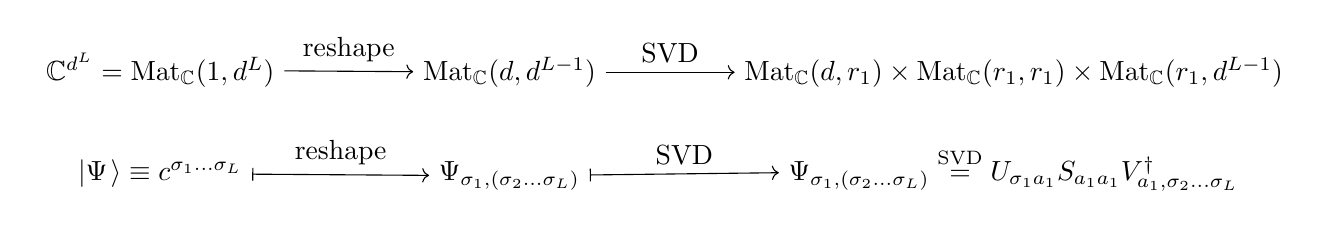
\begin{tikzpicture}
\matrix (m) [matrix of math nodes, row sep=1.55em, column sep=4.7em, minimum width=3.2em]
{
	\mathbb{C}^{d^L} = \text{Mat}_{\mathbb{C}}(1, d^L) & \text{Mat}_{\mathbb{C}}(d, d^{L-1}) & \text{Mat}_{\mathbb{C}}(d, r_1) \times \text{Mat}_{\mathbb{C}}(r_1, r_1) \times \text{Mat}_{\mathbb{C}}(r_1 , d^{L-1}) \\
	\left| \Psi \right. \rangle \equiv c^{\sigma_1 \dots \sigma_L} & \Psi_{\sigma_1, (\sigma_2 \dots \sigma_L) } & \Psi_{\sigma_1, (\sigma_2 \dots \sigma_L) } \stackrel{\text{SVD}}{=} U_{\sigma_1 a_1 } S_{a_1 a_1} V^{\dagger}_{a_1, \sigma_2 \dots \sigma_L} \\
};
\path[->]
(m-1-1) edge node [above] { \text{reshape} } (m-1-2)
(m-1-2) edge node [above] { \text{SVD} } (m-1-3)
;
\path[|->]
(m-2-1) edge node [above] { \text{reshape} } (m-2-2)
(m-2-2) edge node [above] { \text{SVD} } (m-2-3)
;
\end{tikzpicture}  
\]
where I abuse notation for the SVD operation in that, SVD maps a matrix (in this case, $\Psi$) into 3 matrices, that obey the equality relationship when they're multiplied together (i.e. $\Psi = USV^{\dagger}$). 


Slice $U$ into $d$ row vectors, i.e. for $U \in \text{Mat}_{\mathbb{C}}(d,r_1)$.
\[
\begin{gathered}
\begin{aligned}
\text{Mat}_{\mathbb{C}}(d, r_1) & \xrightarrow{\text{slice}} \text{Mat}_{\mathbb{C}}(1, r_1)^d \\
U_{\sigma_1 a_1} & \mapsto \lbrace A^{\sigma_1} \rbrace \equiv \lbrace A^{\sigma_1}_{1, a_1} \rbrace_{\sigma_1} \text{ s.t. } A^{\sigma_1}_{1,a_1} = U_{\sigma_1 a_1} \text{ and } | \lbrace A^{\sigma_1}_{1, a_1} \rbrace | = d
\end{aligned}
\end{gathered}
\]

Collecting all the operations, and doing the following notation rewrite,
\[
\begin{gathered}
c^{\sigma_1 \sigma_2 \dots \sigma_L} \mapsto \Psi_{\sigma_1 \sigma_2 \dots \sigma_L} = \sum_{a_1} A^{\sigma_1}_{1 a_1} S_{a_1 a_1} V^{\dagger}_{a_1, \sigma_2 \dots \sigma_L} = \sum_{a_1} A^{\sigma_1}_{1a_1} c^{a_1 \sigma_2 \sigma_3 \dots \sigma_L}
\end{gathered}
\]
where
\[
c^{a_1 \sigma_2 \sigma_3 \dots \sigma_L} = S_{a_1 a_1} V^{\dagger}_{a_1 \sigma_2 \dots \sigma_L}
\]

Do the same procedure again. 

\[
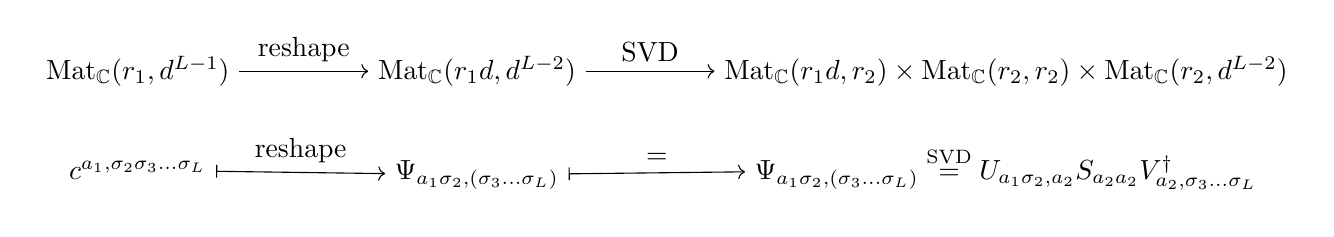
\begin{tikzpicture}
\matrix (m) [matrix of math nodes, row sep=1.55em, column sep=4.7em, minimum width=3.2em]
{
	\text{Mat}_{\mathbb{C}}(r_1, d^{L-1}) & \text{Mat}_{\mathbb{C}}(r_1d, d^{L-2}) & \text{Mat}_{\mathbb{C}}(r_1d, r_2) \times \text{Mat}_{\mathbb{C}}(r_2, r_2) \times \text{Mat}_{\mathbb{C}}(r_2 , d^{L-2}) \\
	c^{a_1, \sigma_2 \sigma_3 \dots \sigma_L} & \Psi_{a_1\sigma_2, (\sigma_3 \dots \sigma_L) } & \Psi_{a_1 \sigma_2, (\sigma_3 \dots \sigma_L) } \stackrel{\text{SVD}}{=} U_{a_1 \sigma_2, a_2 } S_{a_2 a_2} V^{\dagger}_{a_2, \sigma_3 \dots \sigma_L} \\
};
\path[->]
(m-1-1) edge node [above] { \text{reshape} } (m-1-2)
(m-1-2) edge node [above] { \text{SVD} } (m-1-3)
;
\path[|->]
(m-2-1) edge node [above] { \text{reshape} } (m-2-2)
(m-2-2) edge node [above] { = } (m-2-3)
;
\end{tikzpicture}  
\]

Then slice $U$ into $d$ matrices, and then matrix multiply the $S$ and $V^{\dagger}$ matrices together:
\[
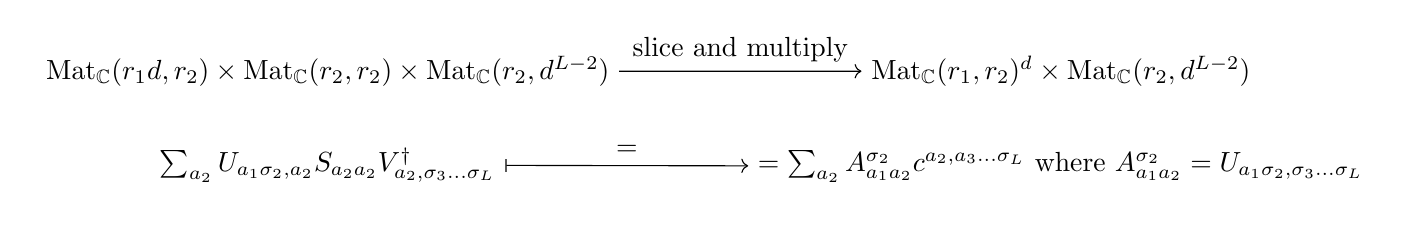
\begin{tikzpicture}
\matrix (m) [matrix of math nodes, row sep=1.55em, column sep=4.7em, minimum width=3.2em]
{
	\text{Mat}_{\mathbb{C}}(r_1d, r_2) \times \text{Mat}_{\mathbb{C}}(r_2, r_2) \times \text{Mat}_{\mathbb{C}}(r_2 , d^{L-2}) & \text{Mat}_{\mathbb{C}}(r_1, r_2)^d \times \text{Mat}_{\mathbb{C}}(r_2, d^{L-2}) \\
	\sum_{a_2} U_{a_1 \sigma_2, a_2 } S_{a_2 a_2} V^{\dagger}_{a_2, \sigma_3 \dots \sigma_L} & = \sum_{a_2} A^{\sigma_2}_{a_1 a_2} c^{a_2, a_3 \dots \sigma_L} \text{ where } A^{\sigma_2}_{a_1 a_2} = U_{a_1\sigma_2, \sigma_3 \dots \sigma_L } \\
};
\path[->]
(m-1-1) edge node [above] { \text{slice and multiply} } (m-1-2)
;
\path[|->]
(m-2-1) edge node [above] { = } (m-2-2)
;
\end{tikzpicture}  
\]

\end{multicols*}
%\begin{multicols*}{1}


Thus, generalize the \emph{$i$th procedure}: for $i = 1 \dots L$, 

Let $r_0 = 1$.

\begin{equation}\label{Eq:LeftMPSoperation}
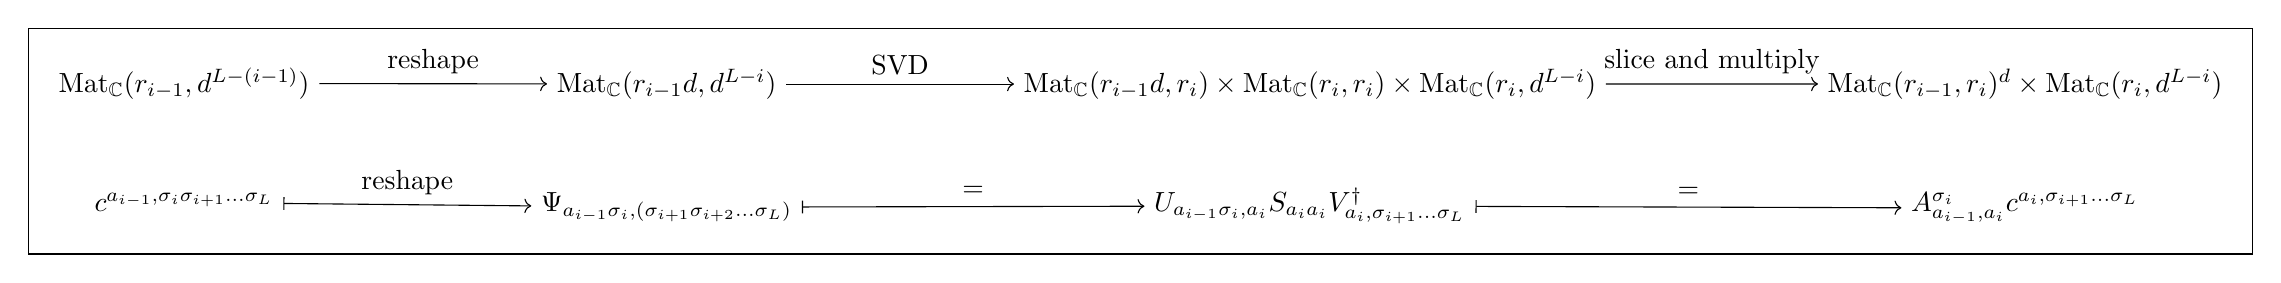
\begin{tikzpicture}[framed]
\matrix (m) [matrix of math nodes, row sep=2.55em, column sep=7.7em, minimum width=6.2em]
{
	\text{Mat}_{\mathbb{C}}(r_{i-1}, d^{L-(i-1)}) & \text{Mat}_{\mathbb{C}}(r_{i-1}d, d^{L-i}) & \text{Mat}_{\mathbb{C}}(r_{i-1}d, r_i) \times \text{Mat}_{\mathbb{C}}(r_i, r_i) \times \text{Mat}_{\mathbb{C}}(r_i , d^{L-i}) & \text{Mat}_{\mathbb{C}}(r_{i-1}, r_i)^d \times \text{Mat}_{\mathbb{C}}(r_i, d^{L-i}) \\
	c^{a_{i-1}, \sigma_i \sigma_{i+1} \dots \sigma_L} & \Psi_{a_{i-1}\sigma_i, (\sigma_{i+1} \sigma_{i+2} \dots \sigma_L) } &  U_{a_{i-1} \sigma_i, a_i } S_{a_i a_i} V^{\dagger}_{a_i, \sigma_{i+1} \dots \sigma_L} & A^{\sigma_i}_{a_{i-1}, a_i} c^{a_i, \sigma_{i+1} \dots \sigma_L} \\
};
\path[->]
(m-1-1) edge node [above] { \text{reshape} } (m-1-2)
(m-1-2) edge node [above] { \text{SVD} } (m-1-3)
(m-1-3) edge node [above] { \text{slice and multiply} } (m-1-4)
;
\path[|->]
(m-2-1) edge node [above] { \text{reshape} } (m-2-2)
(m-2-2) edge node [above] { = } (m-2-3)
(m-2-3) edge node [above] { = } (m-2-4)
;
\end{tikzpicture}  
\end{equation}

Remember that $r_i \leq \min{(r_{i-1} d, d^{L-i})} $ and for $i=L$, there is no need to do a SVD, but only a reshape, and slice and multiply.

Collecting all the $A$ matrices:

\begin{equation}
\boxed{
	\begin{gathered}
\begin{aligned}
& A^{\sigma_1}_{1, a_1} \in \text{Mat}_{\mathbb{C}}(1,r_1); \qquad \, r_1 \leq d \\
& A^{\sigma_2}_{a_1, a_2} \in \text{Mat}_{\mathbb{C}}(r_1,r_2); \qquad \, r_2 \leq r_1 d \\
& \vdots \\
& A^{\sigma_i}_{a_{i-1}, a_i} \in \text{Mat}_{\mathbb{C}}(r_{i-1},r_i); \qquad \, r_i \leq \min{(r_{i-1}d, d^{L-i})} \\
& \vdots \\
& A^{\sigma_L}_{a_{L-1}, a_L} \in \text{Mat}_{\mathbb{C}}(r_{L-1}, 1); \qquad \, r_{L-1} \leq d
\end{aligned}
	\end{gathered}}
\end{equation}

\begin{multicols*}{2}

\subsubsection{Left and Right Normalization, $A$ and $B$ matrices, "special gauge" from normalization}

Choose orthonormal basis states $\forall \, a_l, \, \forall \, l = 1, 2, \dots L$
For
\[
\begin{aligned}
& | a_l \rangle = \sum_{ a_{l-1} \sigma_l } M^{\sigma_l}_{a_{l-1}a_l } | a_{l-1} \sigma_l \rangle \\
& \langle a_l' | = \sum_{a'_{l-1} \sigma_l'} \langle a'_{l-1} \sigma'_l | (M^{\sigma_l'}_{a'_{l-1} a'_l})^*
\end{aligned}
\]
then,
\begin{equation}
\begin{gathered}
\delta_{a'_l a_l} = \langle a'_l | a_l \rangle = \sum_{a'_{l-1}\sigma_l', a_{l-1}\sigma_l } M^{\sigma_l' *}_{a'_{l-1} a'_l} M^{\sigma_l}_{a_{l-1} a_l} \langle a'_{l-1} \sigma'_l | a_{l-1} \sigma_l \rangle = \sum_{a_{l-1} \sigma_l } M^{\sigma_l *}_{a_{l-1} a'_l} M^{\sigma_l}_{a_{l-1} a_l} = \\
= \sum_{\sigma_l} ( (M^{\sigma_l})^{\dag} M^{\sigma_l})_{a_l' a_l}
\end{gathered}
\end{equation}

\textbf{Left normalization} comes from a property of SVD in that $\forall \, U$ matrices, $U^{\dagger} U =1$, and so 
\begin{equation}
\begin{gathered}
(U^{\dagger})_{a'_i k_i} U_{k_i a_i} =  \delta_{a'_i a_i} = U^*_{ k_i a_i'} U_{k_i a_i} = U^*_{a'_{i-1} \sigma_i, a_i'} U_{a''_{i-1}\sigma_i, a_i} = \\ 
= A^{\sigma_i *}_{a''_{i-1}, a_i'} A^{\sigma_i}_{a''_{i-1}, a_i} = (A^{\sigma_i})^{\dagger} A^{\sigma_i} = \boxed{ \sum_{\sigma_i} (A^{\sigma_i})^{\dagger} A^{\sigma_i} = 1 }
\end{gathered}
\end{equation}

For right normalization, consider doing the operations of Eq. \ref{Eq:LeftMPSoperation} "on the right":


\end{multicols*}
%\begin{multicols*}{1}


\[
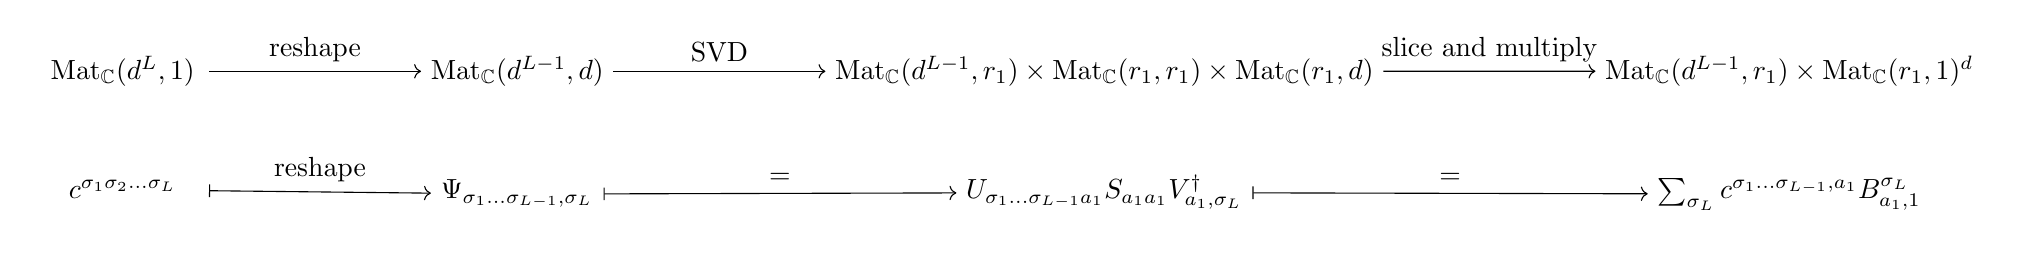
\begin{tikzpicture}
\matrix (m) [matrix of math nodes, row sep=2.55em, column sep=7.7em, minimum width=6.2em]
{
	\text{Mat}_{\mathbb{C}}( d^{L}, 1 ) & \text{Mat}_{\mathbb{C}}(d^{L-1}, d ) & \text{Mat}_{\mathbb{C}}(d^{L-1},r_1 ) \times \text{Mat}_{\mathbb{C}}(r_1, r_1) \times \text{Mat}_{\mathbb{C}}(r_1 , d) & \text{Mat}_{\mathbb{C}}(d^{L-1}, r_1) \times \text{Mat}_{\mathbb{C}}(r_1, 1)^d \\
	c^{\sigma_1 \sigma_{2} \dots \sigma_L} & \Psi_{\sigma_1 \dots  \sigma_{L-1}, \sigma_L } &  U_{ \sigma_1 \dots \sigma_{L-1} a_1 } S_{a_1 a_1} V^{\dagger}_{a_1, \sigma_{L} } & \sum_{\sigma_L} c^{\sigma_{1} \dots \sigma_{L-1}, a_1 } B^{\sigma_L}_{a_{1}, 1}\\
};
\path[->]
(m-1-1) edge node [above] { \text{reshape} } (m-1-2)
(m-1-2) edge node [above] { \text{SVD} } (m-1-3)
(m-1-3) edge node [above] { \text{slice and multiply} } (m-1-4)
;
\path[|->]
(m-2-1) edge node [above] { \text{reshape} } (m-2-2)
(m-2-2) edge node [above] { = } (m-2-3)
(m-2-3) edge node [above] { = } (m-2-4)
;
\end{tikzpicture}  
\]


\[
\begin{gathered}
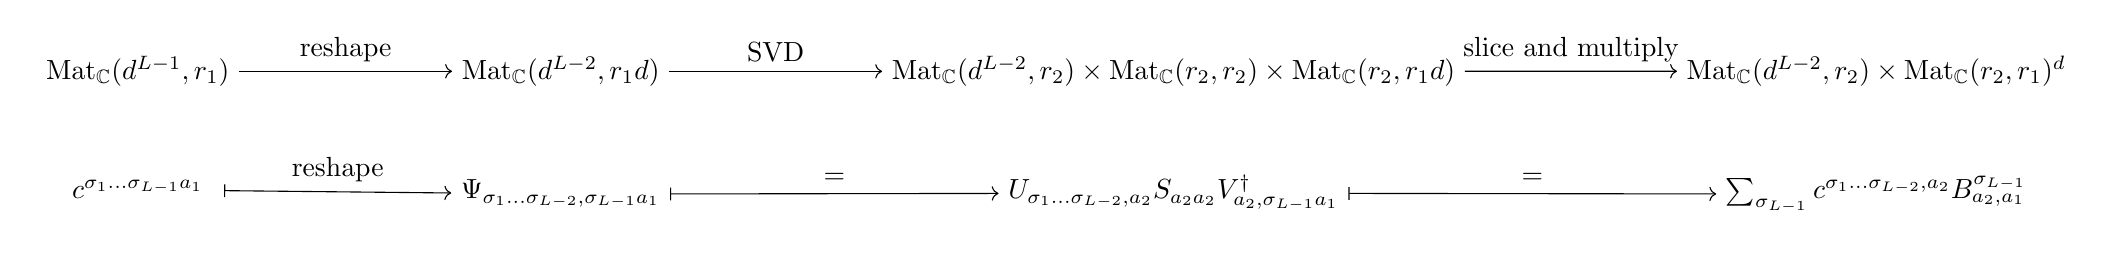
\begin{tikzpicture}
\matrix (m) [matrix of math nodes, row sep=2.55em, column sep=7.7em, minimum width=6.2em]
{
	\text{Mat}_{\mathbb{C}}( d^{L-1}, r_1 ) & \text{Mat}_{\mathbb{C}}(d^{L-2}, r_1d ) & \text{Mat}_{\mathbb{C}}(d^{L-2},r_2 ) \times \text{Mat}_{\mathbb{C}}(r_2, r_2) \times \text{Mat}_{\mathbb{C}}(r_2 , r_1d) & \text{Mat}_{\mathbb{C}}(d^{L-2}, r_2) \times \text{Mat}_{\mathbb{C}}(r_2, r_1)^d \\
	c^{\sigma_1  \dots \sigma_{L-1} a_1} & \Psi_{\sigma_1 \dots \sigma_{L-2}, \sigma_{L-1} a_1 } &  U_{ \sigma_1 \dots \sigma_{L-2}, a_2 } S_{a_2 a_2} V^{\dagger}_{a_2, \sigma_{L-1} a_1 } & \sum_{\sigma_{L-1}} c^{\sigma_{1} \dots \sigma_{L-2}, a_2 } B^{\sigma_{L-1}}_{a_{2}, a_1} \\
};
\path[->]
(m-1-1) edge node [above] { \text{reshape} } (m-1-2)
(m-1-2) edge node [above] { \text{SVD} } (m-1-3)
(m-1-3) edge node [above] { \text{slice and multiply} } (m-1-4)
;
\path[|->]
(m-2-1) edge node [above] { \text{reshape} } (m-2-2)
(m-2-2) edge node [above] { = } (m-2-3)
(m-2-3) edge node [above] { = } (m-2-4)
;
\end{tikzpicture}   \\
\vdots
\end{gathered}
\]

\begin{equation}\label{Eq:RightMPSoperation}
\begin{gathered}
\begin{tikzpicture}[framed]
\matrix (m) [matrix of math nodes, row sep=2.55em, column sep=7.7em, minimum width=6.2em]
{
	\text{Mat}_{\mathbb{C}}( d^{L-(i-1)}, r_{i-1} ) & \text{Mat}_{\mathbb{C}}(d^{L-i}, r_{i-1}d ) & \text{Mat}_{\mathbb{C}}(d^{L-i},r_i ) \times \text{Mat}_{\mathbb{C}}(r_i, r_i) \times \text{Mat}_{\mathbb{C}}(r_i , r_{i-1}d) & \text{Mat}_{\mathbb{C}}(d^{L-i}, r_i) \times \text{Mat}_{\mathbb{C}}(r_i, r_{i-1})^d \\
	c^{\sigma_1  \dots \sigma_{L-(i-1)} a_{i-1}} & \Psi_{\sigma_1 \dots \sigma_{L-i}, \sigma_{L-(i-1)} a_{i-1 } } &  U_{ \sigma_1 \dots \sigma_{L-i}, a_i } S_{a_i a_i} V^{\dagger}_{a_i, \sigma_{L-(i-1)} a_{i-1} } & \sum_{\sigma_{L-(i-1)}} c^{\sigma_{1} \dots \sigma_{L-i}, a_i } B^{\sigma_{L-(i-1)}}_{a_{i}, a_{i-1}} \\
};
\path[->]
(m-1-1) edge node [above] { \text{reshape} } (m-1-2)
(m-1-2) edge node [above] { \text{SVD} } (m-1-3)
(m-1-3) edge node [above] { \text{slice and multiply} } (m-1-4)
;
\path[|->]
(m-2-1) edge node [above] { \text{reshape} } (m-2-2)
(m-2-2) edge node [above] { = } (m-2-3)
(m-2-3) edge node [above] { = } (m-2-4)
;
\end{tikzpicture}   
\end{gathered}
\end{equation}

Remember that $r_i \leq \min{(d^{L-i}, r_{i-1} d)} $ and for $i=L$, just do reshape and slice and multiply operations.

Then, finally, the \textbf{right normalization} is derived and is such:
\[
	\begin{gathered}
	V^{\dagger}V = 1 \Longrightarrow \\
	(V^{\dagger}V)_{a_i a'_i} = \delta_{a_i a'_i} = V^{\dagger}_{a_i, \sigma_{L-(i-1)}a_{i-1}} V_{\sigma_{L-(i-1)}a_{i-1}, a_i'} = B^{\sigma_{L - (i-1)}}_{a_i, a_{i-1}} (V^{\dagger})^{\dagger}_{ \sigma_{L - (i-1)}a_{i-1}, a_i' } = \\
	= B^{\sigma_{L- (i-1)}}_{ a_i a_{i-1}} (V^{\dagger})^*_{a_i', \sigma_{L- (i-1)}, a_{i-1}} = B^{\sigma_{L-(i-1)}}_{ a_i, a_{i-1}} B^{\sigma_{L - (i-1)}}_{a_i' , a_{i-1}} = B^{\sigma_{L-(i-1)}}_{a_i a_{i-1}} (B^{\dagger})^{\sigma_{L-(i-1)}}_{ a_{i-1} a_i'} \qquad \, \forall i = 1 \dots L
	\end{gathered}
\]

\begin{equation}
\Longrightarrow \sum_{ \sigma_{L-(i-1)}} B^{\sigma_{L-(i-1)}} (B^{\dagger})^{\sigma_{L-(i-1)}} = 1
\end{equation}



\begin{multicols*}{2}





cf. Sec. 4, Matrix Product States (MPS) of Schollw\"{o}ck \cite{Scho2010}.  

Necessarily, given matrix $M\in \text{Mat}_{\mathbb{K}}(M,N)$ (notation in Bridgeman and Chubb (2017) \cite{BrCh2017} and \href{http://docs.nvidia.com/cuda/cusolver/index.html}{CUDA Toolkit Documentation}; I will follow the notation in Schollw\"{o}ck \cite{Scho2010} since his $A$,$B$ denote specific physical meaning).  

For 
\[
U\in \text{Mat}_{\mathbb{K}}(N_A, \min{(N_A,N_B)}) \text{ s.t. } UU^{\dag}=1
\]
\[
S \in \text{Mat}_{\mathbb{K}}(\min{(N_A,N_B)}, \min{(N_A,N_B)} )
\]
s.t. $S$ diagonal with nonnegative $S_{aa} = s_a$, i.e. $S_{ij} = \delta_{ij}s_i$ s.t. $s_i\geq 0$ \, $\forall \, i = 1,2, \dots \min{(N_A,N_B)}$.  

$r\equiv $ (Schmidt) rank of $M :=$ number of nonzero singular values.  

Assume $s_1\geq s_2 \geq \dots \geq s_r \geq 0$.  

$V^{\dag} \in \text{Mat}_{\mathbb{K}}(\min{(N_A,N_B)},N_B)$ s.t. $V^{\dag}V=1$.  

\begin{tikzpicture}
  \matrix (m) [matrix of math nodes, row sep=1.75em, column sep=4.8em, minimum width=1.2em]
  {
	\text{Mat}_{\mathbb{K}}(N_A,N_B) & U_{\mathbb{K}}(N_A,\min{(N_A,N_B)}) \times \text{diag}_{\mathbb{K}}(\min{(N_A,N_B)}) \times U_{\mathbb{K}}(\min{(N_A,N_B)},N_B) \\ 
    M &  USV^{\dag} \\
};
  \path[->]
  (m-1-1) edge node [above] { SVD } (m-1-2)
  ;
  \path[|->]
  (m-2-1) edge node [above] {  SVD } (m-2-2)
  ;
\end{tikzpicture}  

Optimal approximation of $M$ (rank $r$ by matrix $M'$ (rank $r' <r$) property.  

In Frobenius norm $\| M \|_F^2 := \sum_{i,j} |M_{ij}|^2$, induced by inner product $\langle M | N \rangle =\text{tr}M^{\dag}N$.  Indeed, 
\[
\text{tr}M^{\dag}N = (M^{\dag})_{ik} N_{ki} = \overline{M}_{ki} N_{ki}
\]
and so for 
\begin{equation}
M'=US'V^{\dag}, \qquad \, S'=\text{diag}(s_1,s_2 \dots s_{r'}, 0 \dots ) \qquad \,
\end{equation}
cf. Eq. (19) of Schollw\"{o}ck \cite{Scho2010}, i.e. 1 sets all but 1st $r'$ singualr values to $0$.  

Use singular value decomposition (SVD) to derive Schmidt decomposition of general quantum state. 

$\forall \, $ pure state $|\psi \rangle$ on $AB$, 
\[
|\psi \rangle = \sum_{i,j} \Psi_{ij}|i\rangle_A |j\rangle_B
\]
where $\lbrace |i\rangle_A \rbrace, \lbrace |j\rangle_B \rbrace$ orthonormal bases of $A,B$ ((complex) Hilbert spaces), with dim. $N_A,N_B$, respectively.  

Let $\Psi_{i,j} \in \text{Mat}_{\mathbb{K}}(N_A,N_B)$.  

Then \textbf{reduced density operators} $\widehat{\rho}_A,\widehat{\rho}_B$ are such that 
\[
\begin{gathered}
\begin{aligned} 
	& \widehat{\rho}_A = \text{tr}_B|\psi \rangle \langle \psi | \\ 
	& \widehat{\rho}_B = \text{tr}_A|\psi \rangle \langle \psi | \\ 
\end{aligned}
\end{gathered}
\]
In matrix form, 
\[
\begin{aligned}
	& \rho_A = \Psi \Psi^{\dag} \\ 
	& \rho_B = \Psi^{\dag} \Psi 
\end{aligned}
\]
Indeed, 
\[
\begin{gathered}
\begin{aligned} 
	& (\rho_A)_{ij} = \Psi_{ik} \overline{\Psi}_{jk} \\
	& (\rho_B)_{ij} = \overline{\Psi}_{ki}  \Psi_{kj} \end{aligned} \\
\begin{gathered}
|\psi \rangle \langle \psi | = \sum_{i,j} \Psi_{ij} |i\rangle_A |j\rangle_B \sum_{l,m} \overline{\Psi}_{lm}\langle l |_A \langle m |_B \\
\text{tr}_B|\psi \rangle \langle \psi | = \sum_{i,j} \Psi_{ik} \overline{\Psi}_{jk} |i \rangle_A \rangle j |_A
\end{gathered}
\end{gathered}
\]
In matrix form, 
\[
\begin{aligned}
	& \rho_A = \Psi \Psi^{\dag} \\ 
	&  \rho_B = \Psi^{\dag} \Psi
\end{aligned}
\]
Carry out SVD on $\Psi$ in Eq. (20) of Schollw\"{o}ck \cite{Scho2010}, 
\[
|\psi \rangle = \sum_{i,j} \Psi_{ij} |i\rangle_A |j\rangle_B
\]
\[
\begin{gathered}
|\psi \rangle = \sum_{ij} \Psi_{ij} | i \rangle_A |j \rangle_B = \sum_{ij} \sum_{a=1}^{\min{(N_A,N_B)}} U_{ia} S_{aa} \overline{V}_{ja} |i \rangle_A | j \rangle_B = \sum_{a=1}^{ \min{(N_A,N_B)}} \sum_i U_{ia} | i \rangle_A s_a \sum_j \overline{V}_{ja} | j \rangle_B = \sum_{a=1}^{ \min{ (N_A,N_B)} } s_a |a \rangle_A |a\rangle_B
\end{gathered}
\]
Due to orthogonality of $U,V^{\dag}$, $\lbrace |a \rangle_A \rangle, \lbrace | a \rangle_B \rbrace$ orthonormal, and can be extended to be orthonormal bases of $A,B$.  

If we restrict the sum to run only over the $r\leq \min{(N_A,N_B)}$ positive nonzero singular values (i.e., for $\sum_{a=1}^{\min{(N_A,N_B)}}$, $_a>0$ \, $\forall \, a \leq r$, and so 
\[
|\psi \rangle =\sum_{a=1}^r s_a |a\rangle_A |a\rangle_B
\]
$r=1$ (classical) product states.  $|\psi \rangle = s_1 |1\rangle_A |1\rangle_B$.  \\
$r>1$ entangled (quantum) states.  

Schmidt decomposition on reduced density operators for $A$ and $B$:  

\[
\begin{aligned}
	& \widehat{\rho}_A =\sum_{a=1}^r s_a^2 |a\rangle_A \langle a |_A \\ 
	& \widehat{\rho}_B = \sum_{a=1}^r s_a^2 |a\rangle_B \langle a |_B
\end{aligned}
\]
Respective eigenvectors are left and right singular vectors.  

Von Neumann entropy can be read off:  
\[
S_{A|B}(|\psi \rangle) = -\text{tr}\widehat{\rho}_A \log_2{\widehat{\rho}_A} = -\sum_{a=1}^r s_a^2 \log_2{s_a^2}
\]

In view of large size of Hilbert spaces, approximate $| \psi \rangle$ by some $| \widetilde{\psi} \rangle$ spanned over state spaces $A,B$ that have dims. $r'$ only.  

Since 2-norm of $| \psi \rangle$, 
\[
\| | \psi\rangle \|_2^2 = \sum_{ij} |\Psi_{ij} |^2 = \| \Psi \|^2_F
\]
since
\[
\| | \psi\rangle \|_2^2 = \sum_{a=1}^r s_a^2 = \sum_{ij} |\Psi_{ij} |^2
\] 
iff $\lbrace |i \rangle \rbrace , \lbrace | j  \rangle \rbrace$ orthonormal.  Optimal approx. of 2-norm given by optimal approx. of $\Psi$ by $\overline{\Psi}$ in Frobenius norm, where $\overline{\Psi}$ is matrix of rank $r'$.  

$\overline{\Psi} = US'V^{\dag}$, $S' =\text{diag}(s_1 , \dots s_{r'} , 0\dots )$ from above. 

$\Longrightarrow $ Schmidt decomposition of approximate state 
\begin{equation}
| \overline{\Psi}\rangle = \sum_{a=1}^{r'} s_a|a\rangle_A | a \rangle_B
\end{equation}
cf. Eq. (27) of  Schollw\"{o}ck \cite{Scho2010}, where $s_a$ must be rescaled if normalization desired.  

\subsection{QR decomposition}
cf. 4.1.2. of  Schollw\"{o}ck \cite{Scho2010}.  

If actual value of singular values not used explicitly, then use \emph{QR decomposition}.  

QR decomposition: $\forall \, M \in \text{Mat}_{\mathbb{K}}(N_A,N_B)$, 
\begin{equation}
M=QR, \, Q\in U_{\mathbb{K}}(N_A), \text{ i.e. } Q^{\dag}Q = 1=QQ^{\dag} , \, R \in \text{Mat}_{\mathbb{K}}(N_A,N_B) \text{ s.t. } \text{ upper triangular, i.e. } R_{ij}= 0 \text{ if } i >j 
\end{equation}
\textbf{thin} QR decomposition: assume $N_A>N_B$.  Then bottom $N_A-N_B$ rows of $R$ are $0$, so 
\[
\begin{gathered}
M=Q \left[ \begin{matrix} R_1 \\ 0 \end{matrix} \right] = \left[ \begin{matrix} Q_1 & Q_2 \end{matrix} \right] \left[ \begin{matrix} R_1 \\ 0 \end{matrix} \right] = Q_1R_1 \\
\begin{aligned}
& Q_1 \in \text{Mat}_{\mathbb{K}}(N_A,N_B) \\ 
& R_1 \in \text{Mat}_{\mathbb{K}}(N_B,N_B) 
\end{aligned}
\end{gathered}
\]
While $Q_1^{\dag}Q_1=1$ in general $Q_1 Q_1^{\dag} \neq 1$

\section{Matrix Product States (MPS)}

cf. Section 4.13 Decomposition of arbitrary quantum states into MPS of  Schollw\"{o}ck \cite{Scho2010}.  

Consider lattice of $L$ sites, $d$-dim. local state spaces $\lbrace \sigma_i \rbrace_{i=1,\dots L}$.  

Most general pure quantum state on lattice (assume normalized) 
\begin{equation}
|\psi \rangle = \sum_{\sigma_1 \dots \sigma_L} c_{\sigma_1 \dots \sigma_L }|\sigma_1 \dots \sigma_L \rangle
\end{equation}
cf. Eq. (30) of  Schollw\"{o}ck \cite{Scho2010},

\subsection{Left-canonical matrix product state}  
cf.  Schollw\"{o}ck \cite{Scho2010},

Consider the process of refactoring or "flattening", which I claim to be a functor \emph{flatten}: 
\[
| \psi \rangle \in \mathcal{H} \text{ s.t. } \text{dim}\mathcal{H} = d^L \mapsto \Psi \in \text{Mat}_{\mathbb{K}}(d,d^{L-1})
\]
\[
\Psi_{\sigma_1, (\sigma_2 \dots \sigma_L) } = c_{\sigma_1 \dots \sigma_L}
\]
\begin{equation}
\begin{gathered}
\xrightarrow{ \text{ SVD } } c_{\sigma_1 \dots \sigma_L} = \Psi_{\sigma_1, (\sigma_2 \dots \sigma_L)} = \sum_a^{r_1} U_{\sigma_1, a_1} S_{a_1,a_1} (V^{\dag})_{a_1, (\sigma_2 \dots \sigma_L)} \equiv \sum_{a_1}^{r_1} U_{\sigma_1 , a_1} c_{a_1 , \sigma_2 \dots \sigma_L}
\end{gathered}
\end{equation}
i.e.
\[
\begin{aligned}
	& (\mathbb{K}^d)^L \to \text{Mat}_{\mathbb{K}}(1,r) \times \text{Mat}_{\mathbb{K}}(r_1 d, d^{L-2}) \\ 
	& c_{\sigma_1 \dots \sigma_L} \mapsto A_{a_1}^{\sigma_1} , \Psi_{(a_1\sigma_2), (\sigma_3\dots \sigma_L)} 
\end{aligned}
\]
s.t. 
\[
c_{\sigma_1\dots \sigma_L} = \sum_{a_1}^{r_1} A_{a_1}^{\sigma_1} \Psi_{(a_1\sigma_2), (\sigma_3 \dots \sigma_L)}
\]
where rank $r_1 \leq d$.  
\[
U \in \text{Mat}_{\mathbb{K}}(d,\min{(d,r)}) = \text{Mat}_{\mathbb{K}}(d,r)
\]
Consider $d$ row vectors $A^{\sigma_1}$, $A^{\sigma_1}_{a_1} = U_{\sigma_1,a_1}$.  

\[
\begin{gathered}
c_{a_1\sigma_2 \dots \sigma_L } = \sum_{a_1}^{r_1} A_{a_1}^{\sigma_1} \Psi_{(a_1,\sigma_2),(\sigma_3\dots \sigma_L)} \text{ with } \\
\Psi_{(a_1\sigma_2),(\sigma_3\dots \sigma_L)}\in \text{Mat}_{\mathbb{K}}(r_1d,d^{L-2})
\end{gathered}
\]
So from Eq. (34) of  Schollw\"{o}ck \cite{Scho2010},
\begin{equation}
\begin{gathered}
	c_{\sigma_1 \dots \sigma_L} = \sum_{a_1}^{r_1} \sum_{a_2}^{r_2} A_{a_1}^{\sigma_1} U_{ (a_1\sigma_2) , a_2} S_{a_2,a_2} (V^{\dag})_{a_2, (\sigma_3\dots \sigma_L)} = \sum_{a_1}^{r_1} \sum_{a_2}^{r_2} A_{a_1}^{\sigma_1} A_{a_1,a_2}^{\sigma_2} \Psi_{(a_2\sigma_3), (\sigma_4\dots \sigma_L)}
\end{gathered}
\end{equation}
So for 
\[
U\in \text{Mat}_{\mathbb{K}}(d,r_1\times r_2) \mapsto \lbrace A^{\sigma_2} \rbrace_{\sigma_2}, \qquad \, | \lbrace A^{\sigma_2} \rbrace_{\sigma_2} | = d , \qquad \, A^{\sigma_2} \in \text{Mat}_{\mathbb{K}}(r_1,r_2)
\]
$A^{\sigma_2}_{a_1,a_2} = U_{(a_1,\sigma_2),a_2}$ and multiplied $S$ and $V^{\dag}$, 
\[
SV^{\dag} \mapsto \Psi \in \text{Mat}_{\mathbb{K}}(r_2d, d^{L-3}); \qquad \, r_2 \leq r_1 d \leq d^2
\]
and so continuing the application of SVD and refactoring (what I call applying the \emph{flatten} functor)
\[
\begin{gathered}
\xrightarrow{ \text{ SVD } } c_{\sigma_1 \dots \sigma_L} = \sum_{a_1 \dots a_{L-1}} A^{\sigma_1}_{a_1} A^{\sigma_2}_{a_1 a_2} \dots A^{\sigma_{L-1}}_{a_{L-2}, a_{L-1} } A^{\sigma_L }_{a_L-1 } \equiv A^{\sigma_1} A^{\sigma_2} \dots A^{\sigma_{L-1}} A^{\sigma_L}
\end{gathered}
\]

\subsubsection{Matrix Product State (definition)}

\begin{definition}[Matrix Product State]
\begin{equation}
|\psi \rangle = \sum_{\sigma_1 \dots \sigma_L} A^{\sigma_1}A^{\sigma_2} \dots A^{\sigma_{L-1}} A^{\sigma_L} | \sigma_1 \dots \sigma_L \rangle
\end{equation}
\end{definition}

Maximally, the dims. are 
\[
(1\times d), (d\times d^2) \dots (d^{L/2-1} \times d^{L/2} ), (d^{L/2} \times d^{L/2-1} ) \dots (d^2 \times d), (d\times 1)
\]
Since $\forall \, $ SVD, $U^{\dag} U=1$, 
\[
\delta_{a_l , a_l'} = \sum_{a_{l-1} a_l} (U^{\dag})_{a_l,(a_{l-1} \sigma_l)} U_{(a_{l-1} \sigma_l),a'_l } = \sum_{a_{l-1} \sigma_l} (A^{\sigma_l})^{\dag}_{a_l,a_{l-1}} A^{\sigma_l}_{a_{l-1},a_l'} = \sum_{\sigma_l} ( (A^{\sigma_2})^{\dag} A^{\sigma_l} )_{a_l,a_l'}
\]
or 
\begin{equation}
	\sum_{\sigma_l} (A^{\sigma_l})^{\dag} A^{\sigma_l} = 1
\end{equation}
cf. Eq. (38) of  Schollw\"{o}ck \cite{Scho2010},

If for $\lbrace A^{\sigma_l} \rbrace_{\sigma_l} $, $\sum_{\sigma_l} (A^{\sigma_l})^{\dag} A = 1$, $\lbrace A^{\sigma_l} \rbrace_{\sigma_l}$ are \textbf{left-normalized}; matrix product states that consist of only left-normalized matrices are \textbf{left-canonical}.  

View Density Matrix Renormalization Group (DMRG) decomposition of universe into blocks $A$ and $B$, split lattice into parts $A$,$B$, where $A$ compries sites $1$ through $l$ and $B$ sites $l+1$ through $L$.  

\[
\begin{aligned}
	& | a_l \rangle_A = \sum_{\sigma_1 \dots \sigma_l} (A^{\sigma_1} A^{\sigma_2} \dots A^{\sigma_l} )_{a_l,1} | \sigma_1 \dots \sigma_l \rangle \\ 
		& | a_l \rangle_B = \sum_{\sigma_{l+1} \dots \sigma_L} (A^{\sigma_{l+1}} A^{\sigma_{l+2}} \dots A^{\sigma_L} )_{a_l,1} | \sigma_{l+1} \dots \sigma_L \rangle 
\end{aligned}
\]
s.t. matrix product state (MPS) is 
\[
|\psi \rangle =\sum_{a_l} | a_l \rangle_A | a_l \rangle_B
\]

\subsubsection{Summarize this procedure of constructing, from a pure state, the matrix product state (version) by successive application Singular Value Decomposition (SVD) from the Category Theory point of view}

Consider all applications of SVD to get to a matrix product state (MPS): 
\begin{tikzpicture}
  \matrix (m) [matrix of math nodes, row sep=1.75em, column sep=4.8em, minimum width=1.2em]
  {
	(\mathbb{K}^d)^L & (\text{Mat}_{\mathbb{K}}(1,r_1))^d \times (\text{Mat}_{\mathbb{K}}(r_1,r_2))^d \times \dots \times (\text{Mat}_{\mathbb{K}}(r_{L-2},r_{L-1}))^d \times (\text{Mat}_{\mathbb{K}}(r_{L-1},1))^d \\
    c_{\sigma_1 \dots \sigma_L}  &  c_{\sigma_1\dots \sigma_L} = \sum_{a_1 \dots a_{L-1}} A^{\sigma_1}_{a_1} A_{a_1a_2}^{\sigma_2} \dots A^{\sigma_{L-1}}_{a_{L-2}, a_{L-1}} A_{a_{L-1}}^{\sigma_L} \\
};
  \path[->]
  (m-1-1) edge node [above] { SVD } (m-1-2)
  ;
  \path[|->]
  (m-2-1) edge node [above] {  SVD } (m-2-2)
  ;
\end{tikzpicture}  
and remember the maximal values that the $r_i$'s can take:
\[
\begin{gathered}
	\begin{aligned}
& r_1 \leq d \\ 
	& r_2 \leq d^2 
\end{aligned}	 \qquad \, 	\begin{aligned}
& r_{L/2} \leq d^{L/2} \\ 
	& r_{L/2+1} \leq d^{L/2-1} 
\end{aligned} \qquad \, 	\begin{aligned}
& r_{L-2} \leq d^2 \\ 
	& r_{L-1} \leq d 
\end{aligned}
\end{gathered}
\]

Let us explicitly note the functors (that were applied) flatten (and its inverse), and the application of SVD, explicitly:

\end{multicols*}
%\begin{multicols*}{1}

\[
\begin{tikzpicture}
  \matrix (m) [matrix of math nodes, row sep=1.75em, column sep=2.8em, minimum width=1.2em]
  {
	(\mathbb{K}^d)^L & \text{Mat}_{\mathbb{K}}(d,d^{L-1})  & U_{\mathbb{K}}(d,r_1) \times \text{diag}_{\mathbb{K}}(r_1) \times U_{\mathbb{K}}(r_1,d^{L-1}) &  (\text{Mat}_{\mathbb{K}}(1,r_1))^d \times \text{Mat}_{\mathbb{K}}(r_1d, d^{L-2}) &   (\text{Mat}_{\mathbb{K}}(1,r_1))^d \times (\mathbb{K}^{r_1}) \times (\mathbb{K}^d)^{L-1}  
 \\
	    c_{\sigma_1 \dots \sigma_L} & c_{\sigma_1 \dots \sigma_L} = \Psi_{\sigma_1,(\sigma_2\dots \sigma_L)} & \Psi_{\sigma_1,(\sigma_2\dots \sigma_L)} = \sum_{a_1}^{r_1}U_{\sigma_1a_1} S_{a_1,a_1} (V^{\dag})_{a_1,(\sigma_2 \dots \sigma_L)} & c_{a_1\sigma_2\dots \sigma_L} = \sum_{a_1}^{r_1} A_{a_1}^{\sigma_1} \Psi_{(a_1,a_2),(\sigma_3 \dots \sigma_L)} &  c_{a_1\sigma_2\dots \sigma_L} = \sum_{a_1}^{r_1} A^{\sigma_1}_{a_1} c_{a_1 \sigma_2 \dots \sigma_L} \\
};
  \path[->]
  (m-1-1) edge node [above] { $\text{flatten}^{-1}$ } (m-1-2)
  (m-1-2) edge node [above] { SVD } (m-1-3)
  (m-1-3) edge node [above] { $\cong$ } (m-1-4)
  (m-1-4) edge node [above] { flatten } (m-1-5)
  ;
  \path[|->]
  (m-2-1) edge node [above] { $\text{flatten}^{-1}$ } (m-2-2)
  (m-2-2) edge node [above] { SVD } (m-2-3)
  (m-2-3) edge node [above] { $\cong$ } (m-2-4)
  (m-2-4) edge node [above] { flatten } (m-2-5)
  ;
\end{tikzpicture}  
\]
with $\cong$ in this case denoting an isomorphism (clearly).  


In considering some kind of recursive algorithm, so to repeat some series of steps until a matrix product state is obtained, consider this:
\[
\begin{tikzpicture}
  \matrix (m) [matrix of math nodes, row sep=1.75em, column sep=4.8em, minimum width=1.2em]
  {
	(\mathbb{K}^d)^L & (\text{Mat}_{\mathbb{K}}(1,r_1))^d \times \mathbb{K}^{r_1} \times (\mathbb{K}^d)^{L-1} \\
    c_{\sigma_1 \dots \sigma_L}  &  c_{\sigma_1\dots \sigma_L} = \sum_{a_1}^{r_1} A^{\sigma_1}_{a_1} c_{a_1 \sigma_2\dots \sigma_L} \\ 
};
  \path[->]
  (m-1-1) edge node [above] {  } (m-1-2)
  ;
  \path[|->]
  (m-2-1) edge node [above] {  } (m-2-2)
  ;
\end{tikzpicture}  
\]

So in summary, to obtain matrix product states, starting from a matrix, 
\begin{equation}
\begin{tikzpicture}[framed]
  \matrix (m) [matrix of math nodes, row sep=1.55em, column sep=1.7em, minimum width=1.2em]
  {
	\text{Mat}_{\mathbb{K}}(d,d^{L-1})  & (\text{Mat}_{\mathbb{K}}(1,r_1))^d \times \text{Mat}_{\mathbb{K}}(r_1d, d^{L-2}) & \dots &   (\text{Mat}_{\mathbb{K}}(1,r_1))^d \times (\text{Mat}_{\mathbb{K}}(r_1,r_2))^d \times \dots \times (\text{Mat}_{\mathbb{K}}(r_{n-1},r_{n}))^d \times (\text{Mat}_{\mathbb{K}}(r_{n}d,d^{L-(n+1)}))^d    \\
    \Psi_{\sigma_1,(\sigma_2\dots \sigma_L)} &   \sum_{a_1}^{r_1} A_{a_1}^{\sigma_1} \Psi_{(a_1,\sigma_2),(\sigma_3 \dots \sigma_L)}  & \dots & \sum_{a_1,a_2,\dots a_n}^{r_1,r_2,\dots r_n} A^{\sigma_1}_{a_1} A^{\sigma_2}_{a_1a_2}\dots A^{\sigma_n}_{a_{n-1}a_n} \Psi_{ (a_n \sigma_{n+1}), (\sigma_{n+2}\dots \sigma_L) } \\ 
};
  \path[->]
  (m-1-1) edge node [above] {  } (m-1-2)
  (m-1-2) edge node [above] {  } (m-1-3)
  (m-1-3) edge node [above] {  } (m-1-4)
  ;
  \path[|->]
  (m-2-1) edge node [above] {  } (m-2-2)
  (m-2-2) edge node [above] {  } (m-2-3)
  (m-2-3) edge node [above] {  } (m-2-4)
;
\end{tikzpicture}  
\end{equation}



%\end{multicols*}
%\begin{multicols*}{2}

\subsection{Right-canonical matrix product state}  
cf.  Schollw\"{o}ck \cite{Scho2010},

We can start from right in order to obtain 
\[
\begin{gathered}
	c_{\sigma_1\dots \sigma_L} = \Psi_{(\sigma_1 \dots \sigma_{L-1}), \sigma_L } = \sum_{a_{L-1}} U_{(\sigma_1 \dots \sigma_{L-1} ), a_{L-1} } S_{a_{L-1}, a_{L-1} } (V^{\dag})_{a_{L-1}, \sigma_L } = \sum_{a_{L-1}} \Psi_{(\sigma_1\dots \sigma_{L-2}), (\sigma_{L-1} a_{L-1} ) } B^{\sigma_L}_{a_{L-1}} = \\ 
 = \sum_{a_{L-1},a_{L-2}} U_{(\sigma_1 \dots \sigma_{L-2} ), a_{L-2} } S_{a_{L-2}, a_{L-2} } (V^{\dag})_{a_{L-2}, (\sigma_{L-1}a_{L-1}) } B^{\sigma_L}_{a_{L-1}}  = \sum_{a_{L-2},a_{L-1}} \Psi_{(\sigma_1\dots \sigma_{L-3}), (\sigma_{L-2} a_{L-2} ) } B^{\sigma_{L-1}}_{a_{L-2},a_{L-1}} B^{\sigma_L}_{a_{L-1}} = \dots \\ 
\end{gathered}
\]
or consider 
\[
\begin{tikzpicture}
  \matrix (m) [matrix of math nodes, row sep=1.95em, column sep=3.8em, minimum width=1.8em]
  {
	(\mathbb{K}^d)^L & \text{Mat}_{\mathbb{K}}(d^{L-1},d)  & U_{\mathbb{K}}(d^{L-1},r_{L-1}) \times \text{diag}_{\mathbb{K}}(r_{L-1}) \times U_{\mathbb{K}}(r_{L-1},d ) &  \text{Mat}_{\mathbb{K}}(d^{L-2},d r_{L-1})  \times ( \text{Mat}_{\mathbb{K}}(r_{L-1}, 1))^d &   \qquad \, 
 \\
	    c_{\sigma_1 \dots \sigma_L} & c_{\sigma_1 \dots \sigma_L} = \Psi_{(\sigma_1\dots \sigma_{L-1}),\sigma_L} & c_{\sigma_1 \dots \sigma_L} =  \sum_{a_{L-1}}^{r_{L-1}}U_{(\sigma_1 \dots \sigma_{L-1}), a_{L-1}} S_{a_{L-1},a_{L-1}} (V^{\dag})_{a_{L-1}, \sigma_L} & \begin{gathered}
	U_{(\sigma_1 \dots \sigma_{L-1}), a_{L-1} } S_{a_{L-1}, a_{L-1}} = \Psi_{(\sigma_1\dots \sigma_{L-2}), (\sigma_{L-1} a_{L-1}) } \\ 
(V^{\dag})_{a_{L-1},\sigma_L} = B^{\sigma_L}_{a_{L-1}} \\
c_{\sigma_1\dots \sigma_L} = \sum_{a_{L-1}} \Psi_{(\sigma_1 \dots \sigma_{L-2} ) , (\sigma_{L-1}, a_{L-1})} B_{a_{L-1}}^{\sigma_L} 
\end{gathered}  &  \qquad \,  \\
\qquad \, & U_{\mathbb{K}}(d^{L-2},r_{L-2}) \times \text{diag}_{\mathbb{K}}(r_{L-2}) \times U_{\mathbb{K}}(r_{L-2},dr_{L-1} ) \times  ( \text{Mat}_{\mathbb{K}}(r_{L-1}, 1))^d  & \text{Mat}_{\mathbb{K}}(d^{L-3},d r_{L-2})   \times  ( \text{Mat}_{\mathbb{K}}(r_{L-2}, r_{L-1}))^d  \times  ( \text{Mat}_{\mathbb{K}}(r_{L-1}, 1))^d &  &  \\
\qquad \,  & c_{\sigma_1\dots \sigma_L} = \sum_{a_{L-1},a_{L-2}} U_{(\sigma_1 \dots \sigma_{L-2} ), a_{L-2} } S_{a_{L-2}, a_{L-2} } (V^{\dag})_{a_{L-2}, (\sigma_{L-1}a_{L-1}) } B^{\sigma_L}_{a_{L-1}} &   \begin{gathered}
	U_{(\sigma_1 \dots \sigma_{L-2}), a_{L-2} } S_{a_{L-2}, a_{L-2}} = \Psi_{(\sigma_1\dots \sigma_{L-3}), (\sigma_{L-2} a_{L-2}) } \\ 
(V^{\dag})_{a_{L-2},(\sigma_{L-1}a_{L-1})} = B^{\sigma_{L-1}}_{a_{L-2}a_{L-1}} \\
c_{\sigma_1\dots \sigma_L} = \sum_{a_{L-1}, a_{L-2}} \Psi_{(\sigma_1 \dots \sigma_{L-3} ) , (\sigma_{L-2}, a_{L-2})} B_{a_{L-2},a_{L-1}}^{\sigma_{L-1}} B^{\sigma_L}_{a_{L-1}} 
\end{gathered}   & &  \\
};
  \path[->]
  (m-1-1) edge node [above] { $\text{flatten}^{-1}$ } (m-1-2)
  (m-1-2) edge node [above] { SVD } (m-1-3)
  (m-1-3) edge node [above] { $\cong$ } (m-1-4)
  (m-1-4) edge node [above] { SVD } (m-1-5)
 (m-3-1) edge node [above] { SVD } (m-3-2)
  (m-3-2) edge node [above] { $\cong$ } (m-3-3)
  ;
  \path[|->]
  (m-2-1) edge node [above] { $\text{flatten}^{-1}$ } (m-2-2)
  (m-2-2) edge node [above] { SVD } (m-2-3)
  (m-2-3) edge node [above] { $\cong$ } (m-2-4)
  (m-2-4) edge node [above] { SVD } (m-2-5)
  (m-4-1) edge node [above] { SVD } (m-4-2)
  (m-4-2) edge node [above] { $\cong$ } (m-4-3)
  ;
\end{tikzpicture}  
\]
with $\cong$ in this case denoting an isomorphism (clearly).  

And so we can explicitly state the recursion step, for the purpose of writing numerical implementations/algorithms: $\forall \, l = 1,2\dots L$,

\begin{tikzpicture}
  \matrix (m) [matrix of math nodes, row sep=1.75em, column sep=4.8em, minimum width=1.2em]
  {
\text{Mat}_{\mathbb{K}}(d^{L-l},d r_{L-(l-1)}) 	 & \text{Mat}_{\mathbb{K}}(d^{L-(l+1)},d r_{L-l}) \times (\text{Mat}_{\mathbb{K}}(r_{L-l},r_{L-(l-1)}))^d \\
    \Psi_{(\sigma_1\dots \sigma_{L-l}), (\sigma_{L-(l-1)} a_{L-(l-1)}) }   &      \Psi_{(\sigma_1\dots \sigma_{L-l}), (\sigma_{L-(l-1)} a_{L-(l-1)}) } = \sum_{a_{L-l}}     \Psi_{(\sigma_1\dots \sigma_{L-(l+1)}), (\sigma_{L-l} a_{L-l}) } B_{a_{L-l},a_{L-(l-1)}}^{\sigma_{L-(l-1)}}  \\ 
};
  \path[->]
  (m-1-1) edge node [above] {  } (m-1-2)
  ;
  \path[|->]
  (m-2-1) edge node [above] {  } (m-2-2)
  ;
\end{tikzpicture}  

and we finally obtained, after successive applications SVD, the matrix product state:

\begin{tikzpicture}
  \matrix (m) [matrix of math nodes, row sep=1.75em, column sep=4.8em, minimum width=1.2em]
  {
(\mathbb{K}^d)^L  & \text{Mat}_{\mathbb{K}}(d^{L-1},d )  & (\text{Mat}_{\mathbb{K}}( 1, r_1))^d \times  (\text{Mat}_{\mathbb{K}}(r_1,r_2))^d \times \dots \times (\text{Mat}_{\mathbb{K}}(r_{L-2},r_{L-1}))^d \times (\text{Mat}_{\mathbb{K}}(r_{L-1}, 1 ))^d \\
    c_{\sigma_1\dots \sigma_L} & \Psi_{(\sigma_1\dots \sigma_{L-l}), \sigma_L }   & c_{\sigma_1\dots \sigma_L} =      \sum_{ a_1 \dots a_{L-1} }  B_{a_1}^{\sigma_1}  B_{a_1a_2}^{\sigma_2 } \dots  B_{a_{L-2}a_{L-1}}^{\sigma_{L-1} }  B_{a_{L-1}}^{\sigma_L} \\ 
};
  \path[->]
  (m-1-1) edge node [above] {  } (m-1-2)
  (m-1-2) edge node [above] {  } (m-1-3)
  ;
  \path[|->]
  (m-2-1) edge node [above] {  } (m-2-2)
  (m-2-2) edge node [above] {  } (m-2-3)
  ;
\end{tikzpicture}  

\begin{multicols*}{2}

Since 
\begin{equation}
V^{\dag} V =1
\end{equation},
then
\begin{equation}
	\delta_{a_l a_l'} = \sum_{\sigma_m a_m } (V^{\dag})_{a_l (\sigma_ma_m) } V_{(\sigma_m a_m) a_l'} = \sum_{\sigma_m a_m } B_{a_l a_m}^{\sigma_m} \overline{B}^{\sigma_m}_{a_l' a_m} \Longrightarrow \sum_{\sigma_m} \boxed{ B^{\sigma_m} (B^{\sigma_m})^{\dag} = 1 }
\end{equation}
The $B$-matrices that obey this condition are referred to as \textbf{right-normalized} matrices.  A matrix product state (MPS) entirely consisting of a product of these right-normalized matrices is called \textbf{right-canonical}.  

\subsection{Matrix Product Operators (MPO)}

The form of a general operator, $\widehat{O}$ is the following:
\begin{equation}
\begin{gathered}
\widehat{O} = \sum_{ \lbrace \sigma \rbrace } \sum_{ \lbrace \sigma' \rbrace } c^{\sigma_1 \dots \sigma_L, \sigma_1' \dots \sigma_L'} | \sigma_1 \dots \sigma_L \rangle \langle \sigma_1' \dots \sigma_L' | \in \mathcal{H} \otimes \mathcal{H}^* 
\end{gathered}
\end{equation}
with $\text{dim}\mathcal{H} = \text{dim}\mathcal{H}^* = d^L$. 

For MPO, do the same decomposition as done in Eq. \ref{Eq:LeftMPSoperation} or in \ref{Eq::RightMPSoperation}, but with the double index $\sigma_i \sigma_i'$ taking the role of index $\sigma_i$ in MPS (i.e. do this substitution and the decomposition will proceed \emph{exactly} as before).

\end{multicols*}
%\begin{multicols*}{1}


\[
\begin{tikzpicture}
\matrix (m) [matrix of math nodes, row sep=2.55em, column sep=7.7em, minimum width=6.2em]
{
	\text{Mat}_{\mathbb{C}}(d^L, d^L)  \\
	\text{Mat}_{\mathbb{C}}(1, (d^2)^{L}) & \text{Mat}_{\mathbb{C}}(d^2, (d^2)^{L-1}) & \text{Mat}_{\mathbb{C}}(d^2, r_i) \times \text{Mat}_{\mathbb{C}}(r_i, r_i) \times \text{Mat}_{\mathbb{C}}(r_i , (d^2)^{L-1}) & \text{Mat}_{\mathbb{C}}(1, r_i)^d \times \text{Mat}_{\mathbb{C}}(r_i, (d^2)^{L-1}) \\
	c^{\sigma_1 \dots \sigma_L, \sigma_1' \dots \sigma_L'}  \\
	c^{\sigma_1 \sigma_1' \sigma_2 \sigma_2' \dots \sigma_L \sigma_L'} & \Psi_{\sigma_1 \sigma_1', (\sigma_{2} \sigma_2', \sigma_{3} \sigma_3' \dots \sigma_L \sigma_L') } &  U_{ \sigma_1\sigma_1', a_1 } S_{a_1 a_1} V^{\dagger}_{a_1, (\sigma_{2} \sigma_2' \dots \sigma_L \sigma_L'} & \sum_{\sigma_1 \sigma_1'} A^{\sigma_1 \sigma_1'}_{1, a_1} c^{a_1, \sigma_{2}\sigma_2' \dots \sigma_L\sigma_L'} \\
};
\path[->]
(m-1-1) edge node [right] { \text{reorder} } (m-2-1)
(m-2-1) edge node [above] { \text{reshape} } (m-2-2)
(m-2-2) edge node [above] { \text{SVD} } (m-2-3)
(m-2-3) edge node [above] { \text{slice and multiply} } (m-2-4)
;
\path[|->]
(m-3-1) edge node [right] { \text{reorder} } (m-4-1)
(m-4-1) edge node [above] { \text{reshape} } (m-4-2)
(m-4-2) edge node [above] { = } (m-4-3)
(m-4-3) edge node [above] { = } (m-4-4)
;
\end{tikzpicture}  
\]

\begin{equation}\label{Eq:LeftMPOoperation}
\begin{tikzpicture}[framed]
\matrix (m) [matrix of math nodes, row sep=2.55em, column sep=7.7em, minimum width=6.2em]
{
	\text{Mat}_{\mathbb{C}}(r_{i-1}, (d^2)^{L-(i-1)}) & \text{Mat}_{\mathbb{C}}(r_{i-1}d^2, (d^2)^{L-i}) & \text{Mat}_{\mathbb{C}}(r_{i-1}d^2, r_i) \times \text{Mat}_{\mathbb{C}}(r_i, r_i) \times \text{Mat}_{\mathbb{C}}(r_i , (d^2)^{L-i}) & \text{Mat}_{\mathbb{C}}(r_{i-1}, r_i)^{d^2} \times \text{Mat}_{\mathbb{C}}(r_i, (d^2)^{L-i}) \\
	c^{a_{i-1}, \sigma_i \sigma_i' \sigma_{i+1} \sigma_{i+1}' \dots \sigma_L \sigma_L'} & \Psi_{a_{i-1}\sigma_i \sigma_i', (\sigma_{i+1}\sigma_{i+1}' \sigma_{i+2}\sigma_{i+2}' \dots \sigma_L\sigma_L') } &  U_{a_{i-1} \sigma_i \sigma_i', a_i } S_{a_i a_i} V^{\dagger}_{a_i, \sigma_{i+1} \sigma_{i+1}' \dots \sigma_L\sigma_L'} & \sum_{\sigma_i \sigma_i'}^{max}A^{\sigma_i \sigma_i'}_{a_{i-1}, a_i} c^{a_i, \sigma_{i+1} \sigma_{i+1}' \dots \sigma_L \sigma_L'} \\
};
\path[->]
(m-1-1) edge node [above] { \text{reshape} } (m-1-2)
(m-1-2) edge node [above] { \text{SVD} } (m-1-3)
(m-1-3) edge node [above] { \text{slice and multiply} } (m-1-4)
;
\path[|->]
(m-2-1) edge node [above] { \text{reshape} } (m-2-2)
(m-2-2) edge node [above] { = } (m-2-3)
(m-2-3) edge node [above] { = } (m-2-4)
;
\end{tikzpicture}  
\end{equation}


\begin{multicols*}{2}


\subsubsection{Numerical implementation; both in BLAS and cuBLAS}

As stated in the \href{http://docs.nvidia.com/cuda/cusolver/index.html#cuds-lt-t-gt-gesvd}{CUDA Toolkit Documentation v8.0} for cuSOLVER, under section 5.3.6. \verb|cusolverDn<t>gesvd()| and Remark 1, \verb|gesvd| "only supports" \verb|m>=n|, for matrix you want to decompose $A\in \text{Mat}_{\mathbb{K}}(m,n)$.  So number of rows must be greater than or equal to number of columns.  And so we can only consider right-normalized matrices in a practical implementation.  

I suspect it's the same in BLAS.  

Consider the very first step, $l=1$, in a procedure to calculate the matrix product state.  

\begin{tikzpicture}
  \matrix (m) [matrix of math nodes, row sep=1.95em, column sep=3.8em, minimum width=1.8em]
  {
	 \text{Mat}_{\mathbb{K}}(d^{L-1},d)  &  U_{\mathbb{K}}(d^{L-1},r_{L-1}) \times \text{diag}_{\mathbb{K}}(r_{L-1}) \times U_{\mathbb{K}}(r_{L-1},d ) &  \text{Mat}_{\mathbb{K}}(d^{L-2},d r_{L-1})  \times ( \text{Mat}_{\mathbb{K}}(r_{L-1}, 1))^d &   \qquad \,  \\	    
 \Psi_{(\sigma_1\dots \sigma_{L-1}),\sigma_L} &  = \sum_{a_{L-1}}^{r_{L-1}}U_{(\sigma_1 \dots \sigma_{L-1}), a_{L-1}} S_{a_{L-1},a_{L-1}} (V^{\dag})_{a_{L-1}, \sigma_L} & \begin{gathered}
	U_{(\sigma_1 \dots \sigma_{L-1}), a_{L-1} } S_{a_{L-1}, a_{L-1}} = \Psi_{(\sigma_1\dots \sigma_{L-2}), (\sigma_{L-1} a_{L-1}) } \\ 
(V^{\dag})_{a_{L-1},\sigma_L} = B^{\sigma_L}_{a_{L-1}} 
\end{gathered} \\
};
  \path[->]
  (m-1-1) edge node [above] { SVD } (m-1-2)
  (m-1-2) edge node [above] { $\cong$ } (m-1-3)
  ;
  \path[|->]
  (m-2-1) edge node [above] { SVD } (m-2-2)
  (m-2-2) edge node [above] { $\cong$ } (m-2-3)
  ;
\end{tikzpicture}  
with $\cong$ in this case denoting an isomorphism, the \emph{reshaping} of a matrix into different matrix size dimensions, which should be the inverse of a "flatten" functor, which I'll denote as $\text{flatten}^{-1}$ as well (and this is this same isomorphism we're talking about).  

Let's deal with the specific procedure of $\text{flatten}^{-1}$, how it reshapes indices in accordance with different matrix size dimensions, and with the so-called "stride" when going from, say, 2-dimensional indices to a "flattened" 1-dimensional index.  

Note also as a practical numerical implementation design point, LAPACK's linear algebra BLAS library package and CUBLAS assumes \emph{column}-major ordering.  

Consider $i= 1,2,\dots L-1$ (for site $i$) (or for $0$-based counting, starting to count from $0$, $i=0,1,\dots L-2$; be aware of this difference as in practical numerical implementation, in C, C++, Python, it assumes $0$-based counting).  

For a state space of dimension $d$, we can consider the specific example of $d=2$, representing say a spin-$1/2$ system.  Then index $\sigma_i$ can be $0$ or $1$: $\sigma_i \in \lbrace 0 ,1\rbrace$.  In general, $\sigma_i \in \lbrace 0 ,1, \dots d-1\rbrace$.  I may use $d$ or $2$ in the context of the number of states (basis vectors) of the spin system (state vector space).  

Consider site $i$.  Suppose the spin system there interacts most with sites $i-1$, $i+1$, and then next sites $i-2$, $i+2$, etc.  So the values at $\sigma_{i-1}, \sigma_{i+1}$, etc. are most important in calculating interactions with spin system at site $i$.  

Then we seek this reshaping of the matrix index - assuming $0$-based counting/ordering, for $l=1$:
\begin{tikzpicture}
  \matrix (m) [matrix of math nodes, row sep=1.95em, column sep=3.8em, minimum width=1.8em]
  {
	\lbrace 0 ,1 \rbrace^{L-1} & \lbrace 0 ,1, \dots 2^{L-1} -1 \rbrace \\
	(\sigma_0,\sigma_1, \dots \sigma_{L-2}) & I_{L-1} := \sigma_0 + 2\sigma_1 + \dots + 2^i \sigma_i + \dots + 2^{L-2}\sigma_{L-2} = \sum_{i=0}^{L-2} 2^i \sigma_i \\
};
  \path[->]
  (m-1-1) edge node [above] { $(\text{flatten})^{-1}$ } (m-1-2)
  ;
  \path[|->]
  (m-2-1) edge node [above] { $(\text{flatten})^{-1}$ } (m-2-2)
  ;
\end{tikzpicture}  

In this way, states of a site $i$ are closest in memory addresses in the allocation of a 1-dim. array, on CPU or GPU memory, so that memory access operations should be efficient.  

Assuming SVD doesn't change the striding, and defining the result of matrix multiplication:
\[
U_{(\sigma_0, \sigma_1 \dots \sigma_{L-2}), a_{L-1} } S_{a_{L-1}, a_{L-1}} =: (US)_{(\sigma_0 \dots \sigma_{L-2} ), a_{L-1} } \in \text{Mat}_{\mathbb{K}}(d^{L-1},r_{L-1} )
\]

We can reshape (i.e. $(\text{flatten})^{-1}$) in such a manner: 
\[
\begin{tikzpicture}
  \matrix (m) [matrix of math nodes, row sep=1.95em, column sep=3.8em, minimum width=1.8em]
  {
	\text{Mat}_{\mathbb{K}}(d^{L-1},r_{L-1})  & \text{Mat}_{\mathbb{K}}(d^{L-2},dr_{L-1}) \\ 
	(US)_{(\sigma_0 \dots \sigma_{L-2} ), a_{L-1} }  & \Psi_{(\sigma_0,\sigma_1 ,\dots \sigma_{L-3}), (\sigma_{L-2} a_{L-1}) }     \\
	\lbrace 0 ,1,\dots 2^{L-1}-1 \rbrace \times \lbrace 0 ,1,\dots r_{L-1} -1 \rbrace & \lbrace 0 ,1,\dots 2^{L-2}-1 \rbrace \times \lbrace 0 ,1,\dots dr_{L-1} -1 \rbrace \\
I_{L-1}, a_{L-1}  & I_{L-1} \mod{ 2^{L-2}} , \frac{ I_{L-1} }{ 2^{L-2} } + da_{L-1} \\
};
  \path[->]
  (m-1-1) edge node [above] { $(\text{flatten})^{-1}$ } (m-1-2)
  (m-3-1) edge node [above] { $(\text{flatten})^{-1}$ } (m-3-2)
  ;
  \path[|->]
  (m-2-1) edge node [above] { $(\text{flatten})^{-1}$ } (m-2-2)
  (m-4-1) edge node [above] { $(\text{flatten})^{-1}$ } (m-4-2)
  ;
\end{tikzpicture}  
\]
Reshaping $V^{\dag}$ at iteration $l=1$ can be done as follows:  
\[
\begin{tikzpicture}
  \matrix (m) [matrix of math nodes, row sep=1.95em, column sep=3.8em, minimum width=1.8em]
  {
	U_{\mathbb{K}}(r_{L-1},d)  & ( \text{Mat}_{\mathbb{K}}( r_{L-1} , 1) )^d \\ 
	(V^{\dag})_{a_{L-1},\sigma_{L-1 } }   & (V^{\dag})_{a_{L-1},\sigma_{L-1} } = B_{a_{L-1}}^{\sigma_{L-1}}     \\
	\lbrace 0 ,1,\dots r_{L-1} -1  \rbrace \times \lbrace 0 ,1,\dots d -1 \rbrace &  (   \lbrace 0 ,1,\dots  r_{L-1}-1 \rbrace )^d \\
a_{L-1}, \sigma_{L-1}  & a_{L-1}  \\
};
  \path[->]
  (m-1-1) edge node [above] { $(\text{flatten})^{-1}$ } (m-1-2)
  (m-3-1) edge node [above] { $(\text{flatten})^{-1}$ } (m-3-2)
  ;
  \path[|->]
  (m-2-1) edge node [above] { $(\text{flatten})^{-1}$ } (m-2-2)
  (m-4-1) edge node [above] { $(\text{flatten})^{-1}$ } (m-4-2)
  ;
\end{tikzpicture}  
\]

Let's do this same procedure, reshaping or $(\text{flatten})^{-1}$, for a general $l$ iteration.  

\[
\begin{tikzpicture}
  \matrix (m) [matrix of math nodes, row sep=1.95em, column sep=3.8em, minimum width=1.8em]
  {
	\text{Mat}_{\mathbb{K}}(d^{L-l},r_{L-l})  & \text{Mat}_{\mathbb{K}}(d^{L-(l+1)},dr_{L-l}) \\ 
	(US)_{(\sigma_0 \dots \sigma_{L-(l+1)} ), a_{L-l } }  & \Psi_{(\sigma_0,\sigma_1 ,\dots \sigma_{L-(l+2)}), (\sigma_{L-(l+1)} a_{L-l}) }     \\
	\lbrace 0 ,1,\dots d^{L-l}-1 \rbrace \times \lbrace 0 ,1,\dots r_{L-l} -1 \rbrace & \lbrace 0 ,1,\dots d^{L-(l+1)}-1 \rbrace \times \lbrace 0 ,1,\dots dr_{L-l} -1 \rbrace \\
I_{L-l}, a_{L-l}  & I_{L-l} \mod{ d^{L-(l+1)}} , \frac{ I_{L-l} }{ d^{L-(l+1)} } + da_{L-l} \\
};
  \path[->]
  (m-1-1) edge node [above] { $(\text{flatten})^{-1}$ } (m-1-2)
  (m-3-1) edge node [above] { $(\text{flatten})^{-1}$ } (m-3-2)
  ;
  \path[|->]
  (m-2-1) edge node [above] { $(\text{flatten})^{-1}$ } (m-2-2)
  (m-4-1) edge node [above] { $(\text{flatten})^{-1}$ } (m-4-2)
  ;
\end{tikzpicture}  
\]

\[
\begin{tikzpicture}
  \matrix (m) [matrix of math nodes, row sep=1.95em, column sep=3.8em, minimum width=1.8em]
  {
	U_{\mathbb{K}}(r_{L-l},dr_{L-(l-1)})  & ( \text{Mat}_{\mathbb{K}}( r_{L-l} , r_{L-(l-1)}) )^d \\ 
	(V^{\dag})_{a_{L-l}, (\sigma_{L-l } a_{L-(l-1)}) }   & (V^{\dag})_{a_{L-l}, ( \sigma_{L-l} a_{L-(l-1)} ) } = B^{\sigma_{L-l}}_{a_{L-l}, a_{L-(l-1)}}         \\
	\lbrace 0 ,1,\dots r_{L-l} -1  \rbrace \times \lbrace 0 ,1,\dots d r_{L-(l-1)} -1 \rbrace &  (   \lbrace 0 ,1,\dots  r_{L}-1 \rbrace \times \lbrace 0 ,1,\dots  r_{L-(l-1)}-1 \rbrace  )^d \\
a_{L-l}, ( \sigma_{L-l} a_{L-(l-1)} ) := a_{L-l}, \sigma_{L-1} + da_{L-(l-1)}   & a_{L-l} , \frac{ (\sigma_{L-1}  a_{L-(l-1)} ) }{d} \, ; \, \sigma_{L-l}  = (\sigma_{L-l} a_{L-(l-1)} ) \mod{d} \\
};
  \path[->]
  (m-1-1) edge node [above] { $(\text{flatten})^{-1}$ } (m-1-2)
  (m-3-1) edge node [above] { $(\text{flatten})^{-1}$ } (m-3-2)
  ;
  \path[|->]
  (m-2-1) edge node [above] { $(\text{flatten})^{-1}$ } (m-2-2)
  (m-4-1) edge node [above] { $(\text{flatten})^{-1}$ } (m-4-2)
  ;
\end{tikzpicture}  
\]

\subsubsection{Numerical implementations of initial states}

Something else that shouldn't be overlooked is the numerical implementation of \emph{initial states}, the $c$'s of a state $| \psi \rangle = \sum_{ \lbrace \sigma \rbrace } c^{\sigma} | \lbrace \sigma \rbrace \rangle$ for a many-body quantum system. Remember what the postulates of quantum mechanics say and interpret accordingly (and correctly). While we call them "probability amplitudes", one should be careful about what physical interpretation we may (or may not!) assign them. One thing's for certain: $c \in \mathbb{C}$ and normalization of the quantum state: $ | \langle \psi | \psi \rangle |^2 = 1$

Here are some setups to try:

$d= 2, L=2$, $d^L = 2^2=4$.
\[
\left[ \begin{matrix} c_{\uparrow \uparrow} & c_{\uparrow \downarrow} & c_{\downarrow \uparrow} & c_{\downarrow \downarrow} \end{matrix} \right] \mapsto \left[ \begin{matrix} c_{\uparrow \uparrow} & c_{\uparrow \downarrow} \\
c_{\downarrow \uparrow} & c_{\downarrow \downarrow} \end{matrix} \right]
\]

Singlet state: $|\psi \rangle = \frac{1}{ \sqrt{2}} | \uparrow \downarrow \rangle -  \frac{1}{\sqrt{2}} | \downarrow \uparrow \rangle $, $\left[ \begin{matrix} 0 & \frac{1}{\sqrt{2}} \\ \frac{-1}{\sqrt{2}} & 0 \end{matrix} \right]$ 

$d=2, L=3, d^L = 2^8 = 8$

For notational convenience, let $\uparrow \equiv 1$, $\downarrow \equiv 0$

\[
\left[ \begin{matrix} c_{000} & c_{001} & c_{010} & c_{011} & c_{100} & \dots & c_{111}  \end{matrix} \right] \mapsto \left[ \begin{matrix} c_{000} & c_{001} & \dots & c_{011} \\
c_{100} & c_{001} & \dots & c_{111} \end{matrix} \right]
\]

$d=3, L=2$, $d^L = 3^2 = 9$

\[
\left[ \begin{matrix} c_{-1-1} & c_{-10 } & c_{-11} & \dots  & c_{11} \end{matrix} \right] \mapsto \left[ \begin{matrix} c_{-1-1} & c_{-10} &  c_{-11} \\
c_{0-1} & c_{00} &  c_{01} \\ 
c_{1-1} & c_{10} & c_{11} \end{matrix} \right]
\]


%\end{multicols*}
%\begin{multicols*}{2}







%\end{multicols*}

\end{multicols*}


\begin{thebibliography}{9}

%--------------------------------------------------------------------------------
% 20180203 
%-------------------------------------------------------------------------------
\bibitem{KaSch2006}
Masaki Kashiwara and Pierre Schapira. \textbf{Categories and Sheaves}.  \emph{Grundlehren der mathematischen Wissenschaften}.  Volume 332.  2006. Springer-Verlag Berlin Heidelberg.  eBook ISBN 978-3-540-27950-1

%--------------------------------------------------------------------------------
% END of 20180203 
%-------------------------------------------------------------------------------

%--------------------------------------------------------------------------------
% 20180311 
%-------------------------------------------------------------------------------
\bibitem{DuFo2003}
David S. Dummit, Richard M. Foote. \textbf{Abstract Algebra}. 3rd. Ed.  Wiley; (July 14, 2003). ISBN-13: 978-0471433347 
%--------------------------------------------------------------------------------
% END of 20180311 
%-------------------------------------------------------------------------------

\bibitem{BW1998}
Michael Barr, Charles Wells.  \textbf{Category Theory for Computing Science}.  \url{http://www.tac.mta.ca/tac/reprints/articles/22/tr22.pdf}, \url{http://www.math.mcgill.ca/triples/Barr-Wells-ctcs.pdf}
 
\bibitem{AHS2004}
Ji\v{r}\'{i} Ad\'{a}mek, Horst Herrlich, George E. Strecker.   \textbf{Abstract and Concrete Categories The Joy of Cats}. 2004.  \url{http://katmat.math.uni-bremen.de/acc/acc.pdf}

\bibitem{CLS2005}
David A. Cox.  John Little. Donal O'Shea. \textbf{Using Algebraic Geometry}.  Second Edition.  Springer.  2005.  ISBN 0-387-20706-6 QA564.C6883 2004

\bibitem{CLS2015}
David Cox, John Little, Donal O'Shea. \textbf{Ideals, Varieties, and Algorithms: An Introduction to Computational Algebraic Geometry and Commutative Algebra}, Fourth Edition, Springer

\bibitem{FrSc2007} 
Franz Schwabl. \textbf{Quantum Mechanics}. Springer-Verlag Berlin Heidelberg. 2007. 4th Edition. ISBN 978-3-540-71933-5


\bibitem{Scho2008}  
Schottenloher, Martin.  \textbf{A Mathematical Introduction to Conformal Field Theory}.  Springer, 2008.  

\bibitem{LaLi1980}
L.D. Landau and E.M. Lifshitz.  \textbf{Statistical Physics}, Third Edition, Part 1: Volume 5 (Course of Theoretical Physics, Volume 5) 3rd Edition.  Butterworth-Heinemann; 3 edition (January 15, 1980).  ISBN-13: 978-0750633727

\bibitem{Hjor2015}
M. Hjorth-Jensen, \textbf{Computational Physics}, University of Oslo (2015) \url{http://www.mn.uio.no/fysikk/english/people/aca/mhjensen/}



\bibitem{NeBa1999} 
M.E.J. Newman and G.T. Barkema.  \textbf{Monte Carlo Methods in Statistical Physics}.  Oxford University Press.  1999.  


\bibitem{Bred1997}
Glen E. Bredon.  \textbf{Topology and Geometry}. Graduate Texts in Mathematics (Book 139).  Springer; Corrected edition (October 17, 1997).  ISBN-13: 978-0387979267


\bibitem{Serr1980}  
Jean-Pierre Serre (Author), J. Stilwell (Translator).  \textbf{Trees} (Springer Monographs in Mathematics) 1st ed. 1980. Corr. 2nd printing 2002 Edition.  ISBN-13: 978-3540442370

\bibitem{JRotman2010}
Joseph J. Rotman, \textbf{Advanced Modern Algebra} (Graduate Studies in Mathematics) 2nd Edition, American Mathematical Society; 2 edition (August 10, 2010), ISBN-13: 978-0821847411

\bibitem{Sche2006}
Edward Scheinerman.  \textbf{C++ for Mathematicians: An Introduction for Students and Professionals}. 1st Edition.  CRC Press; 1 edition (June 8, 2006).  ISBN-13: 978-1584885849 


\bibitem{JLee2009}
Jeffrey M. Lee. \textbf{Manifolds and Differential Geometry}, \emph{Graduate Studies in Mathematics} Volume: 107, American Mathematical Society, 2009. ISBN-13: 978-0-8218-4815-9

\bibitem{BrCh2017}
Jacob C. Bridgeman and Christopher T. Chubb.  \emph{Hand-waving and Interpretive Dance: An Introductory Course on Tensor Networks: \textbf{Lecture Notes}}.  \href{https://arxiv.org/abs/1603.03039}{arXiv:1603.03039 \textbf{[quant-ph]}}

\bibitem{Scho2004}
Ulrich Schollwoeck.  \emph{The density-matrix renormalization group}.   \emph{Rev. Mod. Phys.} \textbf{77}, 259 (2005)	\href{https://arxiv.org/abs/cond-mat/0409292}{arXiv:cond-mat/0409292 \textbf{[cond-mat.str-el]}}

\bibitem{Scho2010}
Ulrich Schollwoeck.  \emph{The density-matrix renormalization group in the age of matrix product states}.  \emph{Annals of Physics} \textbf{326}, 96 (2011).  \href{https://arxiv.org/abs/1008.3477}{arXiv:1008.3477 \textbf{[cond-mat.str-el]}}

\bibitem{ArSo2017}
Ulrich Schollw\"{o}ck, et. al. \emph{Numerical methods for correlated many-body systems}. \href{https://www.asc.physik.lmu.de/activities/schools/archiv/asc_school_17/index.html}{\textbf{2017 Arnold Sommerfeld School}}. 

\href{https://cast.itunes.uni-muenchen.de/clips/WE0Gf4L6f3/vod/high_quality.mp4}{Matrix product states (MPS), Density matrix renormalization group (DMRG) Lecture 1} 

\href{https://cast.itunes.uni-muenchen.de/clips/1PTFIT1n42/vod/high_quality.mp4}{Matrix product states (MPS), Density matrix renormalization group (DMRG) Lecture 2} 

\href{https://cast.itunes.uni-muenchen.de/clips/uN8yxWC8m9/vod/high_quality.mp4}{Matrix product states (MPS), Density matrix renormalization group (DMRG) Hands on Session 1} 

\href{https://cast.itunes.uni-muenchen.de/clips/xJRe4DD7Fo/vod/high_quality.mp4}{Matrix product states (MPS), Density matrix renormalization group (DMRG) Hands on Session 2} 

\href{https://www.asc.physik.lmu.de/activities/schools/archiv/asc_school_17/extramaterial/schollwoeck_asc_1.pdf}{Ulrich Schollw\"{o}ck (LMU): \emph{Matrix product states (MPS), Density matrix renormalization group (DMRG)}}

\href{https://www.asc.physik.lmu.de/activities/schools/archiv/asc_school_17/extramaterial/schollwoeck_asc_2.pdf}{Ulrich Schollw\"{o}ck (LMU): \emph{Matrix product states (MPS), Density matrix renormalization group (DMRG)}}


\bibitem{BaRa2015}
Jos\'{e} L.F. Barb\'{o}n and Eliezer Rabinovici.  "Holographic Complexity And Spacetime Singularities."  \href{https://arxiv.org/abs/1509.09291v3}{arXiv:1509.09291 \textbf{[hep-th]}}

\bibitem{MaSu2013}  
Juan Maldacena, Leonard Susskind.  "Cool horizons for entangled black holes."  \href{https://arxiv.org/abs/1306.0533}{ 	arXiv:1306.0533 \textbf{[hep-th]}}

\bibitem{Rych2016}
Slava Rychkov.  "EPFL Lectures on Conformal Field Theory in $D \geq 3$ Dimensions."    \href{https://arxiv.org/abs/1601.05000}{arXiv:1601.05000 \textbf{[hep-th]}}

\bibitem{EvVi2011}
G. Evenbly, G. Vidal.  "Tensor network states and geometry."  \href{https://arxiv.org/abs/1106.1082}{arXiv:1106.1082 \textbf{[quant-ph]}}

\bibitem{Raam2016} 
Mark Van Raamsdonk.  "Lectures on Gravity and Entanglement."  \href{https://arxiv.org/abs/1609.00026}{arXiv:1609.00026 \textbf{[hep-th]}}

\end{thebibliography}


\end{document}
